%-------------------------------------------------------------------------
% q-info-S1.tex
%-------------------------------------------------------------------------

%-------------------------------------------------------------------------
\documentclass[11pt,a4paper,colorlinks,breaklinks]{article}
%-------------------------------------------------------------------------

%-------------------------------------------------------------------------
\usepackage{calc}
\usepackage[text={16cm,23cm},centering=true,showframe=false]{geometry}
\usepackage{fancybox,fancyvrb,fancyhdr,lastpage,lineno,import}
\usepackage{longtable,multirow}
\usepackage{xcolor,graphics,xmpmulti,pgf,pgfpages,tikz,wrapfig}
\usepackage{colortbl,color}
\usepackage{amsmath,amssymb,amsfonts}
\usepackage{hyperref,multimedia,rotating,framed,pstricks}
\usepackage{listings,index}
%
%---- pdflatex
%\usepackage[T1]{fontenc}
%\usepackage[utf8]{inputenc}
%---- xelatex
\usepackage{fontspec}
%
\usepackage[french]{minitoc}
\usepackage[french]{babel}
\usepackage[french]{nomencl}
\usepackage[framed,hyperref,standard]{ntheorem}
\usepackage{eurosym,pifont}
%-------------------------------------------------------------------------

%-------------------------------------------------------------------------
\definecolor{blanc}{RGB}{255,255,255}
\definecolor{orange}{RGB}{234,138,0}
\definecolor{bleu}{RGB}{144,209,223}
\definecolor{rose}{RGB}{233,96,124}
\definecolor{beige}{RGB}{247,244,241}
\definecolor{violet}{RGB}{159,159,202}
\definecolor{vert}{RGB}{162,169,63}
\definecolor{marron}{RGB}{193,181,162}
\definecolor{noir}{RGB}{62,61,64}
%-------------------------------------------------------------------------

%-------------------------------------------------------------------------
\usetikzlibrary{mindmap,backgrounds,shapes,decorations.text}
%-------------------------------------------------------------------------

%-------------------------------------------------------------------------
\input{sigle}
%-------------------------------------------------------------------------

%-------------------------------------------------------------------------
\lstset
{
language=Python,
basicstyle=\ttfamily,
identifierstyle=\ttfamily,
keywordstyle=\color{blue}\ttfamily,
commentstyle=\color{gray}\ttfamily,
stringstyle=\color{green}\ttfamily,
showstringspaces=false,
extendedchars=true,
numbers=left, 
numberstyle=\color{blue}\tiny,
frame=lines,
linewidth=0.95\textwidth,
xleftmargin=5mm
} 
%-------------------------------------------------------------------------

%-------------------------------------------------------------------------
\pgfdeclareimage[width=3cm,interpolate=true]{logo-enib}{logo-enib}
%-------------------------------------------------------------------------

%-------------------------------------------------------------------------
\pagestyle{fancy}
\fancyhead{}
\fancyhead[L]{\pgfuseimage{logo-enib}}
\fancyhead[C]{Informatique S1}
\fancyhead[R]{\thepage/\pageref{LastPage}}
\fancyfoot{}
\fancyfoot[L]{}
\fancyfoot[C]{}
\fancyfoot[R]{}
\setlength{\headheight}{40pt}
\setlength{\footskip}{38pt}
\renewcommand{\headrulewidth}{0pt}
\renewcommand{\footrulewidth}{0pt}
%-------------------------------------------------------------------------

%-------------------------------------------------------------------------
\newtheorem{question}{\color{blue}Q}[section]
%-------------------------------------------------------------------------

%-------------------------------------------------------------------------
\def\ga{\textsc{ga}}   
\def\bu{\textsc{bu}} 
\def\zo{\textsc{zo}} 
\def\meu{\textsc{meu}} 
\def\coeur{{\color{red}\heartsuit}}
%-------------------------------------------------------------------------

%-------------------------------------------------------------------------
\newcommand{\hexagone}[2]
{\draw[color=blue,fill=lightgray] (#1,#2) -- ({#1+1},#2) -- ({#1+3/2},{#2+sqrt(3)/2}) -- 
({#1+1},{#2+sqrt(3)}) -- (#1,{#2+sqrt(3)}) -- ({#1-1/2},{#2+sqrt(3)/2}) -- cycle;}
%-------------------------------------------------------------------------

%-------------------------------------------------------------------------
\graphicspath{{../fig/}}
%-------------------------------------------------------------------------

%-------------------------------------------------------------------------
\begin{document}
%-------------------------------------------------------------------------

%-------------------------------------------------------------------------
\begin{titlepage}
%-------------------------------------------------------------------------

%-------------------------------------------------------------------------
\thispagestyle{fancy}
\lhead{\hspace*{-2em}\begin{minipage}{5cm}\includegraphics[width=5cm]{logo-enib}\end{minipage}}
\rhead{Cours d'Informatique S1}
\setlength{\headheight}{79pt}
\setlength{\footskip}{20pt}
\renewcommand{\headrulewidth}{0pt}
\renewcommand{\footrulewidth}{0pt}
%-------------------------------------------------------------------------

\begin{center}
{\huge\bf Initiation à l'algorithmique}\\[5mm]
{\huge\sc Questionnements de cours}\\[1cm]
\href{http://www.enib.fr/~tisseau}{\Large\sc Jacques TISSEAU}\\[3mm]
\href{http://www.enib.fr}{Ecole nationale d'ingénieurs de Brest}\\
\href{http://www.cerv.fr}{Centre européen de réalité virtuelle}\\
\href{mailto:tisseau@enib.fr}{\tt tisseau@enib.fr}
\end{center}
\vspace*{1cm}

{\footnotesize\vspace*{1.5mm}
\noindent Avec la participation de 
{\sc Romain Bénard}, 
{\sc Stéphane Bonneaud}, {\sc Cédric Buche},
{\sc Gireg Desmeulles}, {\sc Céline Jost}, 
{\sc Sébastien Kubicki}, {\sc Eric Maisel}, 
{\sc Aléxis Nédélec}, {\sc Marc Parenthoën} et 
{\sc Cyril Septseault}.
}
\null\vfill

\noindent Ces questionnements accompagnent les enseignements d'informatique 
du $1^{er}$ semestre (S1) de l'Ecole Nationale d'Ingénieurs 
de Brest (ENIB : \href{http://www.enib.fr}{\tt www.enib.fr}).
Ils complètent les notes de cours « Initiation à l'algorithmique ».
$$\fbox{\includegraphics[width=14cm,page=1]{../../pdf/cours/info-S1.pdf}}$$
\centerline{\footnotesize
{\bf Tisseau J.},{\em Initiation à l'algorithmique}, ENIB, cours d'Informatique S1, Brest, 2009-2014.
}
\null\vfill

\centerline{\tiny version du \today}

\end{titlepage}
%-------------------------------------------------------------------------


%-------------------------------------------------------------------------
\pagestyle{fancy}
\fancyhead{}
\fancyhead[L]{\begin{minipage}{3cm}\includegraphics[width=3cm]{logo-enib}\end{minipage}}
\fancyhead[C]{Informatique S1}
\fancyhead[R]{\thepage/\pageref{LastPage}}
\fancyfoot{}
\fancyfoot[L]{}
\fancyfoot[C]{}
\fancyfoot[R]{}
\setlength{\headheight}{47pt}
\setlength{\footskip}{38pt}
\renewcommand{\headrulewidth}{0pt}
\renewcommand{\footrulewidth}{0pt}
%-------------------------------------------------------------------------

%-------------------------------------------------------------------------
\setcounter{tocdepth}{2}
\tableofcontents
%-------------------------------------------------------------------------

%-------------------------------------------------------------------------
\newpage
%\setcounter{section}{0}
\section{Introduction}\label{sec:introduction}
%-------------------------------------------------------------------------
	%-------------------------------------------------------------------------
% q-info-S1-preambule.tex
%-------------------------------------------------------------------------


\mbox{}\hfill
\begin{minipage}{9cm}\footnotesize
\textbf{Questionnement}, subst. masc., Fait de poser un ensemble 
de questions sur un problème.\\
\mbox{}\hfill Centre national de ressources textuelles et lexicales (\href{http://www.cnrtl.fr/definition/questionnement}{\textsc{Cnrtl}})
\end{minipage}
\vspace*{5mm}

%\newpage
%\noindent\includegraphics[width=0.9\textwidth]{bloom.pdf}
$$\fbox{\begin{minipage}{0.95\textwidth}\em
Dans toutes les disciplines, le questionnement est au c\oe ur de l'activité pédagogique. 
\emph{[\ldots]}

Il y aurait pourtant lieu de s'interroger sur la pratique qui consiste à interroger de but 
en blanc ceux que l'on place devant des objets culturels qui leur sont précisément étrangers.
Que peuvent-ils dire d'autre que des banalités bienfaisantes ? 
L'animateur le sait, tout comme le professeur, mais il n'attend souvent du
procédé qu'une occasion pour embrayer ses propres réponses, en faisant mine 
de les inscrire dans le fil de celles des élèves, par continuité
ou par contraste. Il oublie ainsi que l'on voit moins avec ses yeux qu'avec ses 
neurones, et qu'il n'est pas d'observation possible en l'absence de cadres interprétatifs. 
Le propre de l'expert c'est de disposer d'outils conceptuels lui
permettant de voir autre chose, et autrement que le commun des mortels. 
Ne dit-on pas que toute observation renseigne sur l'observateur ?
\emph{[\ldots]}

Examinons d'abord plus précisément les questions orales, qui montrent une curieuse
inversion par rapport aux formes quotidiennes du questionnement, en famille ou entre amis.
Dans ce cas, n'importe quelle réponse fait souvent l'affaire, et l'absence même de réponse
est fréquente, l'essentiel étant de pouvoir développer un échange de points de vue. Ou
alors, on pose une question à un plus expert que soi pour combler une ignorance, résoudre
un problème ou lever un doute. 
À l'école, au contraire, c'est le professeur qui interroge ceux qui, à l'évidence, 
en savent moins que lui ! Les élèves comprennent vite cette bizarrerie de la
« forme scolaire » et réalisent que le professeur, lui, ne cherche pas à s'informer 
mais à tester la classe. Dès la première question posée, flotte ainsi un parfum d'évaluation
informelle, avec ce qu'elle implique de violence symbolique. 
Contrairement au didactique familial, le propre du didactique scolaire c'est de 
travailler des questions ayant déjà des réponses, les élèves sachant parfaitement 
que le professeur les connaît. Du coup, ils cherchent à s'y adapter en inférant la 
réponse souhaitée, et ils répondent ainsi davantage au professeur pour satisfaire ses 
attentes qu'aux questions posées en vue de résoudre une énigme. 
Une analyse quantitative de séquences didactiques fait de
surcroît apparaître que le nombre de questions oralement posées est très élevé, 
ce qui renforce la nécessité pour les élèves de répondre de façon
stratégique. C'est ainsi qu'on peut parler d'un véritable « métier d'élève »!
\emph{[\ldots]}

Le questionnement sur des documents ou sur des manuels pose d'autres problèmes. 
Il conviendrait d'abord de clarifier, pour les élèves, sur quel mode on attend 
d'eux qu'ils répondent.
Faute de savoir le repérer, il arrive qu'ils répondent de façon très élaborée\ldots 
alors qu'on cherche seulement à s'assurer de la bonne compréhension
du texte; et, inversement, qu'ils fournissent une réponse qui reprend les termes du document\ldots
alors qu'on attend d'eux, cette fois, une mise en rapport de différents éléments pour 
développer une analyse critique. Pour le dire autrement, ils ne savent pas quel est le 
niveau d'objectif visé, tel que les a distingués Bloom : est-ce que cela
relève de la connaissance de faits particuliers, de la compréhension d'informations, 
de l'application d'une règle fournie, de l'analyse ou de la synthèse, voire d'une production critique qui combine la maîtrise objective des données avec un point de
vue personnel. 
Les élèves seraient grandement aidés si on leur précisait ainsi l'enjeu du 
questionnement (repérer une ou des informations contenues dans le texte, 
extraire du texte la ou les informations qui contiennent la réponse, mettre
en relation différents documents, interpréter le document à partir de cadres théoriques extérieurs, proposer une analyse plus subjective\ldots).
\emph{[\ldots]}
\end{minipage}}$$

%\textsc{Benjamin Bloom} a proposé une classification hiérarchique des objectifs pédagogiques 
%qui comporte 6 niveaux : connaissance, compréhension, application, analyse, 
%synthèse et évaluation. Cette taxonomie est résumée dans le tableau ci-dessous.
$$\begin{tabular}{|rl|p{3.5cm}|p{3.5cm}|p{3.5cm}|}
\hline
\multicolumn{5}{|c|}{\textsc{Taxonomie de Bloom}}\\
\multicolumn{5}{|c|}{\footnotesize Bloom B.S. et al., \emph{Taxonomy of educational objectives. Handbook I: the cognitive domain}, 1956}\\
\hline
\multicolumn{2}{|l|}{\textbf{Niveaux}} & \textbf{Caractéristiques} & \textbf{Capacités} & \textbf{Actions}\\
\hline
1. & connaissance 	& \footnotesize Repérer de l'information et s'en souvenir.
					  Connaître des événements, des dates, des lieux, des faits.
					  Connaître de grandes idées, des règles, des lois, des formules.
					& \footnotesize Etre capable de restituer des informations dans des termes voisins 
					  de ceux que l'on a appris.
					& \footnotesize citer, décrire, définir, dire, énumérer, étiqueter, examiner, 
					  nommer, cerner, répéter \\
\hline
2. & compréhension 	& \footnotesize Saisir des significa\-tions.
					  Traduire des con\-nais\-san\-ces dans un nouveau contexte.
					  Interpréter des faits à partir d'un cadre donné.
					& \footnotesize Etre capable de traduire et d'interpréter de l'information en fonction
					  de ce que l'on a appris.
					& \footnotesize associer, comparer, estimer, différentier, discuter, extrapoler, 
					  expliquer, illustrer, résumer, interpréter \\
\hline
3. & application 	& \footnotesize Réinvestir des méthodes, des concepts et des théories 
					  dans de nouvelles situations.
					  Résoudre des problèmes en mobilisant les compétences et connaissances
					  requises.
					& \footnotesize Etre capable de sélectionner et transférer des données pour 
					  réaliser une tâche ou résoudre un problème.
					& \footnotesize appliquer, changer, compléter, démontrer, illustrer, montrer,
					  modifier, rattacher, résoudre, traiter\\
\hline
4. & analyse 		& \footnotesize Percevoir des tendances.
					  Organiser un ensemble en différentes parties.
					  Reconnaître les sous-entendus.
					  Extraire des éléments.
					& \footnotesize Etre capable de distinguer, classer, mettre en relation les faits 
					  ou la structure d'un énoncé ou d'une question.
					& \footnotesize analyser, catégoriser, choisir, comparer, contraster, diviser,
					  inférer, isoler, ordonner, séparer \\
\hline
5. & synthèse 		& \footnotesize Utiliser des idées disponibles pour en créer de nouvelles.
					  Généraliser à partir d'un certain nombre de faits.
					  Mettre en rapport des connaissances issues de plusieurs domaines.
					& \footnotesize Etre capable de concevoir, intégrer et conjuguer des idées en un nouveau
					  produit, un nouveau plan ou une nouvelle proposition.
					& \footnotesize composer, conjuguer, créer, élaborer, intégrer, inventer, mettre en
					  rapport, planifier, réécrire, réarranger\\
\hline
6. & évaluation 	& \footnotesize Comparer et distinguer des idées.
					  Déterminer la valeur de théories et d'exposés.
					  Poser des choix en fonction d'arguments raisonnés.
					  Vérifier la valeur des preuves.
					  Reconnaître la part de subjectivité.
					& \footnotesize Etre capable d'estimer, d'évaluer ou de critiquer en
					  fonction de normes et de critères construits.
					& \footnotesize appuyer, argumenter, critiquer, décider, évaluer, juger,
					  justifier, noter, recommander, tester\\
\hline
\end{tabular}$$

$$\fbox{\begin{minipage}{0.95\textwidth}\em
Plus fondamentalement, le questionnement d'apprentissage devrait être distinct du
questionnement d'évaluation. Alors que le second vient souvent recouvrir le premier de
façon anticipée, comme si apprendre consistait à s'entraîner aux épreuves de contrôle\ldots 
En réalité, leur logique n'est pas la même. 
Contrairement au questionnement évaluatif, le questionnement d'apprentissage devrait 
s'intéresser davantage aux réponses incorrectes qu'aux réponses correctes, 
puisqu'il s'agit d'introduire les élèves à maîtriser des distinctions qu'ils 
sont en train d'apprendre. Toutes les réponses devraient être exploitées, analysées, 
comparées, puisqu'il s'agit de faire apprendre ! Surtout lorsqu'elles contiennent des 
erreurs « intéressantes » parce que régulières ou significatives. 
\emph{[\ldots]}

Les problèmes complexes posés par le questionnement pédagogique paraissent dus,
pour une large part, à la prééminence actuelle des méthodes inductives. 
On répète sur le mode de l'évidence que les notions doivent
toujours être introduites à partir d'exemples et d'activités concrètes, 
pour ne se dévoiler progressivement en tant que telles qu'au terme
du scénario. Le questionnement joue un rôle essentiel dans cet artifice, 
puisqu'il s'agit de faire dire par les élèves ce que précisément
ils ignorent, en évitant de l'imposer de façon dogmatique. 
On admettra que c'est là un principe préférable à celui d'un cours magistral
indigeste, mais il n'y a pas de raison que cela devienne une nouvelle « pensée unique » 
en pédagogie. En fait, il faut distinguer l'induction logique de l'induction pédagogique.

Sur le plan de la logique l'induction est une forme de raisonnement qui
vise à dégager une loi à partir de cas particuliers, à dépasser les exemples au 
profit d'un concept. En fait, elle n'est jamais épistémologiquement
valide, car elle comporte toujours le risque qu'un contre-exemple imprévu 
vienne contredire la généralisation. Le seul mode de raisonnement
rigoureux est la déduction, mais celle-ci ne produit rien de neuf, 
puisque tout est déjà inscrit dans les prémisses du syllogisme. 
L'induction court donc toujours le risque de la réfutation, 
mais elle est essentielle dans le progrès de la connaissance. 
Elle est à la base du raisonnement expérimental, en
permettant l'élaboration d'hypothèses plausibles.

Sur le plan pédagogique, l'induction est un procédé d'enseignement
partant d'exemples et d'expériences pratiques, et qui s'appuie sur eux 
pour introduire de façon intuitive une règle, une loi, un théorème.
Cette induction, actuellement préconisée dans de nombreuses disciplines, 
se démarque des pratiques traditionnelles qui commençaient par
énoncer la règle avant de proposer des exercices d'application. 
La question n'est pas ici celle de la validité logique, mais celle 
d'une compréhension qui serait plus progressive et naturelle.
Cette induction pédagogique est attrayante parce qu'elle semble plus concrète, 
plus proche des faits observables, mais le passage de l'exemple à la
notion rappelle souvent la prestidigitation, comme le lapin qui sort du chapeau. 
Elle est souvent illusoire, car seul l'enseignant voit dans l'exemple
le prototype d'une règle à venir, tandis que l'élève reste souvent scotché à l'exemple. 
Elle n'est donc pas sans vertu, mais il n'y a guère de raisons d'en
faire le « régime » unique du moteur de la classe.

Outre que cela allonge considérablement les séquences, il vaut sans doute mieux 
différencier les moments où l'on raisonne de façon « ascendante » (de l'exemple au concept) 
et ceux où l'on raisonne de façon « descendante » (du concept à l'exemple). 
Quoi qu'on fasse, il faut bien changer de registre à un moment ou un
autre, pour dégager la « pépite » conceptuelle de sa « gangue » d'exercices à 
répétition. 

\begin{flushright}
\textsc{Jean-Pierre Astolfi}, \emph{Le questionnement pédagogique}, \\
Economie et management, 128\char`\:68-73, juin 2008
\end{flushright}
\end{minipage}}$$

\newpage
%Lors d'un cours, il est assez fréquent qu'un enseignant réponde à des questions 
%que ses élèves ne se sont jamais posées.
Pour reprendre la terminologie de \textsc{Jean-Pierre Astolfi} dans l'encadré ci-dessus,
ce document est  conçu de façon plutôt «~ascendante~» (de l'exemple au concept) et se veut 
complémentaire des notes de cours \cite{cours} qui, elles, sont conçues plutôt classiquement
de façon «~descendante~» (du concept à l'exemple).

Nous introduisons donc ici une dizaine de questionnements qui couvrent
l'ensemble des notions abordées lors du cours d'informatique S1 de l'\enib.
Chaque questionnement concerne un point particulier du cours; il
est structuré en 5 parties de la manière suivante :
\begin{enumerate}
\item Exemple : dans cette partie, des questions « simples » sont posées 
	sur un problème «~connu~» de la «~vie courante~» afin d'introduire 
	le concept informatique sous-jacent. On y trouvera des
	exemples tels qu'
		aller au restaurant (section \ref{sec:algo}),
		ranger un meuble à tiroirs (\ref{sec:affectation}),
		analyser les sorties d'un circuit logique (\ref{sec:booleens}),
		compter avec \textsc{Bobby Lapointe} en base «~bibi~» (\ref{sec:codage}),
		déterminer sa mention au bac (\ref{sec:tests}),
		planter un clou (\ref{sec:boucles}),
		ranger des rondins de bois (\ref{sec:boucles-imbriquees}),
		cuisiner un quatre-quarts aux pépites de chocolat (\ref{sec:specification}),
		jouer aux tours de Hanoï  (\ref{sec:recursivite}) ou encore
		trier un jeu de cartes (\ref{sec:sequences}).
		
		Cette partie est principalement traitée par les étudiants eux-mêmes, individuellement ou 
		en groupe.
		
\item Généralisation : dans cette partie, les concepts informatiques sous-jacents
	sont présentés et introduits à l'aide de questions plus «~informatiques~».
	On y aborde les concepts 
	d'algorithmique (section \ref{sec:algo}),
	d'affectation (\ref{sec:affectation}),
	de calculs booléens (\ref{sec:booleens}),
	de codage des nombres (\ref{sec:codage}),
	de tests et d'alternatives (\ref{sec:tests}),
	de boucles (\ref{sec:boucles} et \ref{sec:boucles-imbriquees}),
	de spécification de fonction (\ref{sec:specification}),
	de récursivité (\ref{sec:recursivite}) ou encore
    de manipulation de séquences (\ref{sec:sequences}).

	En général, cette partie est traitée par l'enseignant.
	
\item Applications : des exemples « simples » d'application sont ensuite proposés.

	Le premier exemple est en général traité \emph{in extenso} par l'enseignant, les autres
	par les étudiants, en groupe ou individuellement.
	
\item Entraînement : cette partie est une préparation à l'évaluation qui a lieu
	en début de séance suivante. Les étudiants y travaillent chez eux entre les deux séances, 		
	individuellement ou en groupe.
	
	\begin{enumerate}
 	\item Enoncé : on présente ici le problème que l'on souhaite traiter tel que
 			le calcul en base «~Shadok~» (section \ref{sec:algo}),
 			le calcul de facteurs de conversion entre unités physiques (\ref{sec:affectation}),
 			l'établissement de la table de vérité d'une expression logique (\ref{sec:booleens}),
 			l'écriture d'un nombre réel selon la norme \textsc{Ieee} 754 (\ref{sec:codage}),
 			la détermination de la valeur d'une fonction continue et linéaire par morceaux (\ref{sec:tests}),
 			le calcul d'un développement limité selon une certaine précision (\ref{sec:boucles}),
 			le dessin d'un motif géométrique composé de polygones réguliers (\ref{sec:boucles-imbriquees}),
 			la spécification d'une fonction connue (un « grand classique » de la programmation) (\ref{sec:specification}),
 			le parcours d'un arbre binaire  (\ref{sec:recursivite}) ou encore
 			le tri d'un annuaire selon différents critères (\ref{sec:sequences}).
 			
 	\item Exemple : un exemple est traité en détail dans cette partie en insistant
 		sur la méthode pour arriver au résultat recherché et sur une ou des méthodes
 		de vérification du résultat obtenu.
 		
 	\item Questions : 24 questions de même difficulté sont proposées ici pour permettre 
 		à chaque étudiant de s'entraîner sur le problème à traiter.
 		
 		Le jour de l'évaluation, chaque étudiant traitera individuellement une des 24 questions
 		tirée au sort (une question différente par élève). Il sera demandé à chaque étudiant
 		de s'auto-évaluer selon 3 critères : la méthode pour arriver au résultat, 
 		le résultat lui-même et la vérification du résultat.
 		
 	\end{enumerate}
\item Révisions : Cette partie fait le lien entre ce document et les notes de cours
	\cite{cours,td}.
\end{enumerate}

\noindent
La conclusion «~tout en un~» reprend le premier exemple du document 
(exemple «~aller au restaurant~» de la section \ref{sec:algo}) et le traite intégralement 
d'un point de vue informatique afin de mettre en \oe uvre toutes les notions abordées 
dans le cours d'informatique S1 de l'\enib.
Finalement, la liste des 98 questions proposées dans ce document est donnée en annexe page \pageref{annexe:questions}.


%-------------------------------------------------------------------------
\newpage
%\setcounter{section}{1}
\section{Qu'est-ce que l'algorithmique ?}\label{sec:algo}
%-------------------------------------------------------------------------
	\noindent\begin{minipage}{7cm}
\begin{description}
\item[Objectif :] aborder les notions d'algo\-rithme, d'algorithmique et de pro\-gram\-mation.
\end{description}
\end{minipage}
\mbox{}\hfill
\begin{tabular}{c}
\includegraphics[width=8cm]{informatique-paysage.pdf}
\end{tabular}

%-------------------------------------------------------------------------
\subsection{Exemple}\label{ex:restaurant}
%-------------------------------------------------------------------------

\paragraph{Objectif :} 
Un touriste veut rejoindre le restaurant «~le bouche à oreille~»
à partir de son hôtel «~Kyriad~» (voir plan ci-dessous).

$$\includegraphics[width=0.9\textwidth]{plan.pdf}$$

\paragraph{Méthode :} 
Il s'agit ici de décrire une suite ordonnée d'instructions
(\emph{aller tout droit}, \emph{prenez la troisième à droite}\ldots)
qui manipulent des données (\emph{carrefours}, \emph{rues}\ldots)
pour réaliser la tâche désirée (\emph{aller au restaurant}).

\paragraph{Questions} 

\begin{question}[«~aller au restaurant~» : itinéraire] 
Proposer une suite d'instructions qui décrit un itinéraire pour aller
de l'hôtel au restaurant.
\end{question}

On doit toujours vérifier que la description proposée ne contient que des instructions compréhensibles par celui qui devra l'exécuter et qu'elle réalise bien exactement la tâche pour laquelle elle a été conçue.
\begin{question}[«~aller au restaurant~» : vérification]
Faire vérifier l'itinéraire proposé par une tier\-ce personne qui exécutera 
scrupuleusement les instructions dans l'ordre annoncé et vérifiera qu'elle
se rend bien de l'hôtel au restaurant. 
\end{question}

%-------------------------------------------------------------------------
\subsection{Généralisation}
%-------------------------------------------------------------------------
Un algorithme est une suite ordonnée d'instructions qui indique la démarche à suivre pour résoudre une série de problèmes équivalents. 

L'algorithmique est la science des algorithmes. Elle s'intéresse à l'art de construire des algorithmes ainsi qu'à caractériser leur validité, leur robustesse, leur réutilisabilité,
leur complexité et leur efficacité.

\begin{question}[algorithme : validité] 
La validité d'un algorithme est son aptitude à réaliser exactement la tâche
pour laquelle il a été conçu.\\
L'itinéraire «~aller au restaurant~» proposé est-il valide ?
\end{question}

\begin{question}[algorithme : robustesse] 
La robustesse d'un algorithme est son aptitude à se protéger de conditions 
anormales d'utilisation.\\
L'itinéraire «~aller au restaurant~» proposé s'applique-t-il aussi bien à une voiture qu'à un piéton ?
L'itinéraire est-il «~robuste~» ?
\end{question}

\begin{question}[algorithme : réutilisabilité] 
La réutilisabilité d'un algorithme est son aptitude à être réutilisé pour résoudre
des tâches équivalentes à celle pour laquelle il a été conçu.\\
L'itinéraire «~aller au restaurant~» proposé s'applique-t-il pour le restaurant «~Tex Mex~» du plan ?
L'itinéraire est-il «~réutilisable~» ?
\end{question}

\begin{question}[algorithme : complexité] 
La complexité d'un algorithme est le nombre d'instructions élémentaires à exécuter pour
réaliser la tâche pour laquelle il a été conçu.\\
Pour l'itinéraire «~aller au restaurant~» proposé, quelle pourrait être l'instruction élémentaire pour un piéton ?
\end{question}

\begin{question}[algorithme : efficacité] 
L'efficacité d'un algorithme est son aptitude à utiliser de manière optimale
les ressources du matériel qui l'exécute.\\
Dans l'itinéraire «~aller au restaurant~» proposé, n'existerait-il pas un raccourci 
piétonnier pour aller plus vite au restaurant ?
L'itinéraire est-il le plus «~efficace~» pour un piéton ? pour une «~voiture~» ?
\end{question}

L'algorithmique permet ainsi de passer d'un problème à résoudre à un algorithme
qui décrit la démarche de résolution du problème, en caractérisant l'algorithme retenu. 
La programmation a alors pour rôle de traduire cet
algorithme dans un langage «~compréhensible~» par l'ordinateur afin qu'il
puisse exécuter l'algorithme automatiquement.

%-------------------------------------------------------------------------
\subsection{Applications}
%-------------------------------------------------------------------------
\begin{question}[algorithme : tracés de polygones réguliers]
On cherche à faire dessiner une figure polygonale
sur la plage à quelqu'un qui a les yeux bandés.
Pour cela, on ne dispose que de 2 commandes orales :
avancer de $n$ pas en avant ($n$ est un nombre entier de pas) et 
tourner à gauche d'un angle $\theta$ (rotation sur place de $\theta$).
\begin{enumerate}
\item Faire dessiner un triangle équilatéral de 10 pas de côté.
\item Faire dessiner un carré de 10 pas de côté.
\item Faire dessiner un hexagone régulier de 10 pas de côté.
\item Faire dessiner un polygone régulier de $n$ côtés de 10 pas chacun.
\end{enumerate}
\end{question}

\begin{question}[algorithme : propriétés]
Quelle figure géométrique dessine-t-on en exécutant dans l'ordre la suite d'instructions 
ci-dessous ?
\begin{enumerate}
	\item avance de 2 pas,
	\item tourne à gauche de $90^\circ$,
	\item avance de 3 pas,
	\item tourne à gauche de $90^\circ$,
	\item avance de 4 pas,
	\item tourne à gauche de $90^\circ$,
	\item avance de 5 pas,
	\item tourne à gauche de $90^\circ$,
	\item avance de 6 pas.
\end{enumerate}
Discuter des propriétés de cet algorithme : validité, robustesse, réutilisabilité, complexité, efficacité.
\end{question}

%%-------------------------------------------------------------------------
%\subsection{QCM}
%%-------------------------------------------------------------------------
%\begin{enumerate}
%\item L'informatique est la science
%	\begin{enumerate}
%	\item des dispositifs dont le fonctionnement dépend de 
%		la circulation d'électrons
%	\item des signaux électriques porteurs d'information ou d'énergie
%	\item du traitement automatique de l'information
%	\item de la commande des appareils fonctionnant sans intervention humaine
%	\end{enumerate}
%\item Le logiciel est
%	\begin{enumerate}
%	\item la mémoire de l'ordinateur
%	\item l'ensemble de dispositifs physiques utilisés pour traiter
%		automatiquement des informations
%	\item l'ensemble des données manipulées par les instructions
%	\item un ensemble structuré d'instructions décrivant un traitement d'informations
%		à faire réaliser par un matériel informatique
%	\end{enumerate}
%\item L'algorithmique est la science
%	\begin{enumerate}
%	\item des algorithmes
%	\item des langages de programmation
%	\item des instructions
%	\item des données traitées par les algorithmes
%	\end{enumerate}
%\item Un algorithme est
%	\begin{enumerate}
%	\item un ensemble de programmes remplissant une fonction déterminée,
%		permettant l'accomplissement d'une tâche donnée
%	\item une suite ordonnée d'instructions qui indique la démarche 
%		à suivre pour résoudre une série de problèmes équivalents
%	\item le nombre d'instructions élémentaires à exécuter pour
%		réaliser une tâche donnée
%	\item un ensemble de dispositifs physiques utilisés pour traiter
%		automatiquement des informations
%	\end{enumerate}
%\item La validité d'un algorithme est son aptitude
%	\begin{enumerate}
%	\item à utiliser de manière optimale les ressources du matériel qui l'exécute
%	\item à être réutiliser pour résoudre des tâches équivalentes à celle pour 
%		laquelle il a été conçu
%	\item à se protéger de conditions anormales d'utilisation
%	\item à réaliser exactement la tâche pour laquelle il a été conçu
%	\end{enumerate}
%\item La complexité d'un algorithme est
%	\begin{enumerate}
%	\item le nombre de fois où l'algorithme est utilisé dans un programme
%	\item le nombre de données manipulées par les instructions de
%		l'algorithme
%	\item le nombre d'octets occupés en mémoire par l'algorithme
%	\item le nombre d'instructions élémentaires à exécuter pour
%		réaliser la tâche pour laquelle il a été conçu
%	\end{enumerate}
%\end{enumerate}

%-------------------------------------------------------------------------
%\newpage
\subsection{Entraînement}
%-------------------------------------------------------------------------

%-------------------------------------------------------------------------
\subsubsection{Enoncé}
%-------------------------------------------------------------------------
\paragraph{Contexte :} «~Les cerveaux des Shadoks avaient une capacité tout à fait limitée.
Ils ne comportaient en tout que 4 cases. 
Comme ils n'avaient que 4 cases, évidemment les Shadoks ne connaissaient
pas plus de 4 mots :  \textsc{ga, bu, zo et meu}. 
Etant donné qu'avec 4 mots, ils ne pouvaient pas compter plus loin que 4, 
le Professeur Shadoko avait réformé tout ça : 
\begin{itemize} 
\item Quand il n'y a pas de Shadok, on dit \ga{} et on écrit \ga{}. 
\item Quand il y a un Shadok de plus, on dit \bu{} et on écrit \bu{}. 
\item Quand il y a encore un Shadok, on dit \zo{} et on écrit \zo{}. 
\item Et quand il y en a encore un autre, on dit \meu{} et on écrit \meu{}. 
\end{itemize} 
Tout le monde applaudissait très fort et trouvait ça génial sauf le Devin Plombier 
qui disait qu'on n'avait pas idée d'inculquer à des enfants des bétises pareilles 
et que Shadoko, il fallait le condamner. 
Il fut très applaudi aussi. Les mathématiques, 
cela les intéressait, bien sûr, mais brûler le professeur, c'était intéressant aussi, 
faut dire. 
Il fut décidé à l'unanimité qu'on le laisserait parler et qu'on le brûlerait après, 
à la récréation.
\begin{itemize}
\item Répétez avec moi : \meu{} \zo{} \bu{} \ga{}\ldots{} \ga{} \bu{} \zo{} \meu{}. 
\item Et après! ricanait le Plombier. 
\item Si je mets un Shadok en plus, évidemment, je n'ai plus assez 
de mots pour les compter, alors c'est très simple : on les jette dans une poubelle, 
et je dis que j'ai \bu{} poubelle. 
Et pour ne pas confondre avec le \bu{} du début, 
je dis qu'il n'y a pas de Shadok à côté de la poubelle et j'écris \bu{} \ga{}. 
\bu{} Shadok à côté de la poubelle: \bu{} \bu{}. Un autre : \bu{}  \zo{}. Encore un autre : \bu{} \meu{}. 
On continue. \zo{} poubelles et pas de Shadok à côté : \zo{} \ga{}\ldots{} 
\meu{} poubelles et \meu{} Shadoks à côté : \meu{} \meu{}. 
Arrivé là, si je mets un Shadok en plus, il me faut une autre poubelle. 
Mais comme je n'ai plus de mots pour compter les poubelles, je m'en débarrasse 
en les jetant dans une grande poubelle. 

J'écris \bu{} grande poubelle avec pas de petite poubelle 
et pas de Shadok à côté: \bu{} \ga{} \ga{}, et on continue\ldots{} \bu{} \ga{} \bu{},
\bu{} \ga{} \zo{}\ldots{} \meu{} \meu{} \zo{},  \meu{} \meu{} \meu{}.
Quand on arrive là et qu'on a trop de grandes poubelles pour pouvoir les compter, 
eh bien, on les met dans une super-poubelle, on écrit \bu{} \ga{} \ga{} \ga{}, 
et on continue\ldots{}~»
\end{itemize}
\mbox{}\hfill\bsc{Jacques Roussel}, \emph{Les Shadoks : \ga{} \bu{} \zo{} \meu{}},
Circonflexe, 2000.

\paragraph{Remarque préliminaire:} Le calcul «~Shadok~» repose sur les 4 chiffres \ga, \bu, \zo{} et \meu{} qui peuvent \^etre assimilés aux 4 chiffres 0, 1, 2 et 3 : 
\begin{itemize} 
\item «~Quand il n'y a pas de Shadok, on dit \ga{} et on écrit \ga{}.~» \hfill$\Rightarrow \ga{} = 0$
\item «~Quand il y a un Shadok de plus, on dit \bu{} et on écrit \bu{}.~» 
\hfill$\Rightarrow \bu{} = 1$
\item «~Quand il y a encore un Shadok, on dit \zo{} et on écrit \zo{}.~» 
\hfill$\Rightarrow \zo{} = 2$
\item «~Et quand il y en a encore un autre, on dit \meu{} et on écrit \meu{}.~» 
\hfill$\Rightarrow \meu{} = 3$
\end{itemize} 
Il s'agit donc d'une \textbf{numération en base 4}.

Les différentes «~poubelles Shadok~» correspondent respectivement
aux 4-aines (les «~dizaines~~» de la base 4 : $4^1$), 
aux 16-aines (les «~centaines~» de la base 4 : $4^2$), 
aux 64-aines (les «~~milliers~» de la base 4 : $4^3$) :
\begin{itemize}
\item «~Si je mets un Shadok en plus, évidemment, je n'ai plus assez 
de mots pour les compter, alors c'est très simple : on les jette dans une poubelle, 
et je dis que j'ai \bu{} poubelle. 
Et pour ne pas confondre avec le \bu{} du début, 
je dis qu'il n'y a pas de Shadok à côté de la poubelle et j'écris \bu{} \ga{}. 
\bu{} Shadok à côté de la poubelle: \bu{} \bu{}. Un autre : \bu{}  \zo{}. Encore un autre : \bu{} \meu{}. 
On continue. \zo{} poubelles et pas de Shadok à côté : \zo{} \ga{}\ldots{} 
\meu{} poubelles et \meu{} Shadoks à côté : \meu{} \meu{}. 
Arrivé là, si je mets un Shadok en plus, il me faut une autre poubelle. 
Mais comme je n'ai plus de mots pour compter les poubelles, je m'en débarrasse 
en les jetant dans une grande poubelle. 

J'écris \bu{} grande poubelle avec pas de petite poubelle 
et pas de Shadok à côté: \bu{} \ga{} \ga{}, et on continue\ldots{}~»
\end{itemize}
Il s'agit donc d'un \textbf{système de notation positionnelle} identique
à celui qu'on utilise tous les jours. On peut donc «~poser~» 
les calculs comme en base décimale.

\paragraph{Rappel:} Un entier positif en base $b$ est représenté par une suite de
	chiffres {$(r_nr_{n-1}\ldots r_1r_0)_b$}
	où les $r_i$ sont des chiffres de la base $b$ ($0\leq r_i < b$).
	Ce nombre a pour valeur:
	$${r_nb^n + r_{n-1}b^{n-1} + \ldots + r_1b^1 + r_0b^0 = 
        \sum^{i=n}_{i = 0} r_ib^i}$$

\paragraph{Objectif :} exécuter les algorithmes de calcul arithmétique ($+$, $-$, $\times$, $\div$)
dans une base non décimale, ici la base «~Shadok~».

\paragraph{Méthode :} poser les opérations en base $b$.

\paragraph{Vérification :} vérifier les calculs d'une part
en passant par la base 10 et d'autre part, en effectuant la preuve par $b-1$ 
(preuve par 3 en base 4, preuve par 9 en base 10).

%-------------------------------------------------------------------------
\subsubsection{Exemples}
%-------------------------------------------------------------------------
\begin{enumerate}
\item Soit à additionner $x = $ \bu{} \bu{} \ga{} \meu{} et $y = $ \zo{} \bu{} \zo{} \zo{}. 
Compte-tenu du système de notation positionnelle en base 4 :  $x = (1103)_4 = 1\cdot4^3 + 1\cdot4^2 + 0\cdot4^1 + 3\cdot4^0 = (83)_{10}$ 
et $y = (2122)_4 = 2\cdot4^3 + 1\cdot4^2 + 2\cdot4^1 + 2\cdot4^0 = (154)_{10}$.

On pose donc l'opération en base 4, puis on vérifie en base 10.

	{\footnotesize
	$$\begin{tabular}{|c|c|}
	\hline
	\makebox[4cm]{\textbf{calcul direct}} & \makebox[4cm]{\textbf{vérification}} \\
	en base 4 & en base 10 \\
	\hline
	\begin{tabular}{rrrrr}
	    & 1 & 1 & $^1$0 & 3 \\
	$+$ & 2 & 1 &     2 & 2 \\
	\hline
	$=$ & 3 & 2 & 3 & 1 
	\end{tabular} 
	& 
	\begin{tabular}{rrrr}
	    &   & 8 & 3 \\
	$+$ & $^1$1 & 5 & 4 \\
	\hline
	$=$ & 2 & 3 & 7 
	\end{tabular}\\
	\hline
	\multicolumn{2}{c}{}\\[-2mm]
	\multicolumn{2}{c}{$z=x+y = (3231)_4 = 3\cdot4^3 + 2\cdot4^2 + 3\cdot4^1 + 1\cdot4^0 = (237)_{10}$}  
	\end{tabular}$$}  
	
En plus de la vérification par le passage en base 10, on peut effectuer les «~preuves~»
par $b-1$ : «~preuve~» par 9 en base 10 (où 9 «~vaut~» 0), «~preuve~» par 3 en base 4 (où 3 «~~vaut~~» 0). Rappelons que si
la preuve par $b-1$ échoue, le résultat de l'opération est faux; par contre, si la preuve 
par $b-1$ réussit, le résultat de l'opération n'est pas forcément exact (2 erreurs peuvent se compenser). 
	
	{\scriptsize
	$$\begin{tabular}{|c|c|}
	\hline
		\makebox[4cm]{\textbf{preuve par 3}} & \makebox[4cm]{\textbf{preuve par 9}} \\
		en base 4 & en base 10 \\
	\hline
		\begin{tabular}{c|c|c}
		& $x=\mathbf{1103}$ & \\
		& \tiny $1+1+0+3 = 11$ & \\
		& \tiny $1 + 1 = 2$ & \\
		& \textbf{2} & \\
		\hline
		$z=\mathbf{3231}$  & \multirow{4}{0.5cm}{\huge$+$} & $\mathbf{2+1}$\\
		\tiny $3+2+3+1 = 21$ &                               & \tiny\\
		\tiny $2+1 = 3$      &                               & \tiny $2+1 = 3$\\
		\textbf{3}                 &                               & \textbf{3} \\
		\hline
		& $y=\mathbf{2122}$ & \\
		& \tiny $2+1+2+2 = 13$ & \\
		& \tiny $1+3=10$ & \\
		& \tiny $1+0=1$ & \\
		& \textbf{1} & 
		\end{tabular} 
	& 
		\begin{tabular}{c|c|c}
		& $x=\mathbf{83}$ & \\
		& \tiny $8 + 3 = 11$ & \\
		& \tiny $1 + 1 = 2$ & \\
		& \textbf{2} & \\
		\hline
		$z=\mathbf{237}$ & \multirow{4}{0.5cm}{\huge$+$} & $\mathbf{2+1}$\\
		\tiny $2+3+7=12$ & & \\
		\tiny $1+2 = 3$ & & \tiny $2+1 = 3$\\
		\textbf{3} & & \textbf{3} \\
		\hline
		& $y=\mathbf{154}$ & \\
		& \tiny $1+5+4 = 10$ & \\
		& \tiny $1+0=1$ & \\
		& & \\
		& \textbf{1} & 
		\end{tabular}\\
	\hline
	\end{tabular}$$}  
	
Le passage par la base 10 et les «~preuves~» par 3 en base 4 et par 9 en base 10 
confirment le résultat obtenu par le calcul direct.
On obtient donc $(1103)_4 + (2122)_4 = (3231)_4$, soit en notation «~Shadok~» :\\
\bu{} \bu{} \ga{} \meu{} $+$ \zo{} \bu{} \zo{} \zo{} $=$ \meu{} \zo{} \meu{} \bu{}  


\item On opère à l'identique pour la soustraction des deux nombres
$x = $ \zo{} \zo{} \bu{} \zo{} et $y = $ \bu{} \zo{} \ga{} \bu{}.
	
	{\footnotesize
	$$\begin{tabular}{|c|c|}
	\hline
	\makebox[4cm]{\textbf{calcul direct}} & \makebox[4cm]{\textbf{vérification}} \\
	en base 4 & en base 10 \\
	\hline
	\begin{tabular}{rrrrr}
	    & 2 & 2 & 1 & 2 \\
	$-$ & 1 & 2 & 0 & 1 \\
	\hline
	$=$ & 1 & 0 & 1 & 1 
	\end{tabular} 
	& 
	\begin{tabular}{rrrr}
	    &    1 & $^1$6 & $^1$6 \\
	$-$ & $_1$ & $_1$9 &     7 \\
	\hline
	$=$ &   & 6 & 9 \\
	\end{tabular}\\
	\hline
	\multicolumn{2}{c}{}\\[-2mm]
	\multicolumn{2}{c}{$z=x-y = (1011)_4 = 1\cdot4^3 + 0\cdot4^2 + 1\cdot4^1 + 1\cdot4^0 = (69)_{10}$}	
	\end{tabular}$$}  

Pour les «~preuves~» par $b-1$, on considère l'addition $z+y = x$.
	{\scriptsize
	$$\begin{tabular}{|c|c|}
	\hline
		\makebox[4cm]{\textbf{preuve par 3}} & \makebox[4cm]{\textbf{preuve par 9}} \\
		en base 4 & en base 10 \\
	\hline
		\begin{tabular}{c|c|c}
		& $z=\mathbf{1011}$ & \\
		& \tiny  & \\
		& \tiny $1+0+1+1 = 3$ & \\
		& \textbf{3} & \\
		\hline
		$x=\mathbf{2212}$  	& \multirow{4}{0.5cm}{\huge$-$} & $\mathbf{3+1}$\\
		\tiny $2+2+1+2=13$  	&                               & \tiny $3+1=10$\\
		\tiny $1 + 3 = 10$  	&                               & \tiny $1+0=1$\\
		\textbf{1}                 	&                               & \textbf{1} \\
		\hline
		& $y=\mathbf{1201}$ & \\
		& \tiny $1+2+0+1 = 10$ & \\
		& \tiny $1+0=1$ & \\
		& \textbf{1} & 
		\end{tabular} 
	& 
		\begin{tabular}{c|c|c}
		& $z=\mathbf{69}$ & \\
		& \tiny $6+9=15$ & \\
		& \tiny $1+5=6$ & \\
		& \textbf{6} & \\
		\hline
		$x=\mathbf{166}$ & \multirow{4}{0.5cm}{\huge$-$} & $\mathbf{6+7}$\\
		\tiny $1+6+6=13$ & & \tiny $6+7 = 13$\\
		\tiny $1 + 3 = 4$ & & \tiny $1+3=4$\\
		\textbf{4} & & \textbf{4} \\
		\hline
		& $y=\mathbf{97}$ & \\
		& \tiny $9+7=16$ & \\
		& \tiny $1+6=7$ & \\
		& \textbf{7} & 
		\end{tabular}\\
	\hline
	\end{tabular}$$}  

Le passage par la base 10 et les «~preuves~» par 3 en base 4 et par 9 en base 10 
confirment le résultat obtenu par le calcul direct.
On obtient ainsi $(2212)_4 - (1201)_4 = (1011)_4$, soit en notation «~Shadok~» :\\
\zo{} \zo{} \bu{} \zo{} $-$ \bu{} \zo{} \ga{} \bu{} $=$ \bu{} \ga{} \bu{} \bu{} 

\item La procédure reste la même pour le multiplication des deux nombres
$x = $ \zo{} \bu{} \bu{} \zo{} et $y = $ \meu{} \bu{} \ga{}.

	{\footnotesize
	$$\begin{tabular}{|c|c|}
	\hline
	\makebox[6cm]{\textbf{calcul direct}} & \makebox[6cm]{\textbf{vérification}} \\
	en base 4 & en base 10 \\
	\hline
	\begin{tabular}{rrrrrrrr}
	         &   &   &   & 2 & 1 & 1 & 2 \\
	$\times$ &   &   &   &   & 3 & 1 & 0 \\
	\hline
	         &   &   &   & 0 & 0 & 0 & 0 \\
	$+$      &   &   & 2 & 1 & 1 & 2 &   \\
	$+$      & 1 & 3 & 0 & 0 & 2 &   &  \\
	\hline
	$=$      & 1 & 3 & 2 & 1 & 3 & 2 & 0 
	\end{tabular} 
	& 
	\begin{tabular}{rrrrr}
	        &  & 1 & 5 & 0 \\
	$\times$&  &   & 5 & 2 \\
	\hline
	        &   & 3 & 0 & 0 \\
	$+$     & 7 & 5 & 0 &   \\
	\hline
	$=$     & 7 & 8 & 0 & 0
	\end{tabular}    \\
	\hline
	\multicolumn{2}{c}{}\\[-2mm]
	\multicolumn{2}{c}{$z=x\times y = (1321320)_4 = 1\cdot4^6 + 3\cdot4^5 + 2\cdot4^4 + 1\cdot4^3 + 3\cdot4^2 + 2\cdot4^1 + 0\cdot4^0 = (7800)_{10}$}  
	\end{tabular}$$} 


	{\scriptsize
	$$\begin{tabular}{|c|c|}
	\hline
		\makebox[4cm]{\textbf{preuve par 3}} & \makebox[4cm]{\textbf{preuve par 9}} \\
		en base 4 & en base 10 \\
	\hline
		\begin{tabular}{c|c|c}
		& $x=\mathbf{2112}$ & \\
		& \tiny $2+1+1+2=12$ & \\
		& \tiny $1+2 = 3$ & \\
		& \textbf{3} & \\
		\hline
		$z=\mathbf{1321320}$ & \multirow{4}{0.5cm}{\huge$\times$}& $\mathbf{3\times1}$\\
		\tiny $1+3+2+1+3+2+0=30$  	&                               	& \tiny $3\times1=3$\\
		\tiny $3+0=3$  				&                               	& \tiny \\
		\textbf{3}                 	&                               	& \textbf{3} \\
		\hline	
		& $y=\mathbf{310}$ & \\
		& \tiny $3+1+0=10$ & \\
		& \tiny $1+0=1$ & \\
		& \textbf{1} & 
		\end{tabular} 
	& 
		\begin{tabular}{c|c|c}
		& $x=\mathbf{150}$ & \\
		& \tiny & \\
		& \tiny $1+5+0=6$ & \\
		& \textbf{6} & \\
		\hline
		$z=\mathbf{7800}$ & \multirow{4}{0.5cm}{\huge$\times$} & $\mathbf{6\times7}$\\
		\tiny $7+8+0+0=15$ & & \tiny $6\times7=42$\\
		\tiny $1 + 5 = 6$ & & \tiny $4+2=6$\\
		\textbf{6} & & \textbf{6} \\
		\hline
		& $y=\mathbf{52}$ & \\
		& \tiny  & \\
		& \tiny $5+2=7$ & \\
		& \textbf{7} & 
		\end{tabular}\\
	\hline
	\end{tabular}$$}  

Le passage par la base 10 et les «~preuves~» par 3 en base 4 et par 9 en base 10 
confirment le résultat obtenu par le calcul direct.
On a donc $(2112)_4 \times (310)_4 = (1321320)_4$, et en notation «~Shadok~» :\\
\zo{} \bu{} \bu{} \zo{} $\times$ \meu{} \bu{} \ga{} $=$ 
\bu{} \meu{} \zo{} \bu{} \meu{} \zo{} \ga{}  

\item Enfin, pour la division entière des deux nombres
$x = $ \meu{} \zo{} \bu{} \bu{} et $y = $ \bu{} \meu{} \zo{}:

	{\footnotesize
	$$\begin{tabular}{|c|c|}
	\hline
	\makebox[6cm]{\textbf{calcul direct}} & \makebox[6cm]{\textbf{vérification}} \\
	en base 4 & en base 10 \\
	\hline
	\begin{tabular}{rrrrr|rrr}
	\multicolumn{8}{c}{}\\[-2mm]
	         & 3 & $^1$2 & $^1$1 & 1 & 1 & 3 & 2 \\
	\cline{6-8}
	$-$      & $_1$1 & $_1$3 & 2 &   &   & 1 & 3 \\
	\cline{1-4}
	$=$      & 1 & 2 & 3 & $^1$1 &   &   &   \\
	$-$      & 1 & 1 & $_1$2 & 2 &   &   &   \\
	\cline{1-5}
	$=$      & 0 & 1 & 0 & 3 &   &   &   \\
	\multicolumn{8}{c}{}\\[-2mm]
	\end{tabular} 
	& 
	\begin{tabular}{rrrr|rr}
	        & 2 & 2 & 9 & 3 & 0 \\
	\cline{5-6}
	$-$     & 2 & 1 & 0 &   & 7 \\
	\cline{1-4}
	$=$     & 0 & 1 & 9 &   &   \\
	\end{tabular}    \\
	\hline
	\multicolumn{2}{c}{}\\[-2mm]
	\multicolumn{2}{c}{$q=x\div y = (13)_4 = 1\cdot4^1 + 3\cdot4^0 = (7)_{10}$ et
	$r=x \% y = (103)_4 = 1\cdot4^2 + 0\cdot4^1 + 3\cdot4^0 = (19)_{10}$}\\
	\multicolumn{2}{c}{$x = (x\div y)\times y + (x\% y) = q\times y + r$}  
	\end{tabular}$$} 

Pour les «~preuves~» par $b-1$, on considère la multiplication et l'addition $q\times y + r = x$.

	{\scriptsize
	$$\begin{tabular}{|c|c|}
	\hline
		\makebox[4cm]{\textbf{preuve par 3}} & \makebox[4cm]{\textbf{preuve par 9}} \\
		en base 4 & en base 10 \\
	\hline
		\begin{tabular}{c|c|c}
		& $q=\mathbf{13}$ & $r=\mathbf{103}$\\
		& \tiny $1+3=10$  & \tiny $1+0+3=10$\\
		& \tiny $1+0=1$   & \tiny $1+0=1$\\
		& \textbf{1}      & \textbf{1}\\
		\hline
		$x=\mathbf{3211}$ & \multirow{4}{0.5cm}{\huge$\div$}& $\mathbf{1\times3+1}$\\
		\tiny $3+2+1+1=13$  	&                               	& \tiny $1\times3 + 1=10$\\
		\tiny $1+3=10$  				&                               	& \tiny $1+0=1$ \\
		\textbf{1}                 	&                               	& \textbf{1} \\
		\hline	
		& $y=\mathbf{132}$ & \\
		& \tiny $1+3+2=12$ & \\
		& \tiny $1+2=3$    & \\
		& \textbf{3}       & 
		\end{tabular} 
	& 
		\begin{tabular}{c|c|c}
		& $q=\mathbf{7}$ & $r=\mathbf{19}$\\
		& \tiny          & \tiny $1+9=10$\\
		& \tiny          & \tiny $1+0=1$\\
		& \textbf{7}     & \textbf{1}\\
		\hline
		$x=\mathbf{229}$ & \multirow{4}{0.5cm}{\huge$\div$} & $\mathbf{7\times3+1}$\\
		\tiny $2+2+9=13$ & & \tiny $7\times3+1=22$\\
		\tiny $1 + 3 = 4$ & & \tiny $2+2=4$\\
		\textbf{4} & & \textbf{4} \\
		\hline
		& $y=\mathbf{30}$ & \\
		& \tiny  & \\
		& \tiny $3+0=3$ & \\
		& \textbf{3} & 
		\end{tabular}\\
	\hline
	\end{tabular}$$}  

Le passage par la base 10 et les «~preuves~» par 3 en base 4 et par 9 en base 10 
confirment le résultat obtenu par le calcul direct.
On a finalement $(3211)_4 \div (132)_4 = (13)_4$, et en notation «~Shadok~» :\\
\meu{} \zo{} \bu{} \bu{} $\div$ \bu{} \meu{} \zo{} $=$
\bu{} \meu{} ou \\
\meu{} \zo{} \bu{} \bu{} $=$ \bu{} \meu{} \zo{} $\times$ \bu{} \meu{} +
\bu{} \ga{} \meu{}


\end{enumerate}



%-------------------------------------------------------------------------
%\newpage
\subsubsection{Questions}
%-------------------------------------------------------------------------

\noindent\begin{minipage}[t]{7cm}
\begin{enumerate}
\item \meu{} \zo{} \ga{} \bu{} 	$\div$ \meu{} \zo{} \zo{}
\item \zo{} \bu{} \zo{} \meu{} 	$\div$ \zo{} \ga{} \bu{} 
\item \zo{} \bu{} \bu{} \zo{} 	$\div$ \zo{} \bu{} \ga{}
\item \zo{} \meu{} \bu{} \zo{} 	$\div$ \bu{} \ga{} \meu{} 
\item \meu{} \ga{} \zo{} \meu{} $\div$ \meu{} \ga{} \zo{} 
\item \bu{} \zo{} \bu{} \zo{} 	$\div$ \bu{} \ga{} \zo{}
\item \bu{} \ga{} \zo{} \meu{} 	$\div$ \meu{} \zo{} \zo{}
\item \zo{} \meu{} \ga{} \zo{} 	$\div$ \bu{} \meu{} \zo{}
\item \bu{} \bu{} \zo{} \zo{} 	$\div$ \bu{} \ga{} \bu{}
\item \zo{} \zo{} \ga{} \meu{} 	$\div$ \bu{} \ga{} \ga{}
\item \zo{} \ga{} \zo{} \meu{} 	$\div$ \zo{} \ga{} \zo{}
\item \bu{} \zo{} \ga{} \bu{} 	$\div$ \bu{} \zo{} \zo{} 
\end{enumerate}
\end{minipage}
\hfill
\begin{minipage}[t]{7cm}
\begin{enumerate}\setcounter{enumi}{12}
\item \bu{} \meu{} \meu{} \ga{} $\div$ \bu{} \meu{} \ga{}
\item \bu{} \meu{} \bu{} \ga{} 	$\div$ \meu{} \zo{} \meu{}
\item \meu{} \zo{} \ga{} \bu{}	$\div$ \zo{} \bu{} \ga{}
\item \meu{} \ga{} \meu{} \bu{} $\div$ \bu{} \meu{} \ga{} 
\item \zo{} \bu{} \meu{} \meu{} $\div$ \bu{} \ga{} \bu{}
\item \zo{} \ga{} \meu{} \meu{} $\div$ \bu{} \zo{} \ga{} 
\item \bu{} \ga{} \zo{} \meu{}  $\div$ \bu{} \ga{} \zo{}
\item \meu{} \bu{} \bu{} \zo{}  $\div$ \meu{} \bu{} \ga{}
\item \bu{} \ga{} \meu{} \bu{}  $\div$ \bu{} \ga{} \ga{}
\item \zo{} \meu{} \meu{} \ga{} $\div$ \zo{} \meu{} \ga{}
\item \meu{} \zo{} \bu{} \meu{} $\div$ \zo{} \zo{} \zo{} 
\item \meu{} \meu{} \ga{} \zo{} $\div$ \zo{} \meu{} \meu{} 
\end{enumerate}
\end{minipage}

%-------------------------------------------------------------------------
\subsection{Révisions}
%-------------------------------------------------------------------------

$$\begin{tabular}{|ll@{ : }l|}
\hline
\textbf{Cours} & \cite{cours} & chapitre 1, section 1.1 \\
\textbf{TD}    & \cite{td}    & exercices 1.1 à 1.4, 1.19 à 1.28 \\
\hline
\end{tabular}$$

	
%-------------------------------------------------------------------------
\newpage
%\setcounter{section}{2}
\section{Qu'est-ce que l'affectation ?}\label{sec:affectation}
%-------------------------------------------------------------------------
	\input{q-info-S1-affectation.tex}
	
%-------------------------------------------------------------------------
\newpage
%\setcounter{section}{3}
\section{Comment calcule-t-on avec des opérateurs booléens ?}\label{sec:booleens}
%-------------------------------------------------------------------------
	\input{q-info-S1-booleens.tex}

%-------------------------------------------------------------------------
\newpage
%\setcounter{section}{4}
\section{Comment coder un nombre ?}\label{sec:codage}
%-------------------------------------------------------------------------
	\noindent
\begin{description}
\item[Objectif :] savoir coder les nombres, entiers et réels.
\item[Syntaxe \python :] \mbox{}
\begin{Verbatim}
>>> (1000).to_bytes(2, byteorder='big', signed=True)
b'\x03\xe8'
>>> (-1000).to_bytes(2, byteorder='big', signed=True)
b'\xfc\x18'
\end{Verbatim}
\end{description}

\noindent\begin{minipage}{7cm}
\begin{description}
\item[] \mbox{}
\begin{Verbatim}
>>> pi
3.141592653589793
>>> float.hex(pi)
'0x1.921fb54442d18p+1'
>>> float.hex(-pi)
'-0x1.921fb54442d18p+1'
\end{Verbatim}
\end{description}
\end{minipage}
\mbox{}\hfill
\fbox{\begin{minipage}{8cm}\footnotesize
\centerline{codage des nombres réels}
\vspace*{2mm}

\centerline{\includegraphics[width=8cm]{IEEE754.png}}
\vspace*{1mm}

\centerline{norme \textsc{Ieee} 754 simple précision}
\centerline{$\pi \rightarrow$ 0 10000000 10010010000111111011011}

\end{minipage}}
%\begin{tabular}{c}
%\includegraphics[width=6.5cm]{uml1.pdf}\\[3mm]
%\includegraphics[width=6.5cm]{uml3.pdf}
%\end{tabular}

%-------------------------------------------------------------------------
\subsection{Exemple}
%-------------------------------------------------------------------------

\paragraph{Enoncé :} On cherche à coder un entier dans une base $b$ définie
par $b$ chiffres élémentaires : ici, $b = 16$ (base hexadécimale).

Comme on parle de binaire pour la base 2 ($2^1$), Boby Lapointe (1922-1972, chanteur, féru de mathématiques) proposa 
de dire « bi-binaire » pour la base 4 ($2^2$), et « bi-bi-binaire » 
pour la base 16 ($2^{2^2}$), terme qu'il abrégea en « bibi ».
À partir de ce postulat, Boby Lapointe inventa une notation où à
l'aide de quatre consonnes (B, D, H, K) et de quatre voyelles (A, E, I, O), 
il obtint les seize combinaisons nécessaires et suffisantes pour compter en base « bibi » (16) :
HO (0), HA (1), HE (2), HI (3), BO (4), BA (5), BE (6), BI (7), 
KO (8), KA (9), KE (10), KI (11), DO (12), DA (13), DE (14), DI (15).


%\paragraph{Méthode :} \mbox{}
%
%Et, pour définir un nombre, il suffit d'énumérer les chiffres (en « bibi ») qui le composent.

\paragraph{Questions :} \mbox{}

\begin{question}[« base bibi » : décodage]
Décoder en base décimale l'entier $n = (HIDEKO)_{bibi}$.
\end{question}

\begin{question}[« base bibi » : codage]
Coder en base « bibi » l'entier $n = (538)_{10}$.
\end{question}

%-------------------------------------------------------------------------
\subsection{Généralisation}
%-------------------------------------------------------------------------
Un entier positif en base $b$ est représenté par une suite de
chiffres {$(r_nr_{n-1}\ldots r_1r_0)_b$}
où les $r_i$ sont des chiffres de la base $b$ ($0\leq r_i < b$).
Ce nombre a pour valeur:
$$r_nb^n + r_{n-1}b^{n-1} + \ldots + r_1b^1 + r_0b^0 = \sum^{i=n}_{i = 0} r_ib^i$$
Exemples :
$\displaystyle\begin{array}[t]{llllr}
(123)_{10} &=& 1.10^2 + 2.10^1 + 3.10^0  &=& (123)_{10}\\
(123)_{5}  &=& 1.5^2 + 2.5^1 + 3.5^0     &=&  (38)_{10}\\
(123)_{8}  &=& 1.8^2 + 2.8^1 + 3.8^0     &=&  (83)_{10}\\
(123)_{16} &=& 1.16^2 + 2.16^1 + 3.16^0  &=& (291)_{10}
\end{array}$
\newpage
\begin{question}[codage binaire d'un entier positif]\mbox{}
\begin{enumerate}
\item Décoder en base décimale les nombres binaires suivants :
	$(10110010)_2$, $(00110001)_2$ et $(11011101)_2$.
\item Coder en base 2 les entiers décimaux suivants :
	$(532)_{10}$, $(493)_{10}$ et $(77)_{10}$.
\end{enumerate}

\end{question}

Pour coder les nombres négatifs, une première idée est de réserver un bit pour
le signe, les autres bits représentant la valeur absolue du nombre. 

\begin{question}[nombres relatifs]\label{q-relatifs}\mbox{}
On veut coder un nombre relatif (entier négatif, positif ou nul) sur $k=8$ bits
en réservant le bit le plus à gauche pour le signe ($+ : 0 , - : 1$) et les 7 bits
restant pour coder la valeur absolue du nombre.
\begin{enumerate}
\item Coder l'entier -57 sur 8 bits selon cette méthode.
\item Montrer qu'il y a deux manières possibles de coder 0.
\item Montrer que si l'un des nombres $a$ ou $b$ est négatif,
	alors l'addition binaire $a + b$ ne donne pas le résultat escompté.
\end{enumerate}
\end{question}

Pour remédier aux problèmes précédents, on utilise la représentation en 
« complément à 2 » pour coder un entier relatif $n$ sur $k$ bits.
Les entiers positifs sont représentés comme précédemment : bit de poids fort à 0, 
nombre codé sur $(k-1)$ bits.
Les nombres négatifs sont par contre obtenus en codant sur $k$ bits $(2^k-|n|)$ de la manière suivante :
\begin{itemize}
\item on code la valeur absolue sur $k$ bits puis on inverse les bits un à un 
	(« complément à un~» : les 0 deviennent des 1, les 1 deviennent des 0),
\item on ajoute 1 au résultat (les dépassements à gauche sont ignorés).
\end{itemize}

\begin{question}[complément à 2]\mbox{}
\begin{enumerate}
\item Coder le nombre $n = -41$ en complément à 2 sur 8 bits.
\item Montrer que sur $k$ bits $(n + (-n))$ donne bien 0.
\item Montrer que sur $k$ bits le complément à 2 de $(-n)$ redonne bien $n$ $(n = -(-n))$.
\item Montrer que les deux inconvénients de la méthode précédente (question \ref{q-relatifs} 2. et 3.)
	n'existent plus avec la représentation en complément à 2.
\item Déterminer la plage de valeurs entières possibles lorsqu'un
	entier positif, négatif ou nul est codé en binaire 
	sur $k$ chiffres dans la représentation en complément à 2.
\end{enumerate}
\end{question}

%-------------------------------------------------------------------------
\subsection{Applications}
%-------------------------------------------------------------------------
%\begin{question}[cryptarithmes]\mbox{}
%
%\end{question}
%
%\begin{question}[chiffrement par décalage]\mbox{}
%Rot13
%\end{question}
%
%\begin{question}[codes Ascii]\mbox{}
%Rot13
%\end{question}

\begin{question}[base \textsc{D'ni}]\mbox{}
\textsc{D'ni} est un univers imaginaire sur lequel s'appuient les jeux vidéo 
de la série \textsc{Myst}.
Pour compter, les \textsc{D'ni} utilisent un système quinquévigésimal (base 25).
\begin{enumerate}
\item Décoder en base décimale l'entier $n = (21,17,0,23)_{\mbox{\textsc{D'ni}}}$ exprimé en base
	\textsc{D'ni}.
\item Coder l'entier décimal $n = (3562)_{10}$ en base \textsc{D'ni}.
\end{enumerate}
\end{question}
%-------------------------------------------------------------------------
%\newpage
\subsection{Entraînement}
%-------------------------------------------------------------------------

%-------------------------------------------------------------------------
\subsubsection{Enoncé}
%-------------------------------------------------------------------------

\paragraph{Objectif :} 
Coder un nombre réel $x$ selon la norme \textsc{Ieee} 754 simple précision.

\paragraph{Méthode :} 
Un nombre fractionnaire {$(r_nr_{n-1}\ldots r_1r_0.r_{-1}r_{-2}\ldots)_b$}
({\em nombre avec des chiffres après la virgule})
est défini sur un sous-en\-semble borné, incomplet et fini des rationnels.
Un tel nombre a pour valeur dans la base $b$ :
$${r_nb^n + r_{n-1}b^{n-1} + \ldots + r_1b^1 + r_0b^0 + r_{-1}b^{-1} + r_{-2}b^{-2} + \ldots}$$
En pratique, le {\em nombre de chiffres après la virgule} est limité par la taille physique
en machine.
$${(r_nr_{n-1}\ldots r_1r_0.r_{-1}r_{-2}\ldots r_{-k})_b = \sum_{i=-k}^{i=n} r_ib^i}$$

%Un nombre $x$ pourra être représenté en base $b$ par un triplet
%$[s,m,p]$ tel que ${x = (-1)^s \cdot m \cdot b^p}$ où $s$ représente le signe de $x$,
%$m$ sa mantisse et $p$ son exposant ($p$ comme puissance) où :
%\begin{itemize}
%\item signe $s$ : $s = 1$ si $x < 0$ et $s = 0$ si $x \geq 0$
%\item mantisse $m$ : $m \in [1,b[$ si $x \neq 0$ et $m = 0$ si $x = 0$
%\item exposant $p$ : $p \in [min,max]$
%\end{itemize}

Selon la norme \textsc{Ieee} 754 simple précision, un nombre $x$ pourra être représenté 
en base $b$ par un triplet $[s,m,e]$ tel que 
$\displaystyle x = (-1)^s\cdot(1.m)\cdot2^{e-127}$ 
où $s$ représente le signe de $x$, $m$ sa mantisse normalisée et 
$e = p+127$ son exposant $p$ décalé de 127 :
\begin{itemize}
\item signe $s$ : $s = 1$ si $x < 0$ et $s = 0$ si $x \geq 0$
\item mantisse $m' = 1.m$ : $m' \in [1,b[$ si $x \neq 0$ et $m' = 0$ si $x = 0$
\item exposant $p$ : $p \in [min,max]$
\end{itemize}

$$\begin{tabular}{|c|c|c|}
%\hline
%\multicolumn{3}{|c|}{32 bits}\\
\hline
\multicolumn{3}{|c|}{\includegraphics[width=8cm]{IEEE754.png}}\\
\hline
signe & exposant & mantisse normalisée \\
$s$   & $e = p + 127$      & $m$ \\
\hline
1 bit & 8 bits   & 23 bits \\
\hline
\end{tabular}$$

Il s'agira donc de déterminer successivement le signe $s$ de $x$, les parties entière 
et fractionnaire de $|x|$ pour déterminer la mantisse $m$ et l'exposant $p$ associés.

Exemple : $x=-393.0625 = - (1.100010010001)_2 \cdot 2^8$, d'où $s = 1$, $p = 8$,
$e = p + 127 = 135 = (10000111)_2$ et $m' = 1.m = (1.100010010001)_2$, soit
selon la norme \textsc{Ieee} 754 simple précision (32 bits) :
$x = |s|e|m| = |1|10000111|10001001000100000000000|$.

\paragraph{Vérification :} On vérifiera selon deux méthodes :
\begin{enumerate}
\item en recalculant $x$ par la formule $\displaystyle x = (-1)^s\cdot(1.m)\cdot2^{e-127}$ ;
\item en consultant le site \href{http://babbage.cs.qc.edu/IEEE-754/Decimal.html}{\texttt{http://babbage.cs.qc.edu/IEEE-754/Decimal.html}} .
\end{enumerate}

%-------------------------------------------------------------------------
\subsubsection{Exemple}
%-------------------------------------------------------------------------

\paragraph{Enoncé :} Soit à coder le réel $x = -41.3125$ selon la norme 
\textsc{Ieee} 754 simple précision.

\paragraph{Méthode :} Déterminer par étapes successives 
le signe $s$ de $x$, les codes binaires de la partie entière et de
la partie fractionnaire de $|x|$, 
la mantisse $m$ normalisée ($m' = 1.m \in [1,2[$) et l'exposant $e$ relatif à 127.

\paragraph{Résultat :} Selon les recommandations précédentes, 
le codage de $x = -41.3125$ en base $b = 2$ s'effectuera en 5
étapes :
\begin{enumerate}
\item coder le signe de $x$ : $x = -41.3125 < 0 \Rightarrow {s = 1}$
\item coder la partie entière de $|x|$ : {$41 = (101001)_2$}
\item coder la partie fractionnaire de $|x|$ : {$0.3125 = (0.0101)_2$}
\item déterminer la mantisse $m$ normalisée ($1.m \in [1,2[$) : \\
	$|x| = (101001.0101)_2 = (1.010010101)_2\cdot 2^5 \Rightarrow 1.m = (1.010010101)_2
	\Rightarrow m = (010010101)_2$
\item déterminer l'exposant $e$ relatif à 127 :
	$e = 127 + 5 = 132 = (10000100)_2$
\end{enumerate}
Ainsi, selon la norme \textsc{Ieee} 754 simple précision, 
le réel $x = -41.3125$ se code sur 32 bits de la manière suivante :
$$x = -41.3125 = |1|10000100|01001010100000000000000|$$

\paragraph{Vérifications :} on vérifie selon deux méthodes :
\begin{enumerate}
\item en recalculant $x$ par la formule $\displaystyle x = (-1)^s\cdot 1.m \cdot2^{e-127}$ :

\begin{Verbatim}
>>> m = 2**(-2) + 2**(-5) + 2**(-7) + 2**(-9)
>>> e = 132
>>> s = (-1)**1
>>> x = s * (1+m) * 2**(e-127)
>>> x
-41.3125
\end{Verbatim}

Le décodage des 32 bits redonne bien $x = -41.3125$.
\item en consultant le site \href{http://babbage.cs.qc.edu/IEEE-754/Decimal.html} :
	{\texttt{http://babbage.cs.qc.edu/IEEE-754/Decimal.html}} .

$$\includegraphics[width=10cm]{ieee-754.png}$$
Le site consulté donne bien le même résultat : \\
$x = -41.3125 = |s|e|m| = |1|10000100|01001010100000000000000|$.
\end{enumerate}

%-------------------------------------------------------------------------
\subsubsection{Questions}
%-------------------------------------------------------------------------
Coder les nombres réels suivants selon la norme \textsc{Ieee} 754 simple précision.
\vspace*{3mm}


\noindent\begin{minipage}{7cm}
\begin{enumerate}
\item $x = 43.1875$
\item $x = -13.0625$
\item $x = 71.25$
\item $x = -54.375$
\item $x = 27.75$
\item $x = -33.625$
\item $x = 69.5$
\item $x = -83.125$
\item $x = 99.3125$
\item $x = -87.5625$
\item $x = 75.875$
\item $x = -61.25$
\end{enumerate}
\end{minipage}
\hfill
\begin{minipage}{7cm}
\begin{enumerate}\setcounter{enumi}{12}
\item $x = -37.03125$
\item $x = 49.1875$
\item $x = -53.0625$
\item $x = 65.25$
\item $x = -77.375$
\item $x = 89.75$
\item $x = -99.625$
\item $x = 7.5$
\item $x = -19.125$
\item $x = 29.3125$
\item $x = -37.5625$
\item $x = 45.875$
\end{enumerate}
\end{minipage}

%-------------------------------------------------------------------------
\subsection{Révisions}
%-------------------------------------------------------------------------

$$\begin{tabular}{|ll@{ : }l|}
\hline
\textbf{Cours} & \cite{cours} & chapitre 3, section 3.1 \\
\textbf{TD}    & \cite{td}    & exercices 1.28, 3.2 à 3.4, 3.20 à 3.22 \\
\hline
\end{tabular}$$


%-------------------------------------------------------------------------
\newpage
%\setcounter{section}{5}
\section{Qu'est-ce qu'un test ?}\label{sec:tests}
%-------------------------------------------------------------------------
	\input{q-info-S1-tests.tex}

%-------------------------------------------------------------------------
\newpage
%\setcounter{section}{6}
\section{Comment construit-on une boucle ?}\label{sec:boucles}
%-------------------------------------------------------------------------
	\noindent\begin{minipage}{7cm}
\begin{description}
\item[Objectif :] comprendre la structure générale des boucles
pour mieux appréhender leur conception.
\item[Syntaxe \python :] \mbox{}\\
\texttt{while condition : blocWhile}
\end{description}
\end{minipage}
\mbox{}\hfill
\begin{tabular}{c}
\includegraphics[width=6.5cm]{uml4.pdf}
\end{tabular}

%-------------------------------------------------------------------------
\subsection{Exemple}
%-------------------------------------------------------------------------

\paragraph{Enoncé}
On dispose d'une planche, d'un marteau et d'un clou (situation initiale)
et on veut que le clou soit enfoncé dans la planche jusqu'à  la tête (situation finale).

\paragraph{Méthode}
Le travail à  réaliser consiste donc à  planter légèrement le clou
à  la main de faà§on qu'il tienne seul, puis à  taper sur la tête du 
clou avec le marteau tant que la tête ne touche pas la planche. 
Le nombre de coups nécessaire est \emph{a priori} inconnu.


\paragraph{Questions} 
Le passage de la compréhension intuitive d'un
tel énoncé à  l'algorithme n'est pas toujours facile à  réaliser. 
Pour nous y aider, nous introduisons 4 notions : 
l'initialisation, l'invariant, la progression et la condition d'arrêt.

\begin{question}[« planter un clou » : initialisation] 
Par quelle opération commence-t-on pour «~enfoncer le clou » ? 
Il s'agit de l'initialisation du processus « planter un clou ».
\end{question}


\begin{question}[« planter un clou » : progression] 
Une fois l'initialisation réalisée,
quelle opération doit-on effectuer pour atteindre la situation finale ?
Cette opération doit faire progresser le système vers sa situation finale.
\end{question}


\begin{question}[« planter un clou » : invariant] 
Au cours de la progression du processus d'enfonce\-ment du clou,
une situation est toujours vérifiée. Laquelle ? 
On parle d'invariant du processus.
\end{question}


\begin{question}[« planter un clou » : condition d'arrêt] 
A quelle condition a-t-on atteint la situation finale ? 
Il s'agit de la condition d'arrêt du processus.
\end{question}

L'invariant et la condition d'arrêt définissent des situations
tandis que l'initialisation et la progression concernent des actions. 
On notera les situations entre crochets (\texttt{[situation]}) pour les distinguer 
des actions (\texttt{« action »}).

\begin{question}[« planter un clou » : algorithme] 
Disposant maintenant des 4 notions précédentes
(l'initialisation, l'invariant, la progression et la condition d'arrêt), 
proposer un algorithme pour «~planter un clou ».
\end{question}


%-------------------------------------------------------------------------
\subsection{Généralisation}
%-------------------------------------------------------------------------
Un algorithme est un mécanisme qui fait passer un « système » d'une « situation »
dite initiale (ou \texttt{[précondition]}) à  une « situation » finale 
(\texttt{[postcondition]} ou \texttt{[but]}). 
Le couple (situation initiale, situation finale) constitue une spécification de 
l'algorithme. 
L'algorithmique vise alors à  construire rationnellement des algorithmes à  partir de 
leur spécification.

Dans le cas d'une boucle, la construction de l'algorithme passe par les 
4 étapes suivantes :
\begin{enumerate}
\item {\bf Invariant :} proposer une situation générale décrivant le problème posé. 
	Cette étape est la plus délicate car elle exige de faire 
	preuve d'imagination.

	Notation : \texttt{[invariant]}
	
\item {\bf Condition d'arrêt :} à  partir de la situation générale imaginée en [1], 
	on doit formuler la condition qui permet d'affirmer que l'algorithme a 
	terminé son travail. 
	La situation dans laquelle il se trouve alors est appelée situation finale.
	La condition d'arrêt fait sortir de la boucle.

	Notation : \texttt{[condition d'arrêt]}
	
\item {\bf Progression :} se « rapprocher » de la situation finale, tout en faisant 
	le nécessaire pour conserver à  chaque étape une situation générale 
	analogue à  celle retenue en [1].
	La progression conserve l'invariant.

	Notation : \texttt{« progression »}
	
\item {\bf Initialisation :} initialiser les variables introduites dans l'invariant 
	pour que celui-ci soit vérifié avant d'entrer dans la boucle.
	L'initialisation « instaure » l'invariant.

	Notation : \texttt{« initialisation »}
	
\end{enumerate}

\begin{question}[construction d'une boucle : initialisation et invariant] 
Dans l'exemple « planter un clou », vérifier que l'initialisation instaure 
l'invariant.
\end{question}

\begin{question}[construction d'une boucle : condition d'arrêt et invariant] 
Dans l'exemple du \linebreak clou, montrer à  l'aide d'un contre-exemple
qu'il ne suffit pas de vérifier la condition d'arrêt pour que la situation 
finale recherchée soit atteinte.
\end{question}

\begin{question}[construction d'une boucle : cas général] 
Proposer la structure générale d'une bou\-cle en combinant les 4 étapes précédentes.
Dessiner le diagramme \textsc{Uml} correspondant.\\
Vérifier que l'algorithme « planter un clou » a bien cette structure générale.
\end{question}

\begin{question}[construction d'une boucle : cas simplifié] 
Dans la pratique, on utilise une simplification du cas général précédent.
Laquelle ?
Dessiner le diagramme \textsc{Uml} correspondant.\\
Simplifier en conséquence l'algorithme « planter un clou ».
\end{question}

Cette façon de procéder permet de « prouver » la validité de l'algorithme au fur et à 
mesure de son élaboration. 
En effet la situation générale choisie en [1] est en fait l'invariant 
qui caractérise la boucle {\tt while}.
Cette situation est satisfaite au départ grace à  l'initialisation de l'étape [4]; 
elle reste vraie à  chaque itération (étape [3]). Ainsi lorsque la condition d'arrêt 
(étape [2]) est atteinte, cette situation nous permet d'affirmer que le problème 
est résolu. C'est également en analysant l'étape [3] qu'on peut prouver la 
terminaison de l'algorithme.

%-------------------------------------------------------------------------
\subsection{Applications}
%-------------------------------------------------------------------------
\begin{question}[construction d'une boucle : fonction puissance] 
Ecrire l'algorithme de calcul de la fonction puissance ($x^p$) en
définissant l'initialisation, l'invariant, la progression et la condition d'arrêt
correspondants.
\end{question}

\begin{question}[construction d'une boucle : fonction factorielle] 
Ecrire l'algorithme de calcul de la fonction factorielle ($n!$) en
définissant l'initialisation, l'invariant, la progression et la condition d'arrêt
correspondants.
\end{question}

\begin{question}[construction d'une boucle : fonction pgcd] 
Ecrire un algorithme qui calcule le plus grand commun diviseur (pgcd) de deux
nombres en définissant l'initialisation, l'invariant, la progression et la condition d'arrêt
correspondants.
\end{question}

\begin{question}[construction d'une boucle : fonction Fibonacci] 
L'algorithme suivant permet de calculer le nombre $f$ de Fibonacci à  l'ordre $n$.\\
\noindent\begin{minipage}{9cm}
Retrouver l'initialisation, l'invariant, la progression et la condition d'arrêt
qui ont permis de construire cet algorithme.
\end{minipage}
\hfill
\begin{minipage}{4.5cm}\footnotesize\tt
\begin{Verbatim}[frame=single]
i, f, f1, f2 = 3, 2, 1, 1
while i < n + 1 :
    f2 = f1
    f1 = f
    f = f1 + f2
    i = i + 1
\end{Verbatim}
\end{minipage}
\end{question}

%%-------------------------------------------------------------------------
%\subsection{QCM}
%%-------------------------------------------------------------------------
%\begin{enumerate}
%\item L'itération conditionnelle est une instruction
%	\begin{enumerate}
%	\item qui permet d'exécuter une instruction sous condition préalable.
%	\item qui est vérifiée tout au long de son exécution. 
%	\item qui permet sous condition préalable de répéter zéro ou plusieurs fois la même instruction.
%	\item qui permet de choisir entre plusieurs instructions.
%	\end{enumerate}
%\item On ne sort jamais d'une boucle si la condition d'arrêt 
%	\begin{enumerate}
%	\item ne varie pas en cours d'exécution.
%	\item ne contient pas d'opérateurs booléens.
%	\item est toujours fausse.
%	\item n'est jamais fausse.
%	\end{enumerate}
%\item Un invariant de boucle est une propriété 
%	\begin{enumerate}
%	\item vérifiée uniquement en début de boucle
%	\item vérifiée uniquement en fin de boucle
%	\item toujours fausse tout au long de l'exécution de la boucle.
%	\item vérifiée tout au long de l'exécution de la boucle.
%	\end{enumerate}
%\item Que vaut {\tt f} à  la fin des instructions suivantes si $n = 6$ ?
%	\hfill\begin{minipage}[t]{4.5cm}\footnotesize
%\begin{Verbatim}[frame=single]
%i, f, f1, f2 = 3, 2, 1, 1
%while i < n + 1 :
%    f2 = f1
%    f1 = f
%    f = f1 + f2
%    i = i + 1
%\end{Verbatim}
%	\end{minipage}
%
%	\begin{enumerate}
%	\item 5
%	\item 8
%	\item 13
%	\item 21
%	\end{enumerate}
%
%\end{enumerate}

%-------------------------------------------------------------------------
%\newpage
\subsection{Entraînement}
%-------------------------------------------------------------------------

%-------------------------------------------------------------------------
\subsubsection{Enoncé}
%-------------------------------------------------------------------------

\paragraph{Objectif :} 
écrire un algorithme qui calcule $y = f(x)$ en fonction du développement en série entière de la fonction $f$ : 
$f(x) = \sum u_k$, en respectant les contraintes suivantes :
\begin{itemize}
\item les calculs seront arrêtés lorsque la valeur absolue du terme $u_k$ ($|u_k|$) 
	sera inférieure à un certain seuil $s$ (avec $0 < s < 1$);
\item on n'utilisera ni la fonction \emph{puissance} ($x^n$) ni la fonction
	\emph{facto\-riel\-le} ($n!$) pour effectuer le calcul du développement.
\end{itemize}

\paragraph{Méthode :} construire l'algorithme en définissant l'initialisation, 
l'invariant, la progression et la condition d'arrêt correspondants.

\paragraph{Vérification :} vérifier avec \python{} les résultats obtenus pour 
différentes valeurs de $x$ en les comparant aux calculs directs de la fonction $f(x)$.

%\paragraph{Mots-clés:} itération, boucle \texttt{while}.

%-------------------------------------------------------------------------
\subsubsection{Exemple}
%-------------------------------------------------------------------------
\noindent 
On veut calculer $\forall x \in ]-1;1[$ la fonction $f(x)$ définie par 
$$\begin{array}{lll}
\displaystyle y = f(x) = \frac{1}{(1+x)^a} & \approx &\displaystyle  1 + \sum_{k=1}^{n} u_k  = 1 + \sum_{k=1}^{n} (-1)^k a(a+1)\cdots(a+k-1)\frac{x^k}{k!}\\
	           & = &\displaystyle 1 - ax + a(a+1)\frac{x^2}{2} + \ldots +
(-1)^k a(a+1)\cdots(a+k-1)\frac{x^k}{k!}
\end{array}$$
On cherche une relation de récurrence $g$ entre $u_{k+1}$ et $u_k$ afin de faciliter le calcul de $u_{k+1}$ 
sans faire appel aux fonctions \emph{puissance} ($x^{k}$) et \emph{factorielle} ($k!$).

$$\begin{array}{lll}
\multicolumn{3}{l}{\mbox{On a :}} \\
\displaystyle u_{k+1} &=& \displaystyle (-1)^{k+1} a(a+1)\cdots(a+(k+1)-1)\frac{x^{k+1}}{(k+1)!} \\
\multicolumn{3}{l}{\mbox{et on cherche donc à faire apparaître $u_k$ dans l'expression de $u_{k+1}$ :}}\\
\displaystyle u_{k+1} &=& \displaystyle (-1)\cdot(-1)^k\cdot a(a+1)\cdots(a+k-1)\cdot(a+k)\cdot\frac{x\cdot x^k}{k!(k+1)}\\
\displaystyle u_{k+1} &=& \displaystyle - x\cdot\frac{(a+k)}{(k+1)}\cdot (-1)^k a(a+1)\cdots(a+k-1)\frac{x^k}{k!} = \displaystyle - x\cdot\frac{(a+k)}{(k+1)}\cdot u_k
= g(u_k)
\end{array}$$

Ainsi, dans la pratique, si on mémorise la valeur de $u_k$, on calculera sans problème 
la valeur de $u_{k+1}$ grâce à cette relation de récurrence ($u_{k+1} = g(u_k)$).
$$\begin{array}{lllllll}
y_1     &=& 1 + u_1 \\
y_2     &=& 1 + u_1 + u_2                          &=& y_1 + u_2         &=& y_1 + g(u_1) \\
y_3     &=& 1 + u_1 + u_2 + u_3                    &=& y_2 + u_3         &=& y_2 + g(u_2)\\
\multicolumn{7}{l}{\ldots}\\
y_{m+1} &=& 1 + u_1 + u_2 + \cdots + u_m + u_{m+1} &=& y_{m} + u_{m+1}   &=& y_m + g(u_{m})
\end{array}$$

\paragraph{Méthode} 
Les 4 étapes de construction de l'algorithme recherché sont donc les suivantes :
\begin{itemize}
\item pour l'invariant, on vérifie qu'à chaque étape $m$, $y$ est toujours égal à la somme 
	des $m$ premiers termes $u_k$ : 
	$\displaystyle \forall m, y_m = 1 + \sum_{k=1}^m u_k$;
\item l'initialisation consiste à décrire le cas $m = 1$ : 
	$u_1 = -ax$ et $y = y_1 = 1 + u_1 = 1 - ax$;
\item la progression consiste à calculer l'étape suivante à partir de l'étape courante ($m \rightarrow m+1$) :\\
	$\displaystyle u_{m+1} = g(u_m) = - x\cdot\frac{(a+m)}{(m+1)}\cdot u_{m}$, $y_{m+1} = y_{m} + g(u_{m})$;
\item la condition d'arrêt est contrainte par l'énoncé : 
	$|u_m| < s$.
\end{itemize}
\vspace*{3mm}

\noindent L'algorithme recherché prendra la forme :\\
\begin{minipage}[t]{8cm}
\begin{Verbatim}
« initialisation »
while not « condition d'arrêt » :
    « progression »
\end{Verbatim}
\end{minipage}
\hfill
\begin{minipage}[t]{7cm}\footnotesize
$m = 1$, $u_1 = -ax$, $y_1 = 1 - ax$\\
\texttt{while not} $|u_m| < s$ \texttt{:}\\
\mbox{}\texttt{\ \ \ \ } $u_{m+1} = g(u_m)$\\
\mbox{}\texttt{\ \ \ \ } $y_{m+1} = y_{m} + u_{m+1}$\\
\mbox{}\texttt{\ \ \ \ } $m \rightarrow m+1$
\end{minipage}

\noindent
\begin{minipage}[t]{7cm}
\paragraph{Résultat} En \python, l'algorithme correspondant est présenté
ci-contre.
Pour le tester, on fixera différentes valeurs des données $a$, $x$ et $s$,
et pour le vérifier, on comparera la valeur $y$ calculée 
avec le calcul direct $(1+x)^{-a}$.
\end{minipage}
\hfill
\begin{minipage}[t]{8cm}
\begin{lstlisting}
m = 1
u = -a*x
y = 1 + u
while not fabs(u) < s :
    u = -u*x*(a + m)/(m + 1)
    y = y + u
    m = m + 1
\end{lstlisting}
\end{minipage}

\paragraph{Vérifications} on compare le résultat obtenu par l'algorithme avec 
le calcul direct : $\displaystyle y - \frac{1}{(1+x)^a}$, 
pour différentes valeurs des données $a$, $x$ et $s$.
\vspace*{3mm}

\noindent
\begin{minipage}[t]{7cm}\footnotesize
\begin{Verbatim}
>>> a, x, s = 1, 0, 1.0e-9
...
>>> y - 1/(1-x)**a
0.0

>>> a, x, s = 1/2, 0.5, 1.0e-9
...
>>> y - 1/(1-x)**a
-2.65160005064e-10

>>> a, x, s = 3, 0.5, 1.0e-9
...
>>> y - 1/(1-x)**a
2.69446243095e-10
\end{Verbatim}
\end{minipage}
\hfill
\begin{minipage}[t]{7cm}\footnotesize
\begin{Verbatim}
>>> a, x, s = 5, 0, 1.0e-9
...
>>> y - 1/(1-x)**a
0.0

>>> a, x, s = 5, 0.85, 1.0e-9
...
>>> y - 1/(1-x)**a
4.27782663459e-10

>>> a, x, s = 5, -0.85, 1.0e-9
...
>>> y - 1/(1-x)**a
-5.8480509324e-09
\end{Verbatim}
\end{minipage}
%\vspace*{5mm}

\newpage
\noindent
\begin{minipage}[t]{7cm}\footnotesize
\begin{Verbatim}
>>> a, x, s = 3, 0.5, 1.0e-4
...
>>> y - 1/(1-x)**a
2.31884143971e-05
\end{Verbatim}
\end{minipage}
\hfill
\begin{minipage}[t]{7cm}\footnotesize
\begin{Verbatim}
>>> a, x, s = 5, -0.85, 1.0e-5
...
>>> y - 1/(1-x)**a
-6.00809507887e-05
\end{Verbatim}
\end{minipage}
\vspace*{5mm}

\noindent
Les différences observées sont toutes voisines de 0 et compatibles
avec le seuil de précision $s$ donné.


%-------------------------------------------------------------------------
%\newpage
\subsubsection{Questions}
%-------------------------------------------------------------------------
\begin{enumerate}
\item $\displaystyle \exp(x) \approx \sum_{k=0}^{n} \frac{x^{k}}{k!} = 1 + x + \frac{x^2}{2} + \cdots + \frac{x^{n}}{n!}$\hfill$\forall x \in \mathbb{R}$
\item $\displaystyle \exp(-x) \approx \sum_{k=0}^{n} (-1)^k\frac{x^{k}}{k!} = 1 - x + \frac{x^2}{2} + \cdots + (-1)^n\frac{x^{n}}{n!}$\hfill$\forall x \in \mathbb{R}$
\item $\displaystyle\log(1+x) \approx \sum_{k=1}^{n} (-1)^{k+1}\frac{x^k}{k} = x - \frac{x^2}{2} + \frac{x^3}{3} + \cdots + (-1)^{n+1}\frac{x^n}{n}$ \hfill$\forall x \in ]-1;1]$
\item $\displaystyle\log(1-x) \approx \sum_{k=1}^{n} -\frac{x^k}{k} = -x -\frac{x^2}{2} - \frac{x^3}{3} -\cdots - \frac{x^n}{n}$ \hfill$\forall x \in [-1;1[$
\item $\displaystyle\log\left(\frac{1+x}{1-x}\right) = 2 \sum_{k=0}^{n} \frac{x^{2k+1}}{2k+1} = $\hfill$\forall x \in [-1;1[$
\item $\displaystyle\sinh(x) \approx \sum_{k=0}^{n} \frac{x^{2k+1}}{(2k+1)!} = x + \frac{x^3}{6} + \frac{x^5}{120} + \cdots + \frac{x^{2n+1}}{(2n+1)!}$\hfill$\forall x \in \mathbb{R}$
\item $\displaystyle\cosh(x) \approx \sum_{k=0}^{n} \frac{x^{2k}}{(2k)!} = 1 + \frac{x^2}{2} + \frac{x^4}{24} + \cdots + \frac{x^{2n}}{(2n)!}$\hfill$\forall x \in \mathbb{R}$
\item $\displaystyle\arg\sinh(x) \approx x + \sum_{k=1}^{n}  (-1)^k \frac{1\times 3\times\cdots\times (2k-1)}{2\times 4\cdots\times 2k}\frac{x^{2k+1}}{2k+1} =\\  x - \frac{1}{2} \frac{x^3}{3} + \frac{1}{2} \frac{3}{4} \frac{x^5}{5} - \frac{1}{2} \frac{3}{4} \frac{5}{6}\frac{x^7}{7} + \cdots + (-1)^n \frac{1\times 3\times\cdots\times (2n-1)}{2\times 4\cdots\times 2n}\frac{x^{2n+1}}{2n+1}$ \hfill$\forall x \in ]-1;1[$  
\item $\displaystyle\arg\tanh(x) \approx \sum_{k=0}^{n} \frac{1}{2k+1}x^{2k+1} = x + \frac{x^3}{3} + \frac{x^5}{5}\cdots + \frac{1}{2n+1}x^{2n+1}$\hfill$\forall x \in ]-1;1[$  	
\item $\displaystyle\sin(x) \approx \sum_{k=0}^{n} (-1)^k\frac{x^{2k+1}}{(2k+1)!} = 		x - \frac{x^3}{6} + \frac{x^5}{120} + \cdots + (-1)^n\frac{x^{2n+1}}{(2n+1)!}$\hfill$\forall x \in \mathbb{R}$
\item $\displaystyle\cos(x) \approx \sum_{k=0}^{n} (-1)^k\frac{x^{2k}}{(2k)!} =         1 - \frac{x^2}{2} + \frac{x^4}{24} + \cdots + (-1)^n\frac{x^{2n}}{(2n)!}$\hfill$\forall x \in \mathbb{R}$
\item $\displaystyle\arcsin(x) \approx x + \sum_{k=1}^{n} \frac{1\times 3\times\cdots\times (2k-1)}{2\times 4\cdots\times 2k}\frac{x^{2k+1}}{2k+1} =\\ x + \frac{1}{2} \frac{x^3}{3} + \frac{1}{2}\frac{3}{4}\frac{x^5}{5} + \frac{1}{2} \frac{3}{4} \frac{5}{6}\frac{x^7}{7} + \cdots + \frac{1\times 3\times\cdots\times (2n-1)}{2\times 4\cdots\times 2n}\frac{x^{2n+1}}{2n+1}$ \hfill$\forall x \in ]-1;1[$ 
\item $\displaystyle\arccos(x) \approx \frac{\pi}{2} - x - \sum_{k=1}^{n} \frac{1 \cdot 3 \cdot 5 \cdots (2k-1) x^{2k+1}}{2 \cdot 4 \cdot 6 \cdots (2k) \cdot (2k+1)} = \\ \frac{\pi}{2} - x - \frac{x^3}{2 \cdot 3} - \frac{1 \cdot 3 \cdot x^5}{2 \cdot 4 \cdot 5} - \cdots - \frac{1 \cdot 3 \cdot 5 \cdots (2n-1) x^{2n+1}}{2 \cdot 4 \cdot 6 \cdots (2n) \cdot (2n+1)} $\hfill$\forall x \in ]-1;1[$
\item $\displaystyle\arctan(x) \approx \sum_{k=0}^{n} (-1)^k \frac{x^{2k+1}}{(2k+1)} = x - \frac{x^3}{3} + \frac{x^5}{5} + \cdots + (-1)^n \frac{x^{2n+1}}{(2n+1)}$\hfill$\forall x \in \mathbb{R}$
\item $\displaystyle \frac{1}{1+x} \approx \sum_{k=0}^{n} (-1)^k x^k = 1 - x + x^2 - x^3 + \cdots + (-1)^n x^n$\hfill$\forall x \in ]-1;1[$  
\item $\displaystyle \frac{1}{1-x} \approx \sum_{k=0}^{n} x^k = 1 + x + x^2 + x^3 + \cdots + x^n$\hfill$\forall x \in ]-1;1[$
\item $\displaystyle \frac{1}{1+x^2} \approx \sum_{k=0}^{n} (-1)^k x^{2k} = 1 - x^2 + x^4 + \cdots + (-1)^n x^{2n}$\hfill$\forall x \in ]-1;1[$  
\item $\displaystyle \frac{1}{1-x^2} \approx \sum_{k=0}^{n} x^{2k} = 1 + x^2 + x^4 + \cdots + x^{2n}$\hfill$\forall x \in ]-1;1[$
\item $\displaystyle \sqrt{1+x} \approx 1 + \frac{x}{2} + \sum_{k=2}^{n} (-1)^{k-1} \frac{1\times3\times\cdots\times(2k-3)}{2^k} \frac{x^k}{k!} =\\ 1 + \frac{x}{2} - \frac{x^2}{8} + \frac{x^3}{16} - \frac{5x^4}{128} + \cdots + (-1)^{n-1} \frac{1\times3\times\cdots\times(2n-3)}{2^n} \frac{x^n}{n!} $\hfill$\forall x \in ]-1;1[$
\item $\displaystyle \frac{1}{\sqrt{1+x}} \approx 1 + \sum_{k=1}^{n} (-1)^k \frac{1\times 3\times\cdots\times (2k-1)}{2\times 4\cdots\times 2k} x^k =\\ 1 - \frac{1}{2} x + \frac{1}{2}\frac{3}{4} x^2 - \frac{1}{2}\frac{3}{4}\frac{5}{6} x^3 + \cdots + (-1)^n \frac{1\times 3\times\cdots\times (2n-1)}{2\times 4\cdots\times 2n} x^n$ \hfill$\forall x \in ]-1;1[$
\item $\displaystyle \frac{1}{\sqrt{1-x^2}} \approx \sum_{k=0}^{n} \frac{(2k)!}{2^{2k}(k!)^2} x^{2k} = 1 + \frac{x^2}{2} + \frac{3x^4}{8} + \cdots +  \frac{(2n)!}{2^{2n}(n!)^2} x^{2n}$ \hfill$\forall x \in ]-1;1[$
\item $\displaystyle \frac{1}{(a-x)^2} \approx \sum_{k=0}^{n} \frac{k+1}{a^{k+2}}x^k = \frac{1}{a^2} \left( 1 + \frac{2x}{a} + \frac{3x^2}{a^2} + \cdots + \frac{(n+1)x^n}{a^n}\right)$\hfill$\forall x \in ]-|a|;|a|[$
\item $\displaystyle \frac{1}{(a-x)^3} \approx \sum_{k=0}^{n} \frac{(k+1)(k+2)}{2a^{k+3}}x^k =\\ \frac{1}{a^3} \left( 1 + \frac{3x}{a} + \frac{6x^2}{a^2} + \cdots + \frac{(n+1)(n+2)}{2a^{n}}x^n \right)$\hfill$\forall x \in ]-|a|;|a|[$
\item $\displaystyle \frac{1}{(a-x)^5} \approx \sum_{k=0}^{n} \frac{(k+1)(k+2)(k+3)(k+4)}{24a^{k+5}}x^k =\\ \frac{1}{a^5} \left( 1 + \frac{5x}{a} + \frac{15x^2}{a^2} + \cdots + \frac{(n+1)(n+2)(n+3)(n+4)}{24a^{n}}x^n \right)$\hfill$\forall x \in ]-|a|;|a|[$
\end{enumerate}

%-------------------------------------------------------------------------
\subsection{Révisions}
%-------------------------------------------------------------------------

$$\begin{tabular}{|ll@{ : }l|}
\hline
\textbf{Cours} & \cite{cours} & chapitre 2, sections 2.4.1 et 2.6.3 \\
\textbf{TD}    & \cite{td}    & exercices 2.12 à  2.16, 2.33, 2.40, 2.44 et 2.45 \\
\hline
\end{tabular}$$


%-------------------------------------------------------------------------
\newpage
%\setcounter{section}{7}
\section{Comment imbriquer des boucles ?}\label{sec:boucles-imbriquees}
%-------------------------------------------------------------------------
	\noindent\begin{minipage}{7cm}
\begin{description}
\item[Objectif :] imbriquer des boucles.
\item[Syntaxe \python :] \mbox{}
\begin{itemize}
\item \texttt{for element in sequence : \\ \mbox{}\ \ \ \ blocFor}

\item \texttt{range([start,] end [, step])}\\ crée une liste d'entiers compris 
entre \texttt{\tt start} inclus
($= 0$ par défaut) et \texttt{end} exclus par pas de \texttt{step} ($= 1$ par défaut).
\end{itemize}
\end{description}
\end{minipage}
\mbox{}\hfill
\begin{tabular}{c}
\includegraphics[width=7.5cm]{uml7.pdf}\\
\end{tabular}

%-------------------------------------------------------------------------
\subsection{Exemple}
%-------------------------------------------------------------------------

\paragraph{Enoncé} On dispose d'un tas de bois formé de rondins d'environ $1 m$ de long et
de $10 cm$ de diamètre, et on veut les liter en quinconce régulier pour former un stère 
de bois ($1m\times 1m\times 1m = 1 m^3$). 

\noindent\begin{minipage}{9cm}
On suppose que des pieux verticaux sont disposés aux quatre coins du stère pour éviter la chute des rondins périphériques.
\end{minipage}
\hfill
\begin{minipage}{3cm}
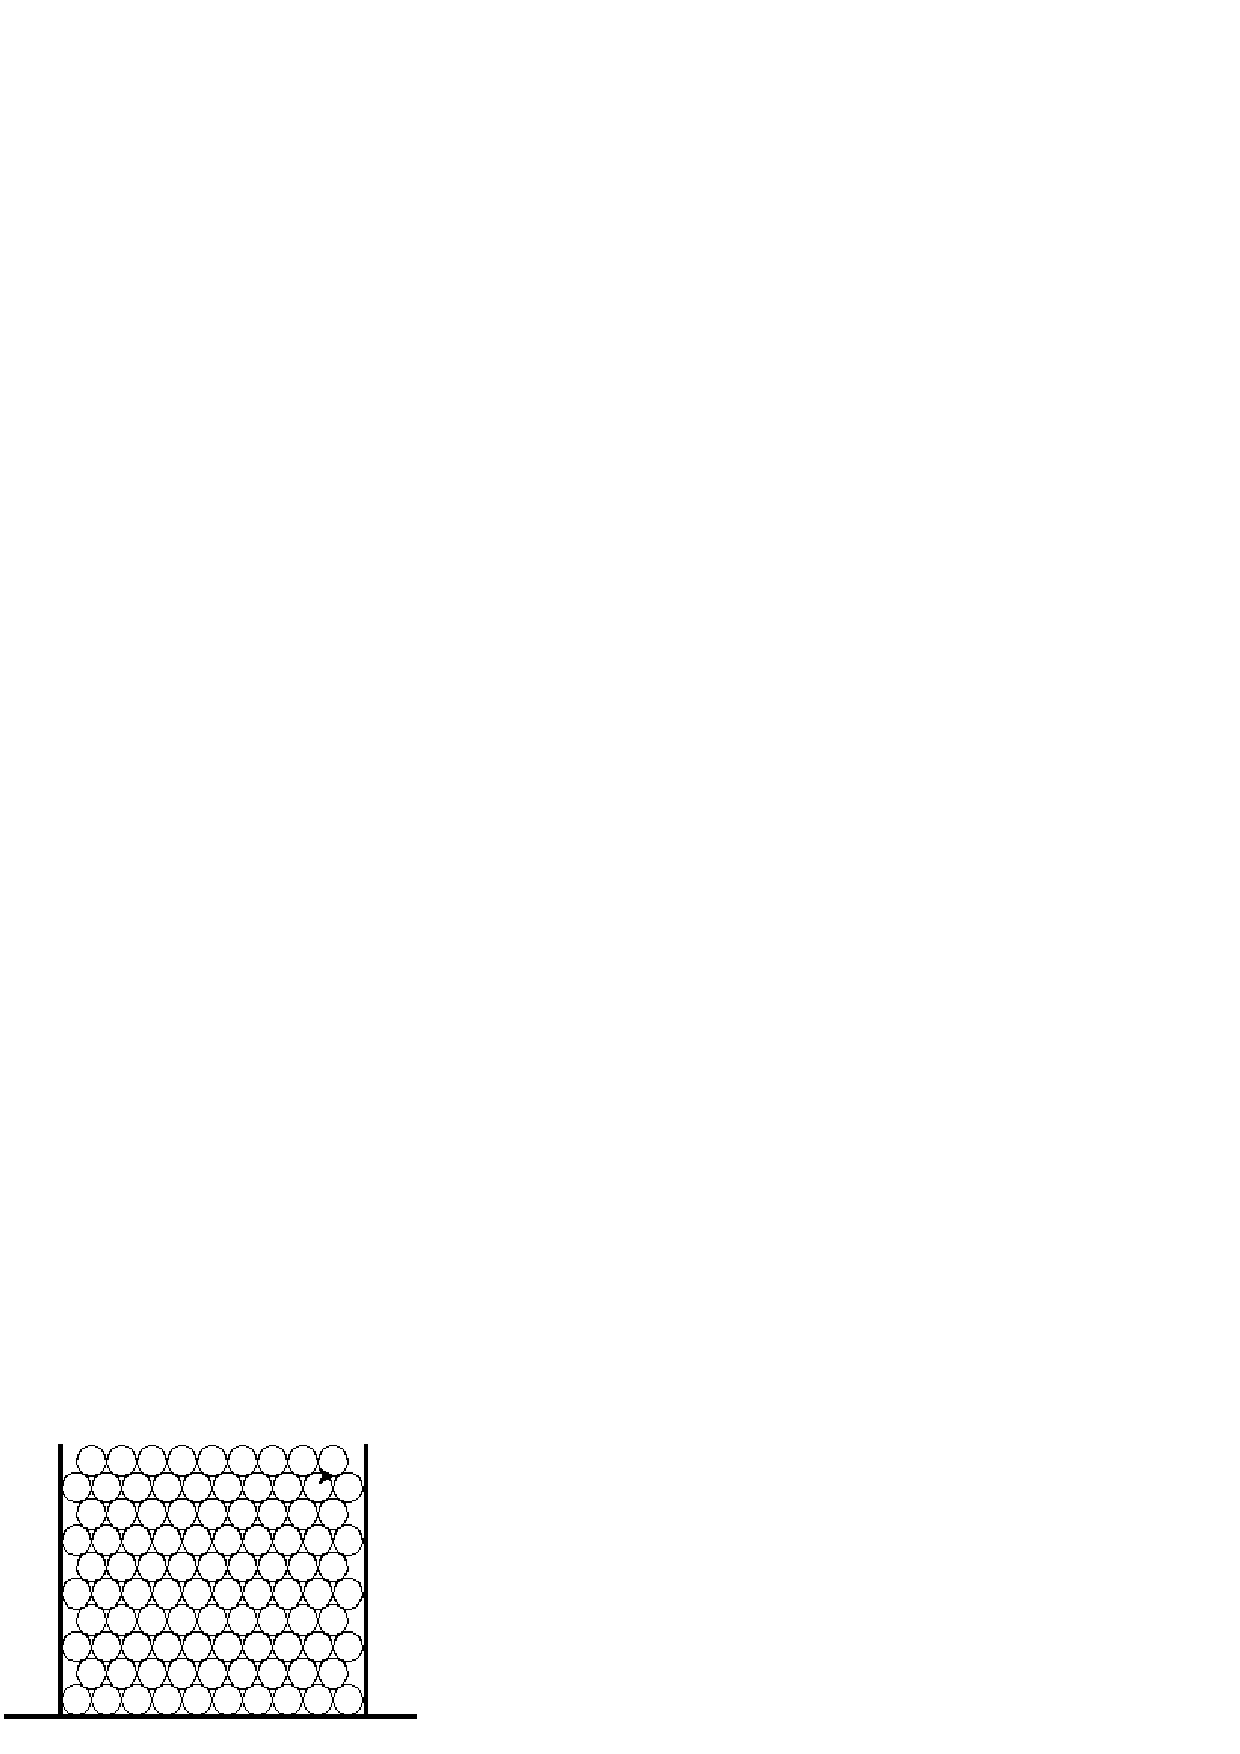
\includegraphics[width=3cm]{stere.pdf}
\end{minipage}

\paragraph{Méthode} On commence par poser sur le sol une première couche horizontale
de 10 rondins; on dispose par dessus en quinconce une deuxième rangée de 9 rondins puis
une troisième rangée de 10 rondins, et ainsi de suite jusqu'à superposer
$10$ rangées horizontales alternativement de 10 et 9 rondins.

\paragraph{Questions} 
On décompose le problème en deux sous-problèmes : empiler des rangées, aligner des rondins pour faire une rangée.

\begin{question}[«~ranger le bois~» : les rangées] Proposer un algorithme pour 
construire un stère de bois en supposant que l'on sait manipuler directement
une rangée horizontale de rondins.
\end{question}

\begin{question}[«~ranger le bois~» : une rangée] Proposer un algorithme
pour construire une rangée horizontale de rondins de bois.
\end{question}

\begin{question}[«~ranger le bois~» : le stère] Proposer un algorithme
pour construire un stère de \linebreak bois.
\end{question}


%-------------------------------------------------------------------------
\subsection{Généralisation}
%-------------------------------------------------------------------------
Une boucle permet de traiter une séquence d'éléments un par un, 
les uns après les autres (\emph{placer une rangée, puis une autre, puis une autre\ldots}), et pour chaque élément, 
on peut vouloir traiter autre chose de manière systématique (\emph{aligner les rondins}).
L'algorithme sera ainsi constitué d'une boucle principale (\emph{qui place les rangées}) et
dans le corps de cette boucle principale, on dit aussi «~à l'intérieur de la boucle~», 
une boucle secondaire (\emph{qui aligne les rondins pour faire une rangée}).
La boucle secondaire peut elle-même contenir une boucle, et ainsi de suite.


\begin{question}[boucles imbriquées : exécutions]
Qu'affichent les itérations suivantes ?

\begin{minipage}[t]{6cm}\tt
\begin{Verbatim}
for i in range(10) :
    j = 10 - i
    while j > 0 :
        print('*',end='')
        j = j - 1
    print()
\end{Verbatim}
\end{minipage}
\hfill
\begin{minipage}[t]{6cm}\tt
\begin{Verbatim}
i = 0
while i < 10 :
    for j in range(i) :
        print('*',end='')
    print()
    i = i + 1
\end{Verbatim}
\end{minipage}

\end{question}

L'approche efficace pour résoudre un problème (\emph{ranger le bois}) consiste
souvent à le décomposer en plusieurs sous-problèmes plus simples
(\emph{placer une rangée}\ldots) qui seront étudiés
séparément. Ces sous-problèmes peuvent éventuellement être eux-mêmes décomposés 
à leur tour (\emph{aligner les rondins}\ldots), et ainsi de suite.
Le concepteur de l'algorithme définit la structuration d'un problème en sous-problèmes : 
il divise le problème en sous-problèmes pour mieux le contrôler (\emph{diviser pour régner}).
Lorsque les problèmes et sous-problèmes correspondent à des boucles, on obtiendra
une structuration en boucles imbriquées et/ou en boucles successives.

\begin{question}[boucles imbriquées : imbriquées ou successives ?]
A partir de deux exemples sim\-ples et comparables, illustrer et expliquer la différence
entre deux boucles imbriquées et deux boucles successives.
Dessiner les diagrammes \uml{} correspondants.
\end{question}

%-------------------------------------------------------------------------
\subsection{Applications}
%-------------------------------------------------------------------------
\begin{question}[boucles imbriquées : tables de vérité] Ecrire un algorithme qui affiche
la table de vérité du circuit logique suivant, où $a$, $b$ et $c$ sont les entrées et 
$s_0, s_1, \ldots, s_7$ les sorties.
$$\includegraphics[width=4cm,angle=90]{decodeur.pdf}$$
\end{question}

\begin{question}[boucles imbriquées : tables de multiplication] Ecrire un algorithme
qui affiche\linebreak successivement les 10 premières tables de multiplication de deux manières 
différentes : \\
d'abord sous la forme :
\begin{minipage}[t]{3cm}\tt
\begin{Verbatim}
3 x 0 = 0
3 x 1 = 3
3 x 2 = 6
3 x 3 = 9
...
3 x 9 = 27
\end{Verbatim}
\end{minipage}
\hfill
puis sous la forme :
\begin{minipage}[t]{3cm}\tt
\begin{Verbatim}
0 x 3 = 0
1 x 3 = 3
2 x 3 = 6
3 x 3 = 9
...
9 x 3 = 27
\end{Verbatim}
\end{minipage}
\end{question}

\begin{question}[boucles imbriquées : triangle de Pascal] Ecrire un algorithme qui affiche le triangle de Pascal jusqu'à l'ordre $n$. 
Chaque ligne $i$ de ce triangle est composée des coefficients $c_{ij}$ du binôme 
$\displaystyle (x + y)^i = \sum_{j=0}^{i} c_{ij}x^{i-j}y^j = \sum_{j=0}^{i} \frac{i!}{j!(i-j)!}x^{i-j}y^j$ où $\forall i,$ $c_{i0} = c_{ii} = 1$ et $c_{ij} = c_{i-1,j} + c_{i-1,j-1}$ $\forall j,\ 0 < j < i$.

\noindent
Les 8 premières lignes du triangle de Pascal sont donc les suivantes :
\hfill\begin{minipage}[t]{4cm}\tt
\begin{Verbatim}
1
1 1
1 2 1
1 3 3 1
1 4 6 4 1
1 5 10 10 5 1
1 6 15 20 15 6 1
1 7 21 35 35 21 7 1
\end{Verbatim}
\end{minipage}	
\end{question}

%\begin{question}[boucles imbriquées : produits de matrices] Ecrire un algorithme qui calcule
%le produit $C$ de 2 matrices $A$ et $B$ respectivement de dimensions $(n,r)$ et $(r,m)$.
%
%$$\begin{minipage}{5cm}
%\includegraphics[width=4cm]{produit-matrices.pdf}
%\end{minipage}
%\hspace*{1cm}
%c_{ij} = \sum_{k=0}^{r-1}a_{ik}\cdot b_{kj}$$
%
%\end{question}


%-------------------------------------------------------------------------
%\newpage
\subsection{Entraînement}
%-------------------------------------------------------------------------

%-------------------------------------------------------------------------
\subsubsection{Enoncé}
%-------------------------------------------------------------------------

\paragraph{Objectif :} en utilisant les instructions de la tortue \logo{}
(module \texttt{turtle}), écrire un algorithme qui dessine un motif géométrique
régulier composé de polygones réguliers.


\paragraph{Méthode :} 
construire l'algorithme en décomposant le problème en 3 niveaux :
\begin{enumerate}
\item le tracé du polygone élémentaire,
\item le tracé d'une ligne de polygones élémentaires,
\item le tracé du motif de lignes de polygones élémentaires.
\end{enumerate}
On pourra commencer soit par l'étape de plus haut niveau (le motif), 
soit par l'étape de plus bas niveau (le polygone élémentaire).

\paragraph{Vérification :} vérifier l'algorithme sous \python{} en comparant 
le tracé obtenu avec la figure de l'énoncé.

%-------------------------------------------------------------------------
\subsubsection{Exemple}
%-------------------------------------------------------------------------
On considère le motif composé de ($5\times 4$)
hexagones réguliers de côté de longueur $d$ représenté ci-dessous :

$$\begin{minipage}{6.75cm}
\begin{tikzpicture}[scale=0.5]\footnotesize
\draw[color=lightgray](-6,-4) grid[xstep=1,ystep=1] (6,4);
%\foreach \x in {-6,-5,...,6} \draw(\x,-4) node[below]{\x};
%\foreach \y in {-4,-3,...,4} \draw(-6,\y) node[left]{\y};
%\filldraw(0,0) circle (0.1);
%\draw[->] (-6,0) -- (6,0);
%\draw (6,0) node[right]{$x$} ;
%\draw[->] (0,-4) -- (0,4);
%\draw (0,4) node[above]{$y$};
\foreach \y in {-4,-2.27,-0.53,1.20} \foreach \x in {-5,-3,-1,1,3} \hexagone{\x}{\y} ;
\draw(5,{-4+3*sqrt(3)/2}) node[right]{$d\sqrt{3}$};
\draw (-6,{-4+sqrt(3)}) -- (6,{-4+sqrt(3)});
\draw (-6,{-4+2*sqrt(3)}) -- (6,{-4+2*sqrt(3)});
\draw[<->] (5,{-4+2*sqrt(3)}) -- (5,{-4+sqrt(3)});
\draw(0,3.5) node[above]{$2d$};
\draw[<->] (-1,3.5) -- (1,3.5);
\filldraw(-5,-4) circle (0.1);
\draw(-5,-4) node[below]{$(x_0,y_0)$};
\end{tikzpicture}
\end{minipage}$$


\paragraph{Méthode}
On écrit successivement le code qui trace un motif de $m$ lignes d'hexagones,
une ligne de $n$ hexagones et un hexagone, en supposant à chaque étape que le niveau inférieur
est réalisé  :
\begin{enumerate}
\item Tracé d'un motif de $m$ lignes d'hexagones\\
	Pour chaque ligne d'indice $j$,
	on positionne le crayon en bas à gauche de la ligne :
	les lignes étant alignées verticalement, l'abscisse $x$ ne change pas,
	l'ordonnée $y$ doit par contre être déplacée 
	vers le haut de $d\sqrt{3}$ à chaque changement d'indice.
	Une fois positionnée, on trace la ligne d'hexagones.

\begin{Verbatim}	
# dessin d'un motif de m lignes d'hexagones
for j in range(m) :
    x, y = x0, y0 + j*d*sqrt(3)
    # dessin d'une ligne de n hexagones
\end{Verbatim}

\item Tracé d'une ligne de $n$ hexagones\\
	Pour chaque hexagone d'indice $i$, on positionne le crayon en bas à gauche de 
	l'hexagone : les hexagones d'une même ligne étant alignés horizontalement,
	l'ordonnée $y$ ne change pas, l'abscisse $x$ doit par contre être déplacée
	vers la gauche de $2d$ à chaque changement d'indice.
	Une fois positionné, on trace l'hexagone.
\begin{Verbatim}	
# dessin d'une ligne de n hexagones
for i in range(n) :
    x = x0 + 2*i*d
    # dessin d'un hexagone
\end{Verbatim}

\item Tracé d'un hexagone\\
	Les motifs considérés ici sont composés de polygones réguliers;
	en utilisant les instructions de la tortue \logo, l'algorithme suivant permet 
	de dessiner un polygone régulier de $c$ côtés de longueur $d$.
$$\begin{minipage}{6cm}
\begin{Verbatim}
for k in range(c) :
    forward(d)
    left(360/c)
\end{Verbatim}
\end{minipage}
\begin{tabular}{l@{ : }l}
$c$ & polygone 	\\
\hline
3 	& triangle 	\\
4 	& carré 	\\
5 	& pentagone	\\
6	& hexagone 	\\
7   & heptagone \\
8	& octogone  \\
9   & ennéagone \\
\multicolumn{2}{l}{\ldots }
\end{tabular}$$
$$\includegraphics[width=0.8\textwidth]{pave.png}$$

On se déplace donc, crayon levé, jusqu'à l'origine en bas à gauche d'un hexagone,
puis on trace l'hexagone ($c = 6$).
\begin{Verbatim}	
# dessin d'un hexagone
up()
goto(x,y)
down()
for k in range(c) :
    forward(d)
    left(360/c)
\end{Verbatim}

\end{enumerate}

\noindent
\begin{minipage}[t]{7cm}
\paragraph{Résultat} En \python, l'algorithme correspondant, présenté ci-contre, 
est donc composé de 3 boucles imbriquées. 
Il faut inclure le module \texttt{math} pour utiliser la fonction \texttt{sqrt()}
ainsi que le module \texttt{turtle} pour les fonctions de manipulation de la tortue \logo{}
(\texttt{up()}, \texttt{down()}, \texttt{goto()}, \texttt{left()} et \texttt{forward()}).
Pour le tester, on fixera les valeurs de $c$ (nombre de côtés, 6 pour un hexagone),
$d$ (longueur du côté de l'hexagone), $n$ (nombre d'hexagones dans une ligne) et $m$ 
(nombre de lignes) ainsi que l'origine du motif  $(x_0,y_0)$.
Pour le vérifier, on comparera le tracé obtenu avec celui de la figure du motif
présentée plus haut en début de section.
\end{minipage}
\hfill
\begin{minipage}[t]{8.25cm}\footnotesize
\begin{lstlisting}
from math import *
from turtle import *
# initialisation du motif
c, d = 6, 20
n, m = 5, 4
x0, y0 = 0, 0
# dessin du motif
for j in range(m) :
    x, y = x0, y0 + j*d*sqrt(3)
    # dessin d'une ligne d'hexagones
    for i in range(n) :
        x = x0 + 2*i*d
        # dessin d'un hexagone
        up()
        goto(x,y)
        down()
        for k in range(c) :
            forward(d)
            left(360/c)
\end{lstlisting}
\end{minipage}

\paragraph{Vérifications} 
on compare le tracé obtenu lors de l'exécution de l'algorithme précédent avec la figure donnée
en début de section.
\vspace*{3mm}

\noindent\begin{minipage}{6.75cm}
\centerline{\fbox{\begin{tikzpicture}[scale=0.5]\footnotesize
\draw[color=lightgray](-6,-4) grid[xstep=1,ystep=1] (6,4);
%\foreach \x in {-6,-5,...,6} \draw(\x,-4) node[below]{\x};
%\foreach \y in {-4,-3,...,4} \draw(-6,\y) node[left]{\y};
%\filldraw(0,0) circle (0.1);
%\draw[->] (-6,0) -- (6,0);
%\draw (6,0) node[right]{$x$} ;
%\draw[->] (0,-4) -- (0,4);
%\draw (0,4) node[above]{$y$};
\foreach \y in {-4,-2.27,-0.53,1.20} \foreach \x in {-5,-3,-1,1,3} \hexagone{\x}{\y} ;
\draw(5,{-4+3*sqrt(3)/2}) node[right]{$d\sqrt{3}$};
\draw (-6,{-4+sqrt(3)}) -- (6,{-4+sqrt(3)});
\draw (-6,{-4+2*sqrt(3)}) -- (6,{-4+2*sqrt(3)});
\draw[<->] (5,{-4+2*sqrt(3)}) -- (5,{-4+sqrt(3)});
\draw(0,3.5) node[above]{$2d$};
\draw[<->] (-1,3.5) -- (1,3.5);
\filldraw(-5,-4) circle (0.1);
\draw(-5,-4) node[below]{$(x_0,y_0)$};
\end{tikzpicture}}}
\centerline{figure de l'énoncé}
\end{minipage}
\hfill
\begin{minipage}{6.25cm}
\centerline{\fbox{\includegraphics[width=6cm]{pavage.png}}}
\centerline{tracé \python}
\end{minipage}
\vspace*{3mm}

\noindent Les figures sont bien similaires.
%-------------------------------------------------------------------------
\subsubsection{Questions}
%-------------------------------------------------------------------------
En utilisant les instructions de la tortue \logo{}
(module \texttt{turtle}), écrire un algorithme qui dessine un motif géométrique
composé de $(n\times m)$ pavés élémentaires disposés régulièrement sur une grille
ou disposés en quinconce sur la grille.
\vspace*{3mm}

\centerline{\includegraphics[width=4cm]{grille-1.pdf}\hspace*{1cm}\includegraphics[width=4cm]{grille-2.pdf}}
\centerline{\makebox[4cm]{alignés}\hspace*{1cm}\makebox[4cm]{en quinconce}}

\begin{minipage}[t]{7cm}
\begin{enumerate}
\item \begin{minipage}{1.75cm}\includegraphics[height=1cm]{etoile-1.pdf}\end{minipage} alignés
\item \begin{minipage}{1.75cm}\includegraphics[height=1cm]{etoile-1.pdf}\end{minipage} en quinconce
\item \begin{minipage}{1.75cm}\includegraphics[height=1cm]{cercle-1.pdf}\end{minipage} alignés
\item \begin{minipage}{1.75cm}\includegraphics[height=1cm]{cercle-1.pdf}\end{minipage} en quinconce
\item \begin{minipage}{1.75cm}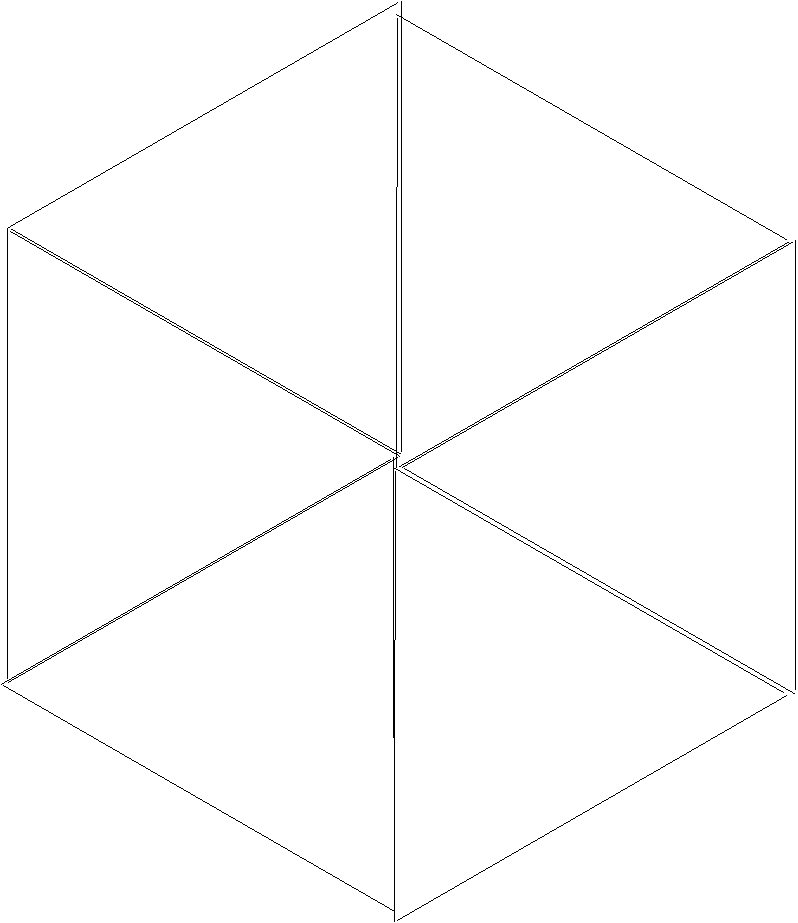
\includegraphics[height=1cm]{hexagone-1.pdf}\end{minipage} alignés
\item \begin{minipage}{1.75cm}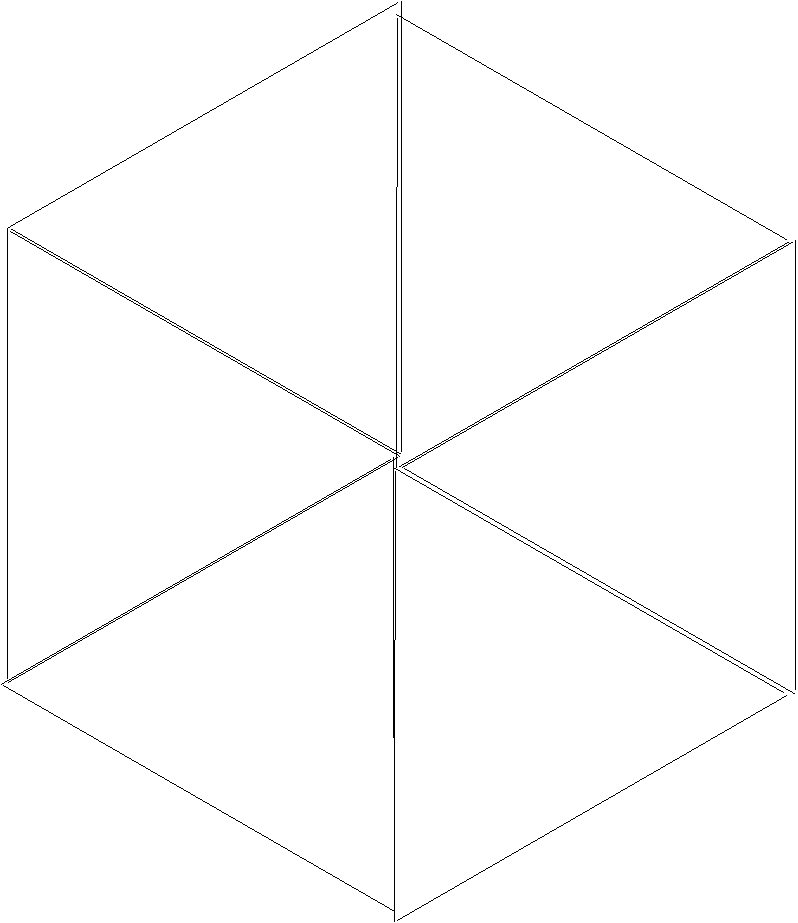
\includegraphics[height=1cm]{hexagone-1.pdf}\end{minipage} en quinconce
\item \begin{minipage}{1.75cm}
\includegraphics[height=1cm]{triangle-1.pdf}\end{minipage} alignés
\item \begin{minipage}{1.75cm}
\includegraphics[height=1cm]{triangle-1.pdf}\end{minipage} en quinconce
\item \begin{minipage}{1.75cm}\includegraphics[height=1cm]{losange-1.pdf}\end{minipage} alignés
\item \begin{minipage}{1.75cm}\includegraphics[height=1cm]{losange-1.pdf}\end{minipage} en quinconce
\item \begin{minipage}{1.75cm}\includegraphics[height=1cm]{carre-1.pdf}\end{minipage} alignés
\item \begin{minipage}{1.75cm}\includegraphics[height=1cm]{carre-1.pdf}\end{minipage} en quinconce
\end{enumerate}
\end{minipage}
\hfill
\begin{minipage}[t]{7cm}
\begin{enumerate}\setcounter{enumi}{12}
\item \begin{minipage}{1.75cm}\includegraphics[height=1cm]{etoile-2.pdf}\end{minipage} alignés
\item \begin{minipage}{1.75cm}\includegraphics[height=1cm]{etoile-2.pdf}\end{minipage} en quinconce
\item \begin{minipage}{1.75cm}\includegraphics[height=1cm]{cercle-2.pdf}\end{minipage} alignés
\item \begin{minipage}{1.75cm}\includegraphics[height=1cm]{cercle-2.pdf}\end{minipage} en quinconce
\item \begin{minipage}{1.75cm}\includegraphics[height=1cm]{hexagone-2.pdf}\end{minipage} alignés
\item \begin{minipage}{1.75cm}\includegraphics[height=1cm]{hexagone-2.pdf}\end{minipage} en quinconce
\item \begin{minipage}{1.75cm}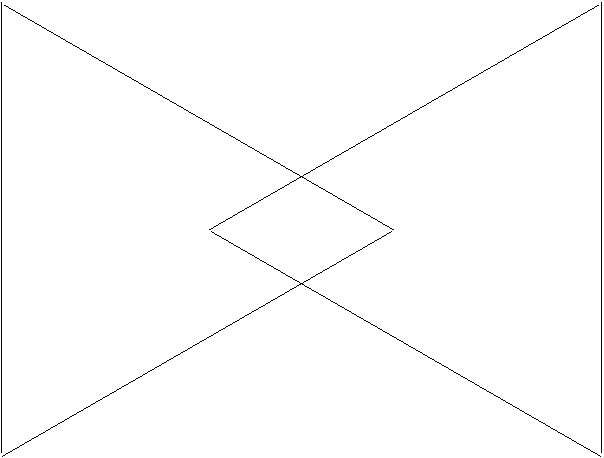
\includegraphics[height=1cm]{triangle-2.pdf}\end{minipage} alignés
\item \begin{minipage}{1.75cm}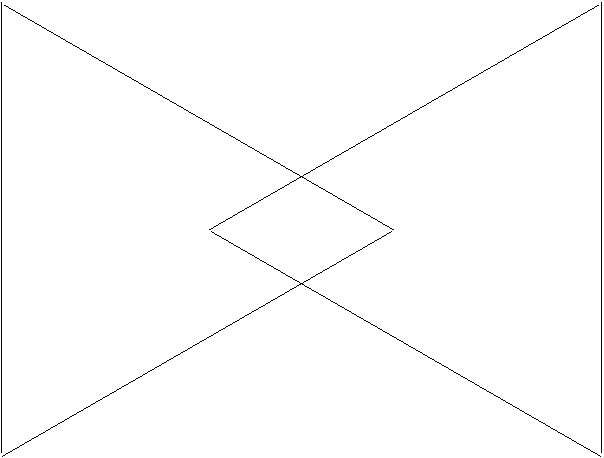
\includegraphics[height=1cm]{triangle-2.pdf}\end{minipage} en quinconce
\item \begin{minipage}{1.75cm}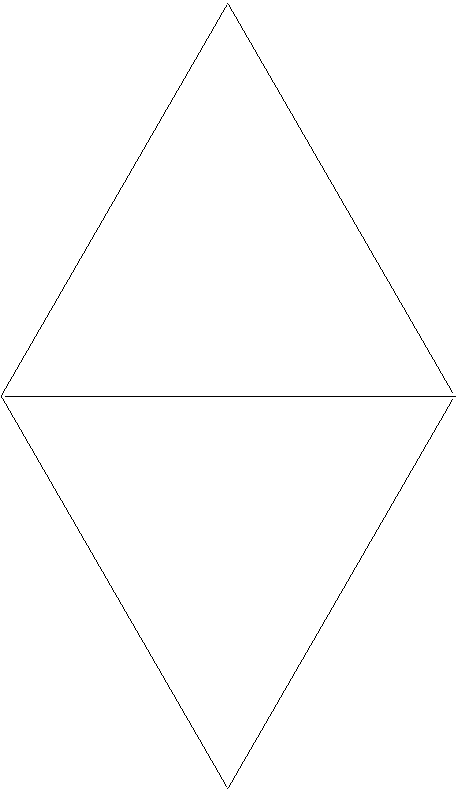
\includegraphics[height=1cm]{losange-2.pdf}\end{minipage} alignés
\item \begin{minipage}{1.75cm}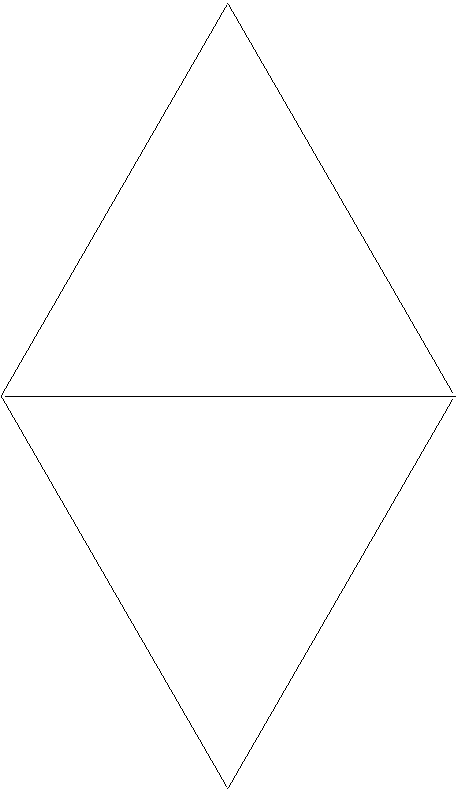
\includegraphics[height=1cm]{losange-2.pdf}\end{minipage} en quinconce
\item \begin{minipage}{1.75cm}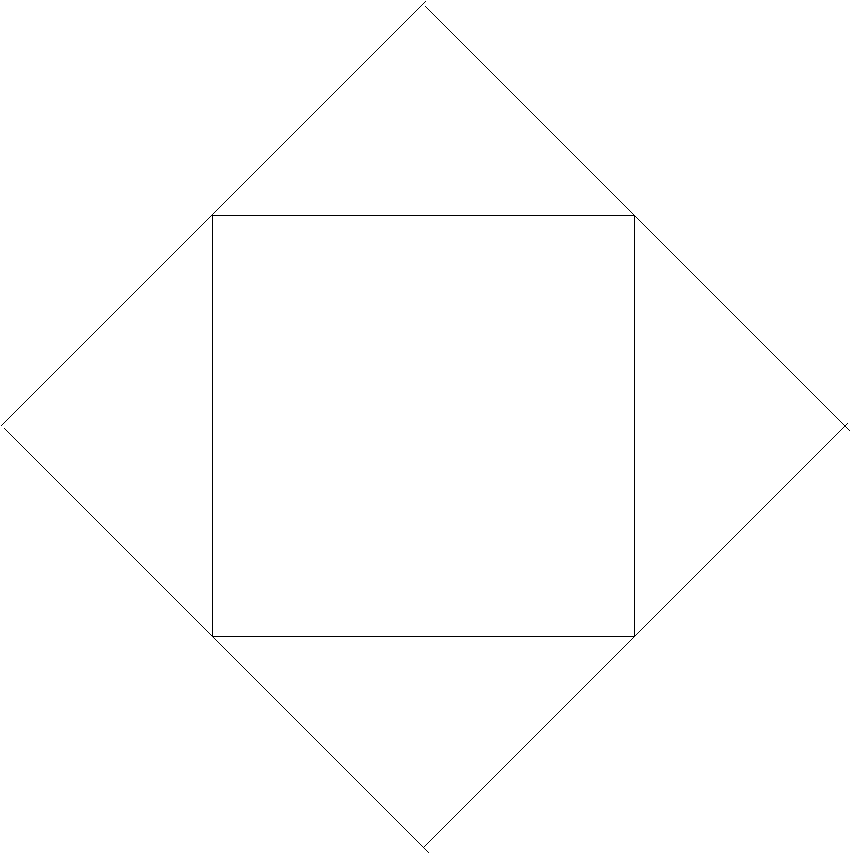
\includegraphics[height=1cm]{carre-2.pdf}\end{minipage} alignés
\item \begin{minipage}{1.75cm}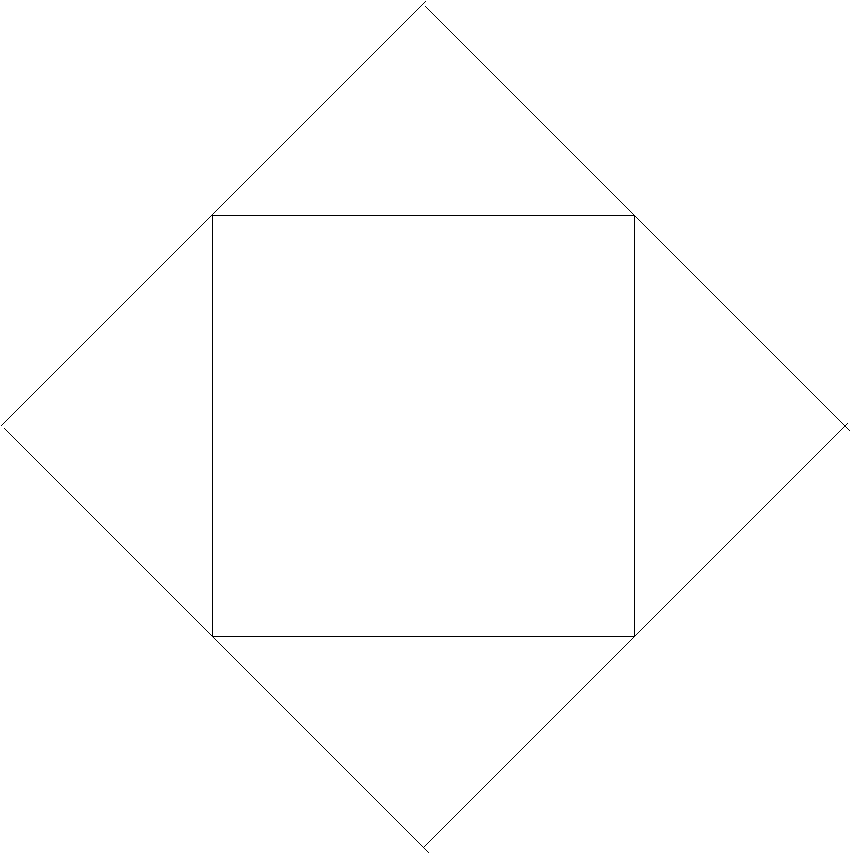
\includegraphics[height=1cm]{carre-2.pdf}\end{minipage} en quinconce
\end{enumerate}
\end{minipage}

%-------------------------------------------------------------------------
\subsection{Révisions}
%-------------------------------------------------------------------------

$$\begin{tabular}{|ll@{ : }l|}
\hline
\textbf{Cours} & \cite{cours} & chapitre 2, sections 2.4.2 à 2.4.4 \\
\textbf{TD}    & \cite{td}    & exercices 2.20 à 2.24 et 2.34 \\
\hline
\end{tabular}$$


%-------------------------------------------------------------------------
\newpage
%\setcounter{section}{8}
\section{Comment spécifier une fonction ?}\label{sec:specification}
%-------------------------------------------------------------------------
	\input{q-info-S1-specification.tex}

%-------------------------------------------------------------------------
\newpage
%\setcounter{section}{9}
\section{Qu'est-ce que la récursivité ?}\label{sec:recursivite}
%-------------------------------------------------------------------------
	\input{q-info-S1-recursivite.tex}

%-------------------------------------------------------------------------
\newpage
%\setcounter{section}{10}
\section{Comment trier une séquence ?}\label{sec:sequences}
%-------------------------------------------------------------------------
	\input{q-info-S1-sequences.tex}

%-------------------------------------------------------------------------
\newpage
%\setcounter{section}{11}
\section{Tout en un ?}\label{sec:conclusion}
%-------------------------------------------------------------------------
	%-------------------------------------------------------------------------
% q-info-S1-conclusion.tex
%-------------------------------------------------------------------------
\def\reseau{%
\begin{picture}(8.5,4.5)        
\put(1,2.5){\makebox(0,0){$\bullet$}}
\put(0.7,2.5){\makebox(0,0){ s}} 
\put(1.75,3){\makebox(0,0){\tiny 3}}  % s-a 
\put(1.75,2){\makebox(0,0){\tiny 4}} % s-d
\put(2.75,2.5){\makebox(0,0){\tiny 5}}  % a-d 
\put(3.5,3.75){\makebox(0,0){\tiny 4}}  % a-b
\put(4.75,2.5){\makebox(0,0){\tiny 5}}  % b-e
\put(3.5,1.25){\makebox(0,0){\tiny 2}}  % d-e
\put(5.5,1.25){\makebox(0,0){\tiny 4}}  % e-f
\put(7.25,2){\makebox(0,0){\tiny 3}}  % f-g
\put(5.5,3.75){\makebox(0,0){\tiny 4}}  % b-c
\put(1,2.5){\line(1,1){1.5}}
\put(1,2.5){\line(1,-1){1.5}}
\put(2.5,4){\makebox(0,0){$\bullet$}}
\put(2.5,4.3){\makebox(0,0){ a}}
\put(2.5,1){\makebox(0,0){$\bullet$}}
\put(2.5,0.75){\makebox(0,0){ d}} 
\put(2.5,4){\line(1,0){4}}
\put(2.5,1){\line(1,0){4}}
\put(4.5,1){\makebox(0,0){$\bullet$}} 
\put(4.5,0.75){\makebox(0,0){ e}}
\put(6.5,1){\makebox(0,0){$\bullet$}} 
\put(6.5,0.75){\makebox(0,0){ f}}
\put(6.5,1){\line(1,1){1.5}}
\put(8,2.5){\makebox(0,0){$\bullet$}} 
\put(8.2,2.5){\makebox(0,0){ g}} 
\put(4.5,4){\makebox(0,0){$\bullet$}} 
\put(4.5,4.3){\makebox(0,0){ b}}
\put(6.5,4){\makebox(0,0){$\bullet$}}
\put(6.5,4.3){\makebox(0,0){ c}} 
\put(2.5,4){\line(0,-1){3}} 
\put(4.5,4){\line(0,-1){3}}
%\put(4.5,0){\makebox(0,0){\normalsize r\'eseau routier}} 
\end{picture}}

\noindent\begin{minipage}{10cm}
\begin{description}
\item[Objectif :] mettre en \oe uvre l'ensemble des notions abordées dans ce document
	à travers l'exemple général de la recherche d'un chemin dans un graphe.
\end{description}
\end{minipage}
\hfill
\begin{minipage}{4cm}
Graphe\\
\fbox{\begin{tikzpicture}[scale=1]\scriptsize
\node[draw,circle] (A) at (0,0) {\texttt{n1}};
\node[draw,circle] (B) at (0,1) {\texttt{n2}};
\node[draw,circle] (C) at (1,0) {\texttt{n3}};
\node[draw,circle] (D) at (2,1) {\texttt{n4}};
\node[draw,circle] (E) at (3,1) {\texttt{n5}};
\draw (A) -- (B);
\draw (0,0.5) node[left] {4};
\draw (B) -- (C);
\draw (0.5,0.5) node[right] {3};
\draw (A) to[out=-90,in=-90] (D);
\draw (B) to[out=60,in=120] (D);
\draw (B) -- (D);
\draw (C) -- (D);
\draw (1.5,0.5) node[left] {2};
\draw (1,1) node[above] {5};
\draw (1.5,-0.4) node[below] {6};
\draw (1,1.75) node[above] {6};
\draw (D) -- (E);
\draw (2.5,1) node[above] {1};
\draw (B) to[out=90,in=90] (E);
\draw (1.5,2.25) node[above] {2};
\coordinate[shift={(0mm,-1cm)}] (n) at (E.south);
\draw[rounded corners=30pt] (E.south west) -- (n) -- (E.south east);
\draw (3,0) node {3};
\end{tikzpicture}}
\end{minipage}

%-------------------------------------------------------------------------
\subsection{Exemple}
%-------------------------------------------------------------------------

\paragraph{Enoncé :}
Dans le premier exemple introductif (section \ref{sec:algo}, exemple \ref{ex:restaurant} 
page \pageref{ex:restaurant} : «~aller au restaurant~»)
un touriste devait rejoindre un restaurant depuis son hôtel.
On peut, en première approximation, assimiler le plan de la ville à un graphe dont 
les n\oe uds ($\bullet$) sont les carrefours et les arcs ($\rule[0.5ex]{1cm}{1pt}$)
les tronçons de rues entre deux carrefours, comme suggéré sur la figure ci-dessous. 
Le problème ainsi transposé devient la recherche d'un chemin d'un carrefour à un autre
au sein d'un réseau urbain connu sans passer deux fois par le même carrefour.
\vspace*{3mm}

%C'est ce problème plus abstrait qui est traité dans cette section car il met en \oe uvre l'ensemble des notions abordées précédemment. Une fois résolu, nous pourrons l'appliquer
%à la recherche d'un chemin dans un réseau routier et l'étendre à titre d'exemples à 
%des applications «~ludiques~».

\noindent\begin{minipage}{7cm}
\includegraphics[width=7cm]{plan.pdf}
\end{minipage}
\hfill
\begin{minipage}{7cm}
\begin{tikzpicture}[scale=1]\scriptsize
\draw (0,0) -- (4,0) node[midway,below] {rue Jean Jaurès};
\draw (0,1) -- (4,1) node[midway,below] {rue Duret};
\draw (0,2) -- (4,2) node[midway,below] {rue Massillon};
\draw (0,3) -- (4,3) node[midway,above] {rue Charles Berthelot};
\draw (0,0) -- (0,3) node[midway,above,rotate=90] {rue Danton};
\draw (1,0) -- (1,3);
\draw (2,0) -- (2,3);
\draw (3,0) -- (3,3);
\draw (4,0) -- (4,3) node[midway,below,rotate=90] {rue Kerfautras};
\foreach \x in {0,1,...,4} \foreach \y in {0,1,2,3} \draw (\x,\y) node {$\bullet$};
\draw[color=red,thick] (0,2) circle(0.3);
\draw[color=red,->] (0.5,2.5) node[right] {restaurant} -- (0.225,2.225);
\draw[color=red,thick] (4,0) circle(0.3);
\draw[color=red,->] (4.75,0) node[right] {hôtel} -- (4.3,0);
\end{tikzpicture}
\end{minipage}
\vspace*{3mm}

\paragraph{Méthode :} Rechercher un chemin entre deux n\oe uds d'un graphe sans passer 
deux fois par le même n\oe ud revient à parcourir un arbre de recherche comme le montre 
la figure ci-dessous. Dans le réseau routier (à gauche de la figure), on cherche à se rendre de 
\texttt{s} à \texttt{g}, ce qui revient à parcourir l'arbre de recherche (à droite de la figure)
dans lequel on observe qu'il y a 4 chemins différents pour se rendre de \texttt{s} à \texttt{g} :
\texttt{[s,a,b,e,f,g]} de 19 km, \texttt{[s,a,d,e,f,g]} (17 km), \texttt{[s,d,a,b,e,f,g]} (25 km)
et \texttt{[s,d,e,f,g]} (13 km), les autres chemins étant des impasses dans ce contexte. 
\vspace*{3mm}

\noindent\begin{minipage}{5.25cm}
\setlength\unitlength{0.6cm}\footnotesize
\reseau
\end{minipage}
\hfill$\longrightarrow$\hfill
\begin{minipage}{8.75cm}
\setlength{\unitlength}{0.6cm}\footnotesize
\begin{picture}(14,6)%\color{lightgray}
%\put(7,7){\makebox(0,1){\LARGE Pour aller de {s} \`a {g}}} 
\put(7,6){\makebox(0,0){$\bullet$}}
\put(7,6.3){\makebox(0,0){s}}
\put(7,6){\line(-4,-1){4}}
\put(7,6){\line(4,-1){4}} 
\put(3,5.3){\makebox(0,0){a}}
\put(3,5){\makebox(0,0){$\bullet$}}
\put(11,5.3){\makebox(0,0){d}}
\put(11,5){\makebox(0,0){$\bullet$}}
\put(3,5){\line(-2,-1){2}}
\put(3,5){\line(2,-1){2}}
\put(1,4.3){\makebox(0,0){b}}
\put(1,4){\makebox(0,0){$\bullet$}}
\put(5,4.3){\makebox(0,0){d}}
\put(5,4){\makebox(0,0){$\bullet$}}
\put(1,4){\line(-1,-1){1}}
\put(1,4){\line(1,-1){1}}   
\put(0,2.7){\makebox(0,0){c}}
\put(0,3){\makebox(0,0){$\bullet$}}
\put(2,3.3){\makebox(0,0){e}}
\put(2,3){\makebox(0,0){$\bullet$}}
\put(2,3){\line(-1,-1){1}}
\put(2,3){\line(1,-1){1}}    
\put(1,1.7){\makebox(0,0){d}}
\put(1,2){\makebox(0,0){$\bullet$}}
\put(3,2.3){\makebox(0,0){f}}
\put(3,2){\makebox(0,0){$\bullet$}}
\put(3,2){\line(0,-1){1}}
\put(3,0.7){\makebox(0,0){g}} 
\put(3,1){\makebox(0,0){$\bullet$}}
\put(5,4){\line(0,-1){1}}
\put(5.3,3.1){\makebox(0,0){e}}
\put(5,3){\makebox(0,0){$\bullet$}}
\put(5,3){\line(-1,-1){1}}
\put(5,3){\line(1,-1){1}}   
\put(4,2.3){\makebox(0,0){b}}
\put(4,2){\makebox(0,0){$\bullet$}}
\put(6,2.3){\makebox(0,0){f}}
\put(6,2){\makebox(0,0){$\bullet$}}
\put(4,2){\line(0,-1){1}}
\put(4,0.7){\makebox(0,0){c}}
\put(4,1){\makebox(0,0){$\bullet$}}
\put(6,2){\line(0,-1){1}}
\put(6,0.7){\makebox(0,0){g}}
\put(6,1){\makebox(0,0){$\bullet$}}
\put(11,5){\line(-2,-1){2}}
\put(9,4.3){\makebox(0,0){a}}
\put(9,4){\makebox(0,0){$\bullet$}}
\put(9,4){\line(0,-1){1}}
\put(9.3,3.1){\makebox(0,0){b}}
\put(9,3){\makebox(0,0){$\bullet$}}
\put(9,3){\line(-1,-1){1}}
\put(9,3){\line(1,-1){1}}   
\put(8,1.7){\makebox(0,0){c}}
\put(8,2){\makebox(0,0){$\bullet$}}
\put(10,2.3){\makebox(0,0){e}}
\put(10,2){\makebox(0,0){$\bullet$}}
\put(10,2){\line(0,-1){1}}
\put(10.3,1){\makebox(0,0){f}}
\put(10,1){\makebox(0,0){$\bullet$}}
\put(10,1){\line(0,-1){1}}
\put(10,-0.3){\makebox(0,0){g}} 
\put(10,0){\makebox(0,0){$\bullet$}} 
\put(11,5){\line(2,-1){2}}
\put(13,4.3){\makebox(0,0){e}}
\put(13,4){\makebox(0,0){$\bullet$}}
\put(13,4){\line(-1,-1){1}}
\put(13,4){\line(1,-1){1}}   
\put(12,3.3){\makebox(0,0){b}}
\put(12,3){\makebox(0,0){$\bullet$}}
\put(12,3){\line(-1,-1){1}}
\put(12,3){\line(1,-1){1}}   
\put(14,3.3){\makebox(0,0){f}}
\put(14,3){\makebox(0,0){$\bullet$}}
\put(14,3){\line(0,-1){1}}
\put(11,1.7){\makebox(0,0){a}}
\put(11,2){\makebox(0,0){$\bullet$}}
\put(13,1.7){\makebox(0,0){c}}  
\put(13,2){\makebox(0,0){$\bullet$}}
\put(14,1.7){\makebox(0,0){g}}
\put(14,2){\makebox(0,0){$\bullet$}}
%\color{orange}
%\thicklines
\put(7,6){\line(-4,-1){4}}
\put(3,5){\line(-2,-1){2}}
\put(1,4){\line(1,-1){1}}
\put(2,3){\line(1,-1){1}}
\put(3,2){\line(0,-1){1}}
\put(3,0){\makebox(0,0){(19)}}
\put(3,5){\line(2,-1){2}}
\put(5,4){\line(0,-1){1}}
\put(5,3){\line(1,-1){1}}
\put(6,2){\line(0,-1){1}}
\put(6,0){\makebox(0,0){(17)}}
\put(7,6){\line(4,-1){4}} 
\put(11,5){\line(-2,-1){2}}
\put(9,4){\line(0,-1){1}}
\put(9,3){\line(1,-1){1}}   
\put(10,2){\line(0,-1){1}}
\put(10,1){\line(0,-1){1}}
\put(10,-1){\makebox(0,0){(25)}}
\put(11,5){\line(2,-1){2}}
\put(13,4){\line(1,-1){1}}   
\put(14,3){\line(0,-1){1}}
\put(14,1){\makebox(0,0){(13)}}
\end{picture}
\end{minipage}
\newpage

On utilisera donc des méthodes de parcours d'arbre pour ce type de recherche
(recherche en profondeur, en largeur ou du meilleur chemin).
Dans un premier temps, nous introduirons un certain nombre de notions 
(piles, files, graphes) qui seront utiles à la recherche d'un chemin 
dans un graphe.

%-------------------------------------------------------------------------
\subsubsection{Piles et files}\label{subsec:pile}
%-------------------------------------------------------------------------

\noindent\begin{minipage}[t]{7.7cm}
{Pile : structure \textsc{Lifo}}\\
\fbox{\begin{tikzpicture}[scale=1]\scriptsize
\draw (0,0) -- (3,0);
\draw (0,1) -- (3,1);
\draw[dashed] (3,0) -- (4,0);
\draw[dashed] (3,1) -- (4,1);
\draw (4,0) -- (5,0);
\draw (4,1) -- (5,1);
\draw[dotted] (5,0) -- (6,0);
\draw[dotted] (5,1) -- (6,1);
\draw (0,0) -- (0,1);
\draw (0.5,0.5) node {\texttt{t[0]}};
\draw (1,0) -- (1,1);
\draw (1.5,0.5) node {\texttt{t[1]}};
\draw (2,0) -- (2,1);
\draw (2.5,0.5) node {\texttt{t[2]}};
\draw (3,0) -- (3,1);
\draw (4,0) -- (4,1);
\draw (5,0) -- (5,1);
\draw (4.5,0.5) node {\texttt{t[n-1]}};
\draw (4.5,1.5) node[above] {\texttt{sommet}};
\draw[->] (4.5,1.5) -- (4.5,1);
\draw (5.75,0.75) node[right] {\texttt{empiler}};
\draw (5.75,0.25) node[right] {\texttt{dépiler}};
\draw[->] (5.75,0.75) -- (5,0.75);
\draw[->] (5,0.25) -- (5.75,0.25);
\draw (2.5,0) node[below] {$\underbrace{\makebox[5cm]{}}_{\mbox{liste de \texttt{n} éléments}}$};
\end{tikzpicture}}
\end{minipage}
\hfill
\begin{minipage}[t]{8cm}
{File : structure \textsc{Fifo}}\\
\fbox{\begin{tikzpicture}[scale=1]\scriptsize
\draw[dotted] (0,0) -- (1,0);
\draw[dotted] (0,1) -- (1,1);
\draw (1,0) -- (3,0);
\draw (1,1) -- (3,1);
\draw[dashed] (3,0) -- (4,0);
\draw[dashed] (3,1) -- (4,1);
\draw (4,0) -- (5,0);
\draw (4,1) -- (5,1);
\draw[dotted] (5,0) -- (6,0);
\draw[dotted] (5,1) -- (6,1);
\draw (1,0) -- (1,1);
\draw (1.5,0.5) node {\texttt{t[0]}};
\draw (2,0) -- (2,1);
\draw (2.5,0.5) node {\texttt{t[1]}};
\draw (3,0) -- (3,1);
\draw (4,0) -- (4,1);
\draw (5,0) -- (5,1);
\draw (4.5,0.5) node {\texttt{t[n-1]}};
\draw (4.5,1.5) node[above] {\texttt{tête}};
\draw[->] (4.5,1.5) -- (4.5,1);
\draw (0.5,0.5) node[left] {\texttt{enfiler}};
\draw[->] (0.5,0.5) -- (1,0.5);
\draw (5.75,0.5) node[right] {\texttt{défiler}};
\draw[->] (5,0.5) -- (5.75,0.5);
\draw (3,0) node[below] {$\underbrace{\makebox[4cm]{}}_{\mbox{liste de \texttt{n} éléments}}$};
\end{tikzpicture}}
\end{minipage}

\begin{question}[« tout en un » : piles]
Une pile (structure \textsc{Lifo} : \emph{last in, first out}) sera représentée ici par une liste. On empilera et dépilera en fin de liste.
\begin{enumerate}
\item Définir la fonction \texttt{pileVide} qui teste si une pile \texttt{p}
	est vide (\texttt{True}) ou non (\texttt{False}).

\noindent\begin{minipage}[t]{6cm}\tt\footnotesize
\begin{Verbatim}
>>> pileVide([])
True
\end{Verbatim}
\end{minipage}
\hfill
\begin{minipage}[t]{6cm}\tt\footnotesize
\begin{Verbatim}
>>> pileVide([1,2,3])
False
\end{Verbatim}
\end{minipage}
\vspace*{2mm}
	
\item Définir la fonction \texttt{sommet} qui retourne le sommet \texttt{s}
	d'une pile \texttt{p} non vide.

\noindent\begin{minipage}[t]{6cm}\tt\footnotesize
\begin{Verbatim}
>>> sommet([1,2,3])
3
\end{Verbatim}
\end{minipage}
\hfill
\begin{minipage}[t]{6cm}\tt\footnotesize
\begin{Verbatim}
>>> sommet([])
    assert not pileVide(p)
AssertionError
\end{Verbatim}
\end{minipage}
\vspace*{2mm}
	
\item Définir la fonction \texttt{empiler} qui empile un élément \texttt{e}
	au sommet d'une pile \texttt{p}.

\noindent\begin{minipage}[t]{6cm}\tt\footnotesize
\begin{Verbatim}
>>> p = [1,2,3]
>>> empiler(p,7)
>>> p
[1, 2, 3, 7]
\end{Verbatim}
\end{minipage}
\hfill
\begin{minipage}[t]{6cm}\tt\footnotesize
\begin{Verbatim}
>>> p = []
>>> empiler(p,7)
>>> p
[7]
\end{Verbatim}
\end{minipage}
\vspace*{2mm}
	
\item Définir la fonction \texttt{depiler} qui retourne le sommet \texttt{s}
	d'une pile \texttt{p} non vide après l'avoir dépilée.

\noindent\begin{minipage}[t]{6cm}\tt\footnotesize
\begin{Verbatim}
>>> p = [1,2,3]
>>> depiler(p)
3
>>> depiler(p)
2
\end{Verbatim}
\end{minipage}
\hfill
\begin{minipage}[t]{6cm}\tt\footnotesize
\begin{Verbatim}
>>> depiler(p)
1
>>> depiler(p)
    assert not pileVide(p)
AssertionError
\end{Verbatim}
\end{minipage}
\vspace*{2mm}

\end{enumerate}

\end{question}

\begin{question}[« tout en un »  : files] 
Une file (structure \textsc{Fifo} : \emph{first in, first out}) sera représentée ici par une liste. On enfilera en début de liste
et défilera en fin de liste.
\begin{enumerate}
\item Définir la fonction \texttt{fileVide} qui teste si une file \texttt{f}
	est vide (\texttt{True}) ou non (\texttt{False}).

\noindent\begin{minipage}[t]{6cm}\tt\footnotesize
\begin{Verbatim}
>>> fileVide([])
True
\end{Verbatim}
\end{minipage}
\hfill
\begin{minipage}[t]{6cm}\tt\footnotesize
\begin{Verbatim}
>>> fileVide([1,2,3])
False
\end{Verbatim}
\end{minipage}
\vspace*{2mm}
	
\item Définir la fonction \texttt{tete} qui retourne la tête \texttt{t}
	d'une pile \texttt{f} non vide.

\noindent\begin{minipage}[t]{6cm}\tt\footnotesize
\begin{Verbatim}
>>> tete([1,2,3])
3
\end{Verbatim}
\end{minipage}
\hfill
\begin{minipage}[t]{6cm}\tt\footnotesize
\begin{Verbatim}
>>> tete([])
    assert not fileVide(f)
AssertionError
\end{Verbatim}
\end{minipage}
\vspace*{2mm}
	
\item Définir la fonction \texttt{enfiler} qui enfile un élément \texttt{e}
	dans une une file \texttt{f}.

\noindent\begin{minipage}[t]{6cm}\tt\footnotesize
\begin{Verbatim}
>>> f = [1,2,3]
>>> enfiler(f,7)
>>> f
[7, 1, 2, 3]
\end{Verbatim}
\end{minipage}
\hfill
\begin{minipage}[t]{6cm}\tt\footnotesize
\begin{Verbatim}
>>> f = []
>>> enfiler(f,7)
>>> f
[7]
\end{Verbatim}
\end{minipage}
\vspace*{2mm}
	
\item Définir la fonction \texttt{defiler} qui retourne la tête \texttt{t}
	d'une file \texttt{f} non vide après l'avoir défilée.

\noindent\begin{minipage}[t]{6cm}\tt\footnotesize
\begin{Verbatim}
>>> f = [1,2,3]
>>> defiler(f)
3
>>> defiler(f)
2
\end{Verbatim}
\end{minipage}
\hfill
\begin{minipage}[t]{6cm}\tt\footnotesize
\begin{Verbatim}
>>> defiler(f)
1
>>> defiler(f)
    assert not fileVide(f)
AssertionError
\end{Verbatim}
\end{minipage}
\vspace*{2mm}

\end{enumerate}

\end{question}

%-------------------------------------------------------------------------
\subsubsection{Graphes}
%-------------------------------------------------------------------------

\noindent
\begin{minipage}{10cm}
Un graphe peut être vu comme un ensemble de n\oe uds reliés 
entre eux par des arcs comme dans l'exemple ci-contre.
Les n\oe uds et les arcs peuvent être étiquetés. Pour les arcs, l'étiquette
est appelée le poids de l'arc : l'arc qui relie ci-contre les n\oe uds 
\texttt{n1} et \texttt{n4} a un poids de \texttt{6}.
Un graphe peut avoir des arcs multiples : plusieurs arcs différents relient 
la même paire de n\oe uds comme c'est le cas pour les n\oe uds \texttt{n2}
et \texttt{n4} ci-contre. Un arc peut ne relier qu'un n\oe ud à lui-même
comme la boucle sur le n\oe ud \texttt{n5} avec un poids de \texttt{3}. 
\end{minipage}
\hfill
\begin{minipage}{4cm}
Graphe\\
\fbox{\begin{tikzpicture}[scale=1]\scriptsize
\node[draw,circle] (A) at (0,0) {\texttt{n1}};
\node[draw,circle] (B) at (0,1) {\texttt{n2}};
\node[draw,circle] (C) at (1,0) {\texttt{n3}};
\node[draw,circle] (D) at (2,1) {\texttt{n4}};
\node[draw,circle] (E) at (3,1) {\texttt{n5}};
\draw (A) -- (B);
\draw (0,0.5) node[left] {4};
\draw (B) -- (C);
\draw (0.5,0.5) node[right] {3};
\draw (A) to[out=-90,in=-90] (D);
\draw (B) to[out=60,in=120] (D);
\draw (B) -- (D);
\draw (C) -- (D);
\draw (1.5,0.5) node[left] {2};
\draw (1,1) node[above] {5};
\draw (1.5,-0.4) node[below] {6};
\draw (1,1.75) node[above] {6};
\draw (D) -- (E);
\draw (2.5,1) node[above] {1};
\draw (B) to[out=90,in=90] (E);
\draw (1.5,2.25) node[above] {2};
\coordinate[shift={(0mm,-1cm)}] (n) at (E.south);
\draw[rounded corners=30pt] (E.south west) -- (n) -- (E.south east);
\draw (3,0) node {3};
\end{tikzpicture}}
\end{minipage}

\begin{question}[« tout en un » : graphes]\mbox{}
\begin{enumerate}
\item Définir la fonction \texttt{Arc} qui teste si un arc du
	graphe est bien un triplet \texttt{(n1,n2,p12)} où
	\texttt{n1} et \texttt{n2} sont 2 n\oe uds du graphe et
	\texttt{p12} le poids de l'arc qui relie ces 2 n\oe uds.
	
\noindent\begin{minipage}[t]{6cm}\tt\footnotesize
\begin{Verbatim}
>>> Arc(('a','b',5))
True
>>> Arc(([1,2],[3,4],'p'))
True
\end{Verbatim}
\end{minipage}
\hfill
\begin{minipage}[t]{6cm}\tt\footnotesize
\begin{Verbatim}
>>> Arc(('a','b'))
False
>>> Arc(['a','b',5])
False
\end{Verbatim}
\end{minipage}
\vspace*{2mm}
	
\item Définir la fonction \texttt{Graphe} qui teste si un graphe
	est une liste d'arcs (\texttt{True}) ou non (\texttt{False}).

\noindent\begin{minipage}[t]{6cm}\tt\footnotesize
\begin{Verbatim}
>>> g = [('n1','n1',4),('n1','n2',3)]
>>> Graphe(g)
True
\end{Verbatim}
\end{minipage}
\hfill
\begin{minipage}[t]{6cm}\tt\footnotesize
\begin{Verbatim}
>>> Graphe([1,2,3])
False
>>> Graphe(('n1','n2',3))
False
\end{Verbatim}
\end{minipage}
\vspace*{2mm}
	
\item Définir la fonction \texttt{adjacents} qui teste si 2 n\oe uds \texttt{n1}
	et \texttt{n2} d'un graphe \texttt{g} sont reliés par un arc du graphe (\texttt{True})
	ou non (\texttt{False}).

\noindent\begin{minipage}[t]{6cm}\tt\footnotesize
\begin{Verbatim}
>>> g = [('n1','n2',4),('n2','n3',3)]
>>> adjacents('n1','n2',g)
True
>>> adjacents('n1','n3',g)
False
>>> adjacents('n1','n4',g)
False
\end{Verbatim}
\end{minipage}
\hfill
\begin{minipage}[t]{6cm}\tt\footnotesize
\begin{Verbatim}
>>> adjacents('n2','n1',g)
True
>>> adjacents('n2','n3',g)
True
>>> adjacents('n3','n1',g)
False
>>> adjacents('n3','n2',g)
True
\end{Verbatim}
\end{minipage}
\vspace*{2mm}
	
\item Définir la fonction \texttt{listeAdjacents} qui retourne la liste de tous les n\oe ufs
	adjacents à un n\oe ud \texttt{n} du graphe \texttt{g}.

\noindent\begin{minipage}[t]{6cm}\tt\footnotesize
\begin{Verbatim}
>>> g = [('n1','n2',4),('n2','n3',3)]
>>> listeAdjacents('n1',g)
['n2']
>>> listeAdjacents('n4',g)
[]
\end{Verbatim}
\end{minipage}
\hfill
\begin{minipage}[t]{6cm}\tt\footnotesize
\begin{Verbatim}
>>> listeAdjacents('n2',g)
['n1', 'n3']
>>> listeAdjacents('n3',g)
['n2']
\end{Verbatim}
\end{minipage}
\vspace*{2mm}

\end{enumerate}
\end{question}

\noindent
\begin{minipage}{10cm}
Un chemin entre deux n\oe uds d'un graphe est un doublet composé
d'une liste de n\oe uds successivement 2 à 2 adjacents (une « route ») et 
de la somme cumulée des poids des arcs successifs qui relient ces n\oe uds (la « distance »).
Dans le graphe ci-contre le chemin en rouge %\texttt{(-0.37,['n2','n3','n4','n1'])}  
est un des chemins possibles pour «~aller~» de \texttt{'n2'} à \texttt{'n1'}
sans passer deux fois par le même n\oe ud : il passe successivement par \texttt{'n2'},
\texttt{'n3'}, \texttt{'n4'} et \texttt{'n1'} pour un coût cumulé de $3+2+6 = 11$,
d'où le doublet \texttt{(distance,route) = (11,['n2','n3','n4','n1'])}.
\end{minipage}
\hfill
\begin{minipage}{4cm}
Graphe\\
\fbox{\begin{tikzpicture}[scale=1]\scriptsize
\node[draw,circle] (A) at (0,0) {\texttt{n1}};
\node[draw,circle] (B) at (0,1) {\texttt{n2}};
\node[draw,circle] (C) at (1,0) {\texttt{n3}};
\node[draw,circle] (D) at (2,1) {\texttt{n4}};
\node[draw,circle] (E) at (3,1) {\texttt{n5}};
\draw (A) -- (B);
\draw (0,0.5) node[left] {4};
\draw[thick,color=red] (B) -- (C);
\draw (0.5,0.5) node[right] {3};
\draw[thick,color=red] (A) to[out=-90,in=-90] (D);
\draw (B) to[out=60,in=120] (D);
\draw (B) -- (D);
\draw[thick,color=red] (C) -- (D);
\draw (1.5,0.5) node[left] {2};
\draw (1,1) node[above] {5};
\draw (1.5,-0.4) node[below] {6};
\draw (1,1.75) node[above] {6};
\draw (D) -- (E);
\draw (2.5,1) node[above] {1};
\draw (B) to[out=90,in=90] (E);
\draw (1.5,2.25) node[above] {2};
\coordinate[shift={(0mm,-1cm)}] (n) at (E.south);
\draw[rounded corners=30pt] (E.south west) -- (n) -- (E.south east);
\draw (3,0) node {3};
\end{tikzpicture}}
\end{minipage}

\begin{question}[« tout en un » : chemins dans un graphe]\label{question:suivants}\mbox{}
\begin{enumerate}
\item Définir la fonction \texttt{Chemin} qui teste si un chemin est bien un doublet
	\texttt{(distance,route)} où \texttt{distance} est un nombre et \texttt{route} une liste 
	non vide de n\oe uds.

\noindent\begin{minipage}[t]{6cm}\tt\footnotesize
\begin{Verbatim}
>>> Chemin((7,['n1','n2','n3']))
True
\end{Verbatim}
\end{minipage}
\hfill
\begin{minipage}[t]{6cm}\tt\footnotesize
\begin{Verbatim}
>>> Chemin((7,[]))
False
\end{Verbatim}
\end{minipage}
\vspace*{2mm}

\item Définir la fonction \texttt{extremite} qui retourne le dernier n\oe ud de la route
	(liste des n\oe uds) maintenue dans un \texttt{chemin}.

\noindent\begin{minipage}[t]{6cm}\tt\footnotesize
\begin{Verbatim}
>>> extremite((7,['n1','n2','n3']))
'n3'
\end{Verbatim}
\end{minipage}
\hfill
\begin{minipage}[t]{6cm}\tt\footnotesize
\begin{Verbatim}
>>> extremite((7,[]))
    assert Chemin(chemin)
AssertionError
\end{Verbatim}
\end{minipage}
\vspace*{2mm}

\item Définir la fonction \texttt{cheminsSuivants} qui retourne la liste
	des chemins possibles à partir du n\oe ud extrémité d'un \texttt{chemin}
	d'un \texttt{graphe} donné sans repasser par l'un des n\oe uds du \texttt{chemin}.

\noindent\begin{minipage}[t]{6cm}\tt\footnotesize
\begin{Verbatim}
>>> g = [('n1','n2',4),('n2','n3',3),\
         ('n1','n4',6),('n2','n4',5),\
         ('n2','n4',6)]
>>> cheminsSuivants((0,['n1']),g)
[(4, ['n1', 'n2']), (6, ['n1', 'n4'])]
>>> cheminsSuivants((6,['n1','n4']),g)
[(11, ['n1', 'n4', 'n2']), 
 (12, ['n1', 'n4', 'n2'])]
\end{Verbatim}
\end{minipage}
\hfill
\begin{minipage}[t]{6cm}\tt\footnotesize
\begin{Verbatim}
>>> cheminsSuivants((4,['n1','n2']),g)
[(7, ['n1', 'n2', 'n3']), 
 (9, ['n1', 'n2', 'n4']), 
 (10, ['n1', 'n2', 'n4'])]
>>> cheminsSuivants((7,['n1','n2','n3']),g)
[]
>>> cheminsSuivants((9,['n1','n2','n4']),g)
[]
\end{Verbatim}
\end{minipage}
\vspace*{2mm}

\end{enumerate}
\end{question}

%-------------------------------------------------------------------------
\subsubsection{Recherches de chemins dans un graphe}\label{subsec:recherches}
%-------------------------------------------------------------------------
Le principe de la recherche d'un chemin dans un graphe nécessite de stocker 
les chemins partiels déjà explorés dans un tableau afin de vérifier qu'on ne passe
pas deux fois par le même n\oe ud. On initialise le tableau avec le chemin \texttt{(0,['depart'])} : on est
situé sur le n\oe ud de départ et on ne s'est pas encore déplacé dans le graphe. 
A chaque étape, on choisit un élément de ce tableau et si l'extrémité du chemin ainsi choisi 
est le n\oe ud d'arrivée, alors ce chemin est une solution du problème.
Si l'extrémité du chemin ne correspond pas au n\oe ud d'arrivée, on remplace ce chemin par l'ensemble de ses successeurs dans le graphe (voir \texttt{cheminsSuivants} de la 
question \ref{question:suivants} précédente) et on recommence ainsi de suite jusqu'à ce que
le tableau de stockage soit vide.

Différentes méthodes peuvent être mises en \oe uvre selon la procédure utilisée pour
stocker, choisir et remplacer les chemins partiels dans le tableau de stockage. 
Dans ce qui suit, on distinguera trois méthodes : la recherche en profondeur
qui utilise une pile, 
la recherche en largeur qui utilise une file et la recherche du meilleur chemin
qui utilise une pile (ou une file) triée à chaque étape.

Pour tester les différents algorithmes de recherche, on utilisera le 
réseau routier ci-dessous.
\vspace*{2mm}

\noindent\begin{minipage}{5.25cm}
\setlength\unitlength{0.6cm}\footnotesize
\reseau
\end{minipage}
\hfill
\begin{minipage}{5cm}\footnotesize\tt
\begin{Verbatim}
graphe = [('s','d',4),
          ('s','a',3),
          ('d','e',2),
          ('d','a',5),
          ('a','b',4),
          ('b','c',4),
          ('b','e',5),
          ('e','f',4),
          ('f','g',3)]
\end{Verbatim}
\end{minipage}
\hfill\mbox{}
\vspace*{2mm}


\begin{question}[« tout en un » : recherche en profondeur]
La recherche en profondeur consiste à stocker les chemins dans une pile 
comme l'illustre la figure ci-dessous.
\vspace*{3mm}

\begin{center}\footnotesize
\setlength{\unitlength}{0.8cm}
\begin{picture}(14,6.5)
\multiput(0,4)(0,0.5){4}{\framebox(2.5,0.5){}}
\put(0,3.5){\makebox(2.5,0.5){1}}
%%\pause
\put(0,4){\makebox(2.5,0.5){\tt [s]}}
%\pause
\put(2,5.9){\line(0,1){0.6}}
\put(2,6.5){\vector(1,0){0.6}}
\put(3.25,6.5){\makebox(0,0.5){\color{orange}s $\stackrel{?}{=}$ g}}
%\pause
\put(4,3.5){\makebox(2.5,0.5){2}}
\multiput(4,4)(0,0.5){4}{\framebox(2.5,0.5){}}
\put(3.9,6.5){\line(1,0){0.6}}
\put(4.5,6.5){\vector(0,-1){0.6}}
%\pause
\put(4,4.5){\makebox(2.5,0.5){\tt [s,a]}}
\put(4,4){\makebox(2.5,0.5){\tt [s,d]}}
%\pause
\put(6,5.9){\line(0,1){0.6}}
\put(6,6.5){\vector(1,0){0.6}}
\put(7.25,6.5){\makebox(0,0.5){\color{orange}a $\stackrel{?}{=}$ g}}
%\pause
\put(8,3.5){\makebox(2.5,0.5){3}}
\multiput(8,4)(0,0.5){4}{\framebox(2.5,0.5){}}
\put(7.9,6.5){\line(1,0){0.6}}
\put(8.5,6.5){\vector(0,-1){0.6}}
\put(8,5){\makebox(2.5,0.5){\tt [s,a,b]}}
\put(8,4.5){\makebox(2.5,0.5){\tt [s,a,d]}}
\put(8,4){\makebox(2.5,0.5){\tt [s,d]}}
%\pause
\put(10,5.9){\line(0,1){0.6}}
\put(10,6.5){\vector(1,0){0.6}}
\put(11.25,6.5){\makebox(0,0.5){\color{orange}b $\stackrel{?}{=}$ g}}
%\pause
\put(12,3.5){\makebox(2.5,0.5){4}}
\multiput(12,4)(0,0.5){4}{\framebox(2.5,0.5){}}
\put(11.9,6.5){\line(1,0){0.6}}
\put(12.5,6.5){\vector(0,-1){0.6}}
\put(12,5.5){\makebox(2.5,0.5){\tt [s,a,b,c]}}
\put(12,5){\makebox(2.5,0.5){\tt [s,a,b,e]}}
\put(12,4.5){\makebox(2.5,0.5){\tt [s,a,d]}}
\put(12,4){\makebox(2.5,0.5){\tt [s,d]}}
%\pause
\put(14,5.9){\line(0,1){0.6}}
\put(14,6.5){\vector(1,0){0.6}}
\put(15.25,6.5){\makebox(0,0.5){\color{orange}c $\stackrel{?}{=}$ g}}
\put(-0.8,3){\makebox(0,0.5){\color{orange}c $\stackrel{?}{=}$ g}}
%\pause
\put(-0.1,3){\line(1,0){0.6}}
\put(0.5,3){\vector(0,-1){0.6}}
\multiput(0,0.5)(0,0.5){4}{\framebox(2.5,0.5){}}
\put(0,0){\makebox(2.5,0.5){5}}
\put(0,1.5){\makebox(2.5,0.5){\tt [s,a,b,e]}}
\put(0,1){\makebox(2.5,0.5){\tt [s,a,d]}}
\put(0,0.5){\makebox(2.5,0.5){\tt [s,d]}}
%\pause
\put(2,2.4){\line(0,1){0.6}}
\put(2,3){\vector(1,0){0.6}}
\put(3.25,3){\makebox(0,0.5){\color{orange}e $\stackrel{?}{=}$ g}}
%\pause
\put(3.9,3){\line(1,0){0.6}}
\put(4.5,3){\vector(0,-1){0.6}}
\multiput(4,0.5)(0,0.5){4}{\framebox(2.5,0.5){}}
\put(4,0){\makebox(2.5,0.5){6}}
\put(4,2){\makebox(2.5,0.5){\tt [s,a,b,e,d]}}
\put(4,1.5){\makebox(2.5,0.5){\tt [s,a,b,e,f]}}
\put(4,1){\makebox(2.5,0.5){\tt [s,a,d]}}
\put(4,0.5){\makebox(2.5,0.5){\tt [s,d]}}
%\pause
\put(6,2.4){\line(0,1){0.6}}
\put(6,3){\vector(1,0){0.6}}
\put(7.25,3){\makebox(0,0.5){\color{orange}d $\stackrel{?}{=}$ g}}
%\pause
\put(7.9,3){\line(1,0){0.6}}
\put(8.5,3){\vector(0,-1){0.6}}
\multiput(8,0.5)(0,0.5){4}{\framebox(2.5,0.5){}}
\put(8,0){\makebox(2.5,0.5){7}}
\put(8,1.5){\makebox(2.5,0.5){\tt [s,a,b,e,f]}}
\put(8,1){\makebox(2.5,0.5){\tt [s,a,d]}}
\put(8,0.5){\makebox(2.5,0.5){\tt [s,d]}}
%\pause
\put(10,2.4){\line(0,1){0.6}}
\put(10,3){\vector(1,0){0.6}}
\put(11.25,3){\makebox(0,0.5){\color{orange}f $\stackrel{?}{=}$ g}}
%\pause
\put(11.9,3){\line(1,0){0.6}}
\put(12.5,3){\vector(0,-1){0.6}}
\multiput(12,0.5)(0,0.5){4}{\framebox(2.5,0.5){}}
\put(12,0){\makebox(2.5,0.5){8}}
\put(12,1.5){\makebox(2.5,0.5){\tt [s,a,b,e,f,g]}}
\put(12,1){\makebox(2.5,0.5){\tt [s,a,d]}}
\put(12,0.5){\makebox(2.5,0.5){\tt [s,d]}}
%\pause
\put(14,2.4){\line(0,1){0.6}}
\put(14,3){\vector(1,0){0.6}}
\put(15.25,3){\makebox(0,0.5){\color{orange}g $\stackrel{?}{=}$ g}}
\end{picture}
\end{center}

\begin{enumerate}
\item Définir ainsi la fonction \texttt{profondeur} qui retourne la liste 
		de tous les chemins qui mènent d'un n\oe ud \texttt{depart} à un n\oe ud 
		\texttt{arrivee} dans un graphe \texttt{g}.

\noindent\begin{minipage}[t]{7cm}\tt\footnotesize
\begin{Verbatim}
>>> profondeur('s','g',graphe)
[(19, ['s', 'a', 'b', 'e', 'f', 'g']), 
 (17, ['s', 'a', 'd', 'e', 'f', 'g']), 
 (25, ['s', 'd', 'a', 'b', 'e', 'f', 'g']), 
 (13, ['s', 'd', 'e', 'f', 'g'])]
\end{Verbatim}
\end{minipage}
\hfill
\begin{minipage}[t]{7cm}\tt\footnotesize
\begin{Verbatim}
>>> profondeur('d','b',graphe)
[(9, ['d', 'a', 'b']), 
 (7, ['d', 'e', 'b']), 
 (11, ['d', 's', 'a', 'b'])]
\end{Verbatim}
\end{minipage}
\vspace*{2mm}
	
\item Justifier pourquoi cette méthode est appelée recherche en profondeur.
\end{enumerate}
\end{question}

\begin{question}[« tout en un » : recherche en largeur]
La recherche en largeur consiste à stocker les chemins dans une file 
comme l'illustre la figure ci-dessous.
\vspace*{5mm}

\begin{center}\footnotesize
\setlength{\unitlength}{0.8cm}
\begin{picture}(14.5,4.5)
\put(0,4.5){\makebox(0,0.5){1}}
\put(0.6,4.5){\makebox(0,0.5)[l]{$\longrightarrow$}}
\put(1,4.5){\framebox(2.5,0.5){\tt [s]}}
%\pause
\put(3.4,4.5){\makebox(0,0.5)[l]{$\longrightarrow$ \color{orange}\tt s $\stackrel{?}{=}$ g}}
%\pause
\put(0,3.75){\makebox(0,0.5){2}}
\put(0.6,3.75){\makebox(0,0.5)[l]{$\longrightarrow$}}
\put(1,3.75){\framebox(2.5,0.5){\tt [s,d]}}
\put(3.5,3.75){\framebox(2.5,0.5){\tt [s,a]}}
%\pause
\put(5.9,3.75){\makebox(0,0.5)[l]{$\longrightarrow$ \color{orange}\tt a $\stackrel{?}{=}$ g}}
%\pause
\put(0,3){\makebox(0,0.5){3}}
\put(0.6,3){\makebox(0,0.5)[l]{$\longrightarrow$}}
\put(1,3){\framebox(2.5,0.5){\tt [s,a,d]}}
\put(3.5,3){\framebox(2.5,0.5){\tt [s,a,b]}}
\put(6,3){\framebox(2.5,0.5){\tt [s,d]}}
%\pause
\put(8.4,3){\makebox(0,0.5)[l]{$\longrightarrow$ \color{orange}\tt d $\stackrel{?}{=}$ g}}
%\pause
\put(0,2.25){\makebox(0,0.5){4}}
\put(0.6,2.25){\makebox(0,0.5)[l]{$\longrightarrow$}}
\put(1,2.25){\framebox(2.5,0.5){\tt [s,d,e]}}
\put(3.5,2.25){\framebox(2.5,0.5){\tt [s,d,a]}}
\put(6,2.25){\framebox(2.5,0.5){\tt [s,a,d]}}
\put(8.5,2.25){\framebox(2.5,0.5){\tt [s,a,b]}}
%\pause
\put(10.9,2.25){\makebox(0,0.5)[l]{$\longrightarrow$ \color{orange}\tt b $\stackrel{?}{=}$ g}}
%\pause
\put(0,1.5){\makebox(0,0.5){$\vdots$}}
%\pause
\put(0,0.75){\makebox(0,0.5){22}}
\put(1,0.75){\framebox(2.5,0.5){\tt [s,d,a,b,e,f]}}
\put(3.5,0.75){\dashbox(2.5,0.5){\tt \ldots}}
\put(6,0.75){\framebox(2.5,0.5){\tt [s,d,e,f,g]}}
%\pause
\put(8.4,0.75){\makebox(0,0.5)[l]{$\longrightarrow$ \color{orange}\tt g $\stackrel{?}{=}$ g}}
\end{picture}
\end{center}

\begin{enumerate}
\item Définir ainsi la fonction \texttt{largeur} qui retourne la liste de 
		tous les chemins qui mènent d'un n\oe ud \texttt{depart} à un n\oe ud 
		\texttt{arrivee} dans un graphe	\texttt{g}.

\noindent\begin{minipage}[t]{7cm}\tt\footnotesize
\begin{Verbatim}
>>> largeur('s','g',graphe)
[(13, ['s', 'd', 'e', 'f', 'g']), 
 (19, ['s', 'a', 'b', 'e', 'f', 'g']), 
 (17, ['s', 'a', 'd', 'e', 'f', 'g']), 
 (25, ['s', 'd', 'a', 'b', 'e', 'f', 'g'])]
\end{Verbatim}
\end{minipage}
\hfill
\begin{minipage}[t]{7cm}\tt\footnotesize
\begin{Verbatim}
>>> largeur('d','b',graphe)
[(9, ['d', 'a', 'b']), 
 (7, ['d', 'e', 'b']), 
 (11, ['d', 's', 'a', 'b'])]
\end{Verbatim}
\end{minipage}
\vspace*{2mm}

\item Justifier pourquoi cette méthode est appelée recherche en largeur.
\end{enumerate}
\end{question}

\begin{question}[« tout en un » : recherche du meilleur chemin]
La recherche du meilleur chemin consiste à stocker les chemins dans une pile 
	(ou file) et à trier cette pile (ou file) à chaque
	étape.
\begin{enumerate}
\item Définir ainsi la fonction \texttt{meilleur} qui retourne la liste 
		de tous les chemins qui mènent d'un n\oe ud \texttt{depart} à un 
		n\oe ud \texttt{arrivee} dans un graphe	\texttt{g}.

\noindent\begin{minipage}[t]{7cm}\tt\footnotesize
\begin{Verbatim}
>>> meilleur('s','g',graphe)
[(13, ['s', 'd', 'e', 'f', 'g']), 
 (17, ['s', 'a', 'd', 'e', 'f', 'g']), 
 (19, ['s', 'a', 'b', 'e', 'f', 'g']), 
 (25, ['s', 'd', 'a', 'b', 'e', 'f', 'g'])]
\end{Verbatim}
\end{minipage}
\hfill
\begin{minipage}[t]{7cm}\tt\footnotesize
\begin{Verbatim}
>>> meilleur('d','b',graphe)
[(7, ['d', 'e', 'b']), 
 (9, ['d', 'a', 'b']), 
 (11, ['d', 's', 'a', 'b'])]
\end{Verbatim}
\end{minipage}
\vspace*{2mm}

\item Justifier pourquoi cette méthode garantit que les chemins sont obtenus
		par ordre croissant de la distance parcourue.
\end{enumerate}

\end{question}

%-------------------------------------------------------------------------
\subsection{Généralisation}
%-------------------------------------------------------------------------

\noindent
\begin{minipage}{7.5cm}
Soit un système dans un état initial donné. On veut le faire passer
dans un état final donné connaissant les opérations élémentaires 
que l'on peut appliquer sur le système.
Quelle(s) suite(s) d'opérations élémentaires doit-on appliquer 
au système pour le faire passer de l'état initial à l'état 
final ?
\end{minipage}
\hfill
\begin{minipage}{7.5cm}
\begin{center}
\setlength{\unitlength}{0.6cm}
\begin{picture}(12,5)
\put(2.5,2.5){\oval(5,5)}
%\multiput(2.5,2.5)(7,0){2}{\oval(5,5)}
\put(2.5,2.5){\makebox(0,1){\bf \'etat}}
\put(2.5,1.5){\makebox(0,1){\bf initial}}
\put(9.5,2.5){\oval(5,5)}
\put(5.5,2.5){\color{orange}\vector(1,0){1}}
\put(6,2.5){\makebox(0,1){\color{orange}\bf ?}}
\put(9.5,2.5){\makebox(0,1){\bf \'etat}}
\put(9.5,1.5){\makebox(0,1){\bf final}}
\end{picture}
\end{center}
\end{minipage}
\vspace*{2mm}

Dans le cas du réseau routier de la section \ref{subsec:recherches} précédente, 
l'état initial est simplement le fait d'être en \texttt{s} et l'état final d'être 
en \texttt{g}. La seule opération élémentaire consiste à suivre une route
qui part de la ville où l'on se trouve. Dans le cas d'un réseau routier réel,
on imagine aisément que le nombre de possibilités pour aller d'une ville à une
autre est considérable et qu'en conséquence l'arbre de recherche des solutions
est immense : on parle alors d'« explosion combinatoire ».


\begin{question}[« tout en un » : une ou plusieurs solutions] Modifier les fonctions
\texttt{profondeur}, \linebreak\texttt{largeur} et \texttt{meilleur} précédentes de telle
manière qu'elles ne retournent qu'un nombre \texttt{n} maximum de solutions.

\noindent\begin{minipage}[t]{7cm}\tt\footnotesize
\begin{Verbatim}
>>> meilleur('s','g',graphe,10)
[(13, ['s', 'd', 'e', 'f', 'g']), 
 (17, ['s', 'a', 'd', 'e', 'f', 'g']), 
 (19, ['s', 'a', 'b', 'e', 'f', 'g']), 
 (25, ['s', 'd', 'a', 'b', 'e', 'f', 'g'])]
\end{Verbatim}
\end{minipage}
\hfill
\begin{minipage}[t]{7cm}\tt\footnotesize
\begin{Verbatim}
>>> meilleur('s','g',graphe,1)
[(13, ['s', 'd', 'e', 'f', 'g'])]
>>> meilleur('s','g',graphe,2)
[(13, ['s', 'd', 'e', 'f', 'g']), 
 (17, ['s', 'a', 'd', 'e', 'f', 'g'])]
\end{Verbatim}
\end{minipage}
\vspace*{2mm}

\end{question}

Toujours dans le cas d'un réseau routier, le graphe du réseau est explicite : 
il est connu à l'avance et on peut ainsi le « passer » à la fonction de recherche. 
Mais il existe des problèmes où ce n'est pas le cas : il suffit de penser au 
« Rubik's cube » et ses 43 trillions (milliards de milliards : $10^{18}$) de 
combinaisons possibles ! Dans ces cas là, plutôt que de passer explicitement 
le graphe à la fonction de recherche, on lui transmet la fonction qui, à partir 
d'un n\oe ud donné, applique les différentes opérations élémentaires autorisées
pour obtenir les n\oe uds adjacents et ainsi construire le graphe au fur et à 
mesure des étapes.

\begin{question}[« tout en un » : explicite versus implicite] \mbox{}
\begin{enumerate}
\item Définir la fonction \texttt{reseau} qui retourne les arcs issus d'un n\oe ud
	du réseau routier de la section \ref{subsec:recherches} précédente.
	
\noindent\begin{minipage}[t]{7cm}\tt\footnotesize
\begin{Verbatim}
>>> reseau('a')
[('s', 'a', 3), 
 ('d', 'a', 5), 
 ('a', 'b', 4)]
\end{Verbatim}
\end{minipage}
\hfill
\begin{minipage}[t]{7cm}\tt\footnotesize
\begin{Verbatim}
>>> reseau('s')
[('s', 'd', 4), ('s', 'a', 3)]
>>> reseau('c')
[('b', 'c', 4)]
\end{Verbatim}
\end{minipage}
\vspace*{2mm}

\item Modifier les fonctions
\texttt{profondeur}, \texttt{largeur} et \texttt{meilleur} précédentes afin 
de leur transmettre la fonction \texttt{f} qui retourne les arcs issus d'un n\oe ud donné.

\noindent\begin{minipage}[t]{7cm}\tt\footnotesize
\begin{Verbatim}
>>> meilleur('s','g',reseau,1)
[(13, ['s', 'd', 'e', 'f', 'g'])]
\end{Verbatim}
\end{minipage}
\hfill
\begin{minipage}[t]{7cm}\tt\footnotesize
\begin{Verbatim}
>>> meilleur('d','b',reseau,1)
[(7, ['d', 'e', 'b'])]
\end{Verbatim}
\end{minipage}
\vspace*{2mm}

\end{enumerate}


\end{question}

%-------------------------------------------------------------------------
\subsection{Applications}
%-------------------------------------------------------------------------

\begin{question}[« tout en un » : vases]
Soit un système composé de deux récipients non gradués $R_1$ et $R_2$, 
	respectivement de capacité $C_1$ et $C_2$. L'état du système sera représenté
	par la paire $(V_1,V_2)$ caractérisant la quantité d'eau contenue dans chacun
	des récipients. On veut faire passer le système de l'état initial $(V_1^i,V_2^i)$
	à l'état final $(V_1^f,V_2^f)$ sachant que les seules opérations élémentaires 
	autorisées sont :
	remplir complètement un récipient,
	vider complètement un récipient
	ou transvaser un récipient dans l'autre sans perdre une seule goutte.
	Pour fixer les idées, on prendra $C_1 = 8l$, $C_2 = 5l$, $V_1^i = V_2^i = 0l$,
	$V_1^f = 4l$ et $V_2^f = 0l$.
\vspace*{2mm}

\noindent
\begin{minipage}{7.5cm}
\begin{enumerate}
\item Définir la fonction \texttt{vases} qui applique les opérations élémentaires
	possibles (vider, remplir, transvaser) à un état donné \texttt{(v1,v2)}.
\item Trouver les 5 meilleures suites d'opérations élémentaires
	pour passer de l'état \texttt{(0,0)} à l'état \texttt{(4,0)}.
\end{enumerate}
\end{minipage}
\hfill
\begin{minipage}{7.5cm}
\setlength{\unitlength}{0.6cm}\footnotesize
\begin{picture}(12,6)
\put(1,5){\oval(2,8)[b]}
\put(1,5){\makebox(0,1){$C_1 = 8\,l$}}
\put(1,0){\makebox(0,1){$V_1 = 0\,l$}}
\put(4,3.5){\oval(2,5)[b]}
\put(4,3.5){\makebox(0,1){$C_2 = 5\,l$}}
\put(4,0){\makebox(0,1){$V_2 = 0\,l$}}
\put(8,5){\oval(2,8)[b]}
\put(8,5){\makebox(0,1){$C_1 = 8\,l$}}
\put(8,0){\makebox(0,1){$V_1 = 4\,l$}}
\put(7,3.2){\line(1,0){2}}
\put(11,3.5){\oval(2,5)[b]}
\put(11,3.5){\makebox(0,1){$C_2 = 5\,l$}}
\put(11,0){\makebox(0,1){$V_2 = 0\,l$}}
\put(5.5,2.5){\color{orange}\vector(1,0){1}}
\put(6,2.5){\makebox(0,0.8){\color{orange}\bf ?}}
\end{picture}
\end{minipage}
\vspace*{2mm}

\noindent\begin{minipage}{\textwidth}\em\footnotesize
\begin{Verbatim}
>>> vases((0,0))
[((0, 0), (0, 5), 1), ((0, 0), (8, 0), 1)]
>>> vases((8,0))
[((8, 0), (3, 5), 1), ((8, 0), (8, 5), 1), ((8, 0), (0, 0), 1)]
>>> vases((0,5))
[((0, 5), (5, 0), 1), ((0, 5), (8, 5), 1), ((0, 5), (0, 0), 1)]

>>> meilleur((0,0),(4,0),vases,5)
[(12, [(0, 0), (0, 5), (5, 0), (5, 5), (8, 2), (0, 2), (2, 0), (2, 5), (7, 0), (7, 5), (8, 4),
       (0, 4), (4, 0)]), 
 (13, [(0, 0), (8, 0), (3, 5), (3, 0), (0, 3), (8, 3), (6, 5), (6, 0), (1, 5), (1, 0), (0, 1), 
       (8, 1), (4, 5), (4, 0)]), 
 (14, [(0, 0), (8, 0), (3, 5), (0, 5), (5, 0), (5, 5), (8, 2), (0, 2), (2, 0), (2, 5), (7, 0),
       (7, 5), (8, 4), (0, 4), (4, 0)]), 
 (14, [(0, 0), (8, 0), (8, 5), (0, 5), (5, 0), (5, 5), (8, 2), (0, 2), (2, 0), (2, 5), (7, 0),
       (7, 5), (8, 4), (0, 4), (4, 0)]), 
 (15, [(0, 0), (0, 5), (5, 0), (8, 0), (3, 5), (3, 0), (0, 3), (8, 3), (6, 5), (6, 0), (1, 5),
       (1, 0), (0, 1), (8, 1), (4, 5), (4, 0)])]
\end{Verbatim}
\end{minipage}

\end{question}

\begin{question}[« tout en un » : taquin] Le taquin est un jeu en forme de damier $(n\times n)$.
Il est composé de $(n^2 - 1)$ petits carreaux numérotés de 1 à $(n^2 - 1)$ qui glissent dans un cadre prévu pour $n^2$ carreaux. Il consiste à remettre dans l'ordre les $(n^2 - 1)$ carreaux à partir d'une configuration initiale quelconque.

\noindent
\begin{minipage}{5.575cm}\em
\setlength{\unitlength}{0.6cm}
\begin{picture}(9,5)
\put(0,1){\framebox(3,3){}} 
\put(0.1,1.1){\framebox(0.8,0.8){7}}
\put(1.1,1.1){\framebox(0.8,0.8){5}}
\put(2.1,2.1){\framebox(0.8,0.8){3}}
\put(2.1,1.1){\framebox(0.8,0.8){4}}
\put(2.1,3.1){\framebox(0.8,0.8){8}}
\put(1.1,3.1){\framebox(0.8,0.8){1}}
\put(0.1,3.1){\framebox(0.8,0.8){2}}
\put(0.1,2.1){\framebox(0.8,0.8){6}}
\put(6,1){\framebox(3,3){}} 
\put(6.1,1.1){\framebox(0.8,0.8){7}}
\put(7.1,1.1){\framebox(0.8,0.8){8}}
\put(6.1,2.1){\framebox(0.8,0.8){4}}
\put(7.1,2.1){\framebox(0.8,0.8){5}}
\put(8.1,2.1){\framebox(0.8,0.8){6}}
\put(6.1,3.1){\framebox(0.8,0.8){1}}
\put(7.1,3.1){\framebox(0.8,0.8){2}}
\put(8.1,3.1){\framebox(0.8,0.8){3}}
\put(3.5,2.5){\color{orange}\vector(1,0){2}}
\put(4.5,2.5){\makebox(0,1){\color{orange}\bf ?}}
\put(4.5,0.15){\makebox(0,0){taquin $(3\times 3)$}}
\end{picture}
\end{minipage}
\hfill
\begin{minipage}{8.5cm}\em
Le carreau vide est numéroté \texttt{0} :
$$\begin{tabular}{lll}
état initial 	&:& \texttt{[[2,1,8],[6,0,3],[7,5,4]]}\\ 
\color{orange}$\downarrow$ ?   & & \\
état final 		&:& \texttt{[[1,2,3],[4,5,6],[7,8,0]]}
\end{tabular}$$
\end{minipage}

\begin{enumerate}
\item Définir la fonction \texttt{taquin} qui applique les opérations élémentaires
	possibles à partir d'une configuration donnée pour un damier $(n\times n)$.
	\vspace*{0.2mm}
	
\noindent\begin{minipage}{\textwidth}\em\footnotesize
\begin{Verbatim}
>>> jeu  = [[3,1],[0,2]]
>>> taquin(jeu)
[([[3, 1], [0, 2]], [[0, 1], [3, 2]], 1), 
 ([[3, 1], [0, 2]], [[3, 1], [2, 0]], 1)]
 
>>> jeu  = [[2,1,8],[6,0,3],[7,5,4]]
>>> taquin(jeu)
[([[2, 1, 8], [6, 0, 3], [7, 5, 4]], [[2, 0, 8], [6, 1, 3], [7, 5, 4]], 1), 
 ([[2, 1, 8], [6, 0, 3], [7, 5, 4]], [[2, 1, 8], [6, 5, 3], [7, 0, 4]], 1), 
 ([[2, 1, 8], [6, 0, 3], [7, 5, 4]], [[2, 1, 8], [0, 6, 3], [7, 5, 4]], 1), 
 ([[2, 1, 8], [6, 0, 3], [7, 5, 4]], [[2, 1, 8], [6, 3, 0], [7, 5, 4]], 1)]
\end{Verbatim}
\end{minipage}

\item Trouver la  meilleure suite d'opérations élémentaires
	pour passer de l'état \texttt{[[3,1],[0,2]]} à l'état 
	\texttt{[[1,2],[3,0]]} dans un taquin $(2\times 2)$.
	\vspace*{0.2mm}
	
\noindent\begin{minipage}{\textwidth}\em\footnotesize
\begin{Verbatim}
>>> depart  = [[3,1],[0,2]]
>>> arrivee = [[1,2],[3,0]]
>>> meilleur(depart,arrivee,taquin,10)
[(3, [[[3, 1], [0, 2]], [[0, 1], [3, 2]], [[1, 0], [3, 2]], [[1, 2], [3, 0]]]), 
 (9, [[[3, 1], [0, 2]], [[3, 1], [2, 0]], [[3, 0], [2, 1]], [[0, 3], [2, 1]], 
      [[2, 3], [0, 1]], [[2, 3], [1, 0]], [[2, 0], [1, 3]], [[0, 2], [1, 3]], 
      [[1, 2], [0, 3]], [[1, 2], [3, 0]]])]
\end{Verbatim}
\end{minipage}

\item Trouver la  meilleure suite d'opérations élémentaires
	pour passer de l'état \texttt{[[2,1,8],[6,0, 3], [7,5,4]]} à l'état 
	\texttt{[[1,2,3],[4,5,6],[7,8,0]]} dans un taquin $(3\times 3)$.
	\vspace*{0.2mm}

\noindent\begin{minipage}{\textwidth}\em\footnotesize
\begin{Verbatim}
>>> depart  = [[2,1,8],[6,0,3],[7,5,4]]
>>> arrivee = [[1,2,3],[4,5,6],[7,8,0]]
>>> meilleur(depart,arrivee,taquin,1)
...
\end{Verbatim}
\end{minipage}

\end{enumerate}

\end{question}

Ce dernier exemple, qui n'en finit pas de calculer, du taquin $(3\times 3)$ illustre clairement le problème évoqué plus haut
de l'« explosion combinatoire ». Il révèle ainsi la limite des stratégies de recherche
développées ici (profondeur, largeur, meilleur chemin). 
Il faudrait en effet envisager de nouvelles stratégies, moins « aveugles » et mieux « informées » du problème considéré. Mais l'étude de telles stratégies dépasse
largement la cadre d'une simple initiation à l'algorithmique.


%-------------------------------------------------------------------------
\newpage
\section*{Liste des questions}\label{annexe:questions}
\addcontentsline{toc}{section}{Liste des questions}
\listtheorems{question}
%-------------------------------------------------------------------------

%-------------------------------------------------------------------------
\newpage
\begin{thebibliography}{99}\label{annexe:biblio}
\addcontentsline{toc}{section}{Références}
\bibitem{cours} Tisseau J., \emph{Initiation à l'algorithmique. \href{http://www.enib.fr/~tisseau/pdf/course/info-S1.pdf}{Cours}}, \enib, 2009-2014
\bibitem{td} Tisseau J., \emph{Initiation à l'algorithmique. \href{http://www.enib.fr/~tisseau/pdf/course/td-info-S1.pdf}{Travaux dirigés}}, \enib, 2009-2014
\bibitem{mvr} Tisseau J., Nédélec A., Parenthoën M., \emph{Initiation à l'algorithmique. \href{http://www.enib.fr/~tisseau/pdf/course/mvr-paper.pdf}{La démarche \mvr : méthode, vérification, résultat}}, \enib, 2011-2014
\end{thebibliography}
%-------------------------------------------------------------------------

%-------------------------------------------------------------------------
\label{fin}
\end{document}
%-------------------------------------------------------------------------
